\documentclass[12pt]{article}
\usepackage[english]{babel}
\usepackage[utf8x]{inputenc}
\usepackage[T1]{fontenc}
\usepackage{listings}
\usepackage{bookmark}
\usepackage{tikz}
\usepackage{/Users/songye03/Desktop/math_tex/style/quiver}
\usepackage{/Users/songye03/Desktop/math_tex/style/scribe}
\usepackage{fancyhdr}

\usepackage{parskip} % Automatically respects blank lines
\usepackage{booktabs} % For \addlinespace command
\setlength{\parskip}{1em} % Adds more space between paragraphs
\setlength{\parindent}{0pt} % Removes paragraph indentation

\begin{document}


\lhead{Songyu Ye}
\rhead{\today}
\cfoot{\thepage}

\title{Equivariant Derived Categories of Coherent Sheaves}

\author{Songyu Ye}
\date{\today}
\maketitle


\begin{abstract}
  We recall the construction of GIT quotients, and then study derived categories of coherent sheaves on GIT quotients and their autoequivalences via variation of GIT. 
\end{abstract}

\tableofcontents


\section{GIT quotients}
Let $X \subset \mathbb{P}^n$ be a projective variety, and let $\widetilde{X} \subset \mathbb{C}^{n+1}$ be the corresponding affine cone.
Since $X$ is the space of lines in $\widetilde{X}$, it has a tautological line bundle
\[
  \mathcal{O}_X(-1) = \mathcal{O}_{\mathbb{P}^n}(-1)\big|_X
\]
over it whose fibre over a point in $X$ is the corresponding line in
$\widetilde{X} \subset \mathbb{C}^{n+1}$. The total space of $\mathcal{O}_X(-1)$ therefore
has a tautological map to $\widetilde{X}$ which is an isomorphism away from the zero section
$X \subset \mathcal{O}_X(-1)$, which is all contracted down to the origin in $\widetilde{X}$.
In fact the total space of $\mathcal{O}_X(-1)$ is the \textbf{blow up} of $\widetilde{X}$ in the origin.

Linear functions on $\mathbb{C}^{n+1}$ like $x_i$, restricted to $\widetilde{X}$ and pulled
back to the total space of $\mathcal{O}_X(-1)$, give functions which are linear on the fibres,
so correspond to sections of the \textbf{dual} line bundle $\mathcal{O}_X(1)$. Similarly degree $k$
homogeneous polynomials on $\widetilde{X}$ define functions on the total space of $\mathcal{O}_X(-1)$
which are of degree $k$ on the fibres, and so give sections of the $k$th tensor power
$\mathcal{O}_X(k)$ of the dual of the line bundle $\mathcal{O}_X(-1)$.

So the grading that splits the functions on $\widetilde{X}$ into homogeneous degree
(or $\mathbb{C}^*$-weight spaces) corresponds to sections of different line bundles $\mathcal{O}_X(k)$
on $X$. So
\[
  \bigoplus_{k \ge 0} H^0(\mathcal{O}_X(k))
\]
considered a graded ring by tensoring sections
$\mathcal{O}(k) \otimes \mathcal{O}(l) \cong \mathcal{O}(k+l)$. For the line bundle $\mathcal{O}_X(1)$
sufficiently positive, this ring will be generated in degree one. It is often called the
(homogeneous) coordinate ring of the \textbf{polarized} (i.e.~endowed with an ample line bundle)
variety $(X,\mathcal{O}_X(1))$.

The degree one restriction is for convenience and can be dropped (by working with varieties
in weighted projective spaces), or bypassed by replacing $\mathcal{O}_X(1)$ by $\mathcal{O}_X(p)$,
i.e.~using the ring
\[
  R^{(p)} = \bigoplus_{k \ge 0} R_{kp}; \qquad \text{for $p \gg 0$ this will be generated by its degree one piece $R_p$.}
\]
The choice of generators of the ring is what gives the embedding in projective space. In fact
the sections of any line bundle $L$ over $X$ define a (rational) map
\begin{equation} \label{eq:map}
  X \dashrightarrow \mathbb{P}\big(H^0(X,L)^*\big),
  \qquad
  x \mapsto ev_x,
  \quad
  ev_x(s) := s(x),
\end{equation}
which in coordinates maps $x$ to $(s_0(x):\cdots:s_n(x)) \in \mathbb{P}^n$, where $s_i$ form a basis for $H^0(L)$. This map is only defined for those $x$ with $ev_x \neq 0$,
i.e.~for which $s(x)$ is not zero for every $s$.

Now suppose we are in the following situation, of $G$ acting on a projective variety
$X$ through $SL$ transformations of the projective space.
\[
  \begin{tikzcd}
    G \arrow[d] & \curvearrowright & X \arrow[d,hook] \\
    SL(n+1,\mathbb{C}) & \curvearrowright & \mathbb{P}^n
  \end{tikzcd}
\]
Since we have assumed that $G$ acts through $SL(n+1,\mathbb{C})$, the action lifts from $X$ to one covering it on $\mathcal{O}_X(-1)$. In other words we don't just act on the projective space (and $X$ therein)
but on the vector space overlying it (and the cone $\widetilde{X}$ on $X$ therein). This
is called a \textbf{linearization} of the action. Thus $G$ acts on each
$H^0(\mathcal{O}_X(r))$.

Then, just as $(X,\mathcal{O}_X(1))$ is determined by its graded ring of sections of
$\mathcal{O}(r)$ (i.e.~the ring of functions on $\widetilde{X}$),
\[
  (X,\mathcal{O}(1)) \;\longleftrightarrow\; \bigoplus_r H^0(X,\mathcal{O}(r))
\]
we simply \textbf{construct} $X/G$ (with a line bundle on it) from the ring of
\textbf{invariant} sections:
\[
  X/G \;\longleftrightarrow\; \bigoplus_r H^0(X,\mathcal{O}(r))^G
\]
This is sensible, since if there is a good quotient then functions on it pullback to give
$G$-invariant functions on $X$, i.e.~functions constant on the orbits, the fibres of
$X \to X/G$. For it to work we need:
\begin{lemma}
  $\bigoplus_r H^0(X,\mathcal{O}(r))^G$ is finitely generated.
\end{lemma}

\begin{proof}
  Since $R := \bigoplus_r H^0(X,\mathcal{O}(r))$ is Noetherian, Hilbert’s basis theorem tells
  us that the ideal $R\cdot \big(\bigoplus_{r>0} H^0(X,\mathcal{O}(r))^G\big)$ generated by
  $R^G_{+} := \bigoplus_{r>0} H^0(X,\mathcal{O}(r))^G$ is generated by a finite number of
  elements $s_0,\ldots,s_k \in R^G_{+}$.

  Thus any element $s \in H^0(X,\mathcal{O}(r))^G$, $r>0$, may be written
  $s = \sum_{i=0}^k f_i s_i$ for some $f_i \in R$ of degree $<r$. To show that the $s_i$
  generate $R^G_{+}$ as an algebra we must show that the $f_i$ can be taken to lie in $R^G$.

  We now use the fact that $G$ is the complexification of the compact group $K$. Since
  $K$ has an invariant metric, we can average over it and use the facts that $s$ and $s_i$
  are invariant to give
  \[
    s = \sum_{i=0}^k \operatorname{Av}(f_i)\, s_i,
  \]
  where $\operatorname{Av}(f_i)$ is the ($K$-invariant) $K$-average of $f_i$. By complex
  linearity $\operatorname{Av}(f_i)$ is also $G$-invariant (for instance, since $G$ has a
  polar decomposition $G = K \exp(i\mathfrak{t})$). The $\operatorname{Av}(f_i)$ are also of
  degree $<r$, and so we may assume, by an induction on $r$, that we have already shown that
  they are generated by the $s_i$ in $R^G_{+}$. Thus $s$ is also.
\end{proof}



\begin{definition}[Semistable points]
  A point $x \in X$ is \textbf{semistable} iff there exists
  $s \in H^0(X,\mathcal{O}(r))^G$ with $r>0$ such that $s(x) \neq 0$. Points which are not
  semistable are \textbf{unstable}.
\end{definition}
So semistable points are those that the $G$-invariant functions see. The map \begin{align*}
  X^{ss} & \to \P(H^0(X,\mathcal{O}(r))^G)^* \\
  x      & \mapsto ev_x
\end{align*} is well defined on the (Zariski open, though possibly empty) locus $X^{ss} \subseteq X$ of semistable points, and it is clearly constant on $G$-orbits,
i.e.~it factors through the set-theoretic quotient $X^{ss}/G$. But it may contract more than just $G$-orbits, so we need another definition.

\begin{definition}[Stable points]
  A semistable point $x$ is \textbf{stable} if and only if its $G$-orbit is closed in $X^{ss}$ and its stabilizer group $\operatorname{Stab}_G(x)$ is finite.
\end{definition}

\begin{definition}[Projective GIT quotient]
  Let $X$ be a projective variety with an action of a reductive group $G$ linearised by a line bundle $\mathcal{O}_X(1)$. The inclusion $\bigoplus_r H^0(X,\mathcal{O}(r))^G \hookrightarrow \bigoplus_r H^0(X,\mathcal{O}(r))$ gives a rational map
\[
  X \dashrightarrow \mathbb{P}\big(H^0(X,\mathcal{O}(r))^G\big)^*,
\]
The semistable points are those where this map is defined. In this case, we define the map $X^{ss} \to X//G$ as the GIT quotient.
  
  We define the projective GIT quotient $X//G$ to be
  \[
    X//G = \operatorname{Proj}\, \bigoplus_r H^0(X,\mathcal{O}(r))^G.
  \]
\end{definition}
If $X$ is a variety (rather than a scheme) then so is $X//G$, as its graded ring sits inside that of $X$ and so has no zero divisors. 

\begin{definition}[Naive affine GIT quotient]
  Let $X = \operatorname{Spec} R$ be an affine variety with an action of a reductive group $G$. We define the affine GIT quotient $X/G$ to be $\operatorname{Spec}(R^G)$, where $R^G$ is the ring of $G$-invariant regular functions on $X$.
\end{definition}
In some cases, this does not work so well. For instance, under the scalar action of
$\mathbb{C}^*$ on $\mathbb{C}^{n+1}$ the only invariant polynomials in
$\mathbb{C}[x_0,\dots,x_n]$ are the constants and this recipe for the quotient gives a
single point. In the language of the next section, this is because there are no stable
points in this example, and all semistable orbits’ closures intersect (or equivalently,
there is a unique polystable point, the origin). More generally in any affine case all
points are always at least semistable (as the constants are always $G$-invariant functions)
and so no orbits gets thrown away in making the quotient (though many may get identified
with each other — those whose closures intersect which therefore cannot be separated
by invariant functions). But for the scalar action of $\mathbb{C}^*$ on $\mathbb{C}^{n+1}$
we clearly need to remove at least the origin to get a sensible quotient.

So we should change the linearization, from the trivial linearization to a nontrivial one, to get a bigger quotient. This is demonstrarted in the following example.

\begin{example}[Projective space as a GIT quotient]
  Consider the trivial line bundle on $\mathbb{C}^{n+1}$ but with a nontrivial
  linearization, by composing the $\mathbb{C}^*$-action on $\mathbb{C}^{n+1}$ by a character
  $\lambda \mapsto \lambda^{p}$ of $\mathbb{C}^*$ acting on the fibres of the trivial line
  bundle over $\mathbb{C}^{n+1}$. The invariant sections of this no longer form a ring; we
  have to take the direct sum of spaces of sections of \textbf{all powers} of this linearization,
  just as in the projective case, and take $\operatorname{Proj}$ of the invariants of the
  resulting graded ring.

  We calculate the invariant sections for general p. Look at the $k$-th tensor power of the linearised line bundle. Sections are homogeneous polynomials $f(x_0,\dots,x_n)$ of some degree. Under $\lambda$, such an $f$ transforms as
  \[
    f(x_0,\dots,x_n) \mapsto f(\lambda x_0,\dots,\lambda x_n) = \lambda^d f(x_0,\dots,x_n),
  \]
  where $d=\deg f$.

  But the linearization introduces an extra factor $\lambda^{-pk}$ when we act on the fibre of the $k$-th tensor power. By definition, the $G$-action on a section $s$ is
  \[
    (g\cdot s)(x) \;=\; g\cdot \big(s(g^{-1}\cdot x)\big).
  \]
  Take a polynomial $f$ homogeneous of degree $d$. View the section as
  \[s(x) = f(x)\cdot e\]
  where $e$ is a trivialising section of the fibre. When we apply the group action:
  \[
    (g\cdot s)(x) = g\cdot(f(g^{-1}\cdot x)\cdot e)
    = \big(\lambda^{-d} f(x)\big)\cdot \lambda^{pk} e
    = \lambda^{-d+pk} f(x)\cdot e.
  \]
  For invariance, we need the weight to vanish, i.e.
  \[
    d = pk.
  \]
  So only polynomials of degree exactly $pk$ survive as invariants in the degree $k$ graded piece.

  If $p<0$ then there are no invariant sections and the quotient is empty. We have seen that
  for $p=0$ the quotient is a single point. For $p>0$ the invariant sections of the $k$th
  power of the linearization are the homogeneous polynomials on $\mathbb{C}^n$ of degree $kp$.
  So for $p=1$ we get the quotient
  \begin{equation}
    \mathbb{C}^{n+1}/\mathbb{C}^*
    = \operatorname{Proj} \bigoplus_{k\ge 0} \big(\mathbb{C}[x_0,\dots,x_n]_k\big)
    = \operatorname{Proj} \mathbb{C}[x_0,\dots,x_n] = \mathbb{P}^n.
  \end{equation}
  For $p\ge 1$ we get the same geometric quotient but with the line bundle
  $\mathcal{O}(p)$ on it instead of $\mathcal{O}(1)$.

  Another way to derive this is to embed $\mathbb{C}^{n+1}$ in $\mathbb{P}^{n+1}$ as
  $x_{n+1}=1$, act by $\mathbb{C}^*$ on the latter by
  \[\operatorname{diag}(\lambda,\dots,\lambda,\lambda^{-(n+1)}) \in SL(n+2,\mathbb{C})\]
  and do projective GIT. This gives, on restriction to $\mathbb{C}^{n+1} \subset \mathbb{P}^{n+1}$,
  the $p=n+1$ linearization above. The invariant sections of $\mathcal{O}((n+2)k)$ are of the form
  $x_{n+1}^k f$, where $f$ is a homogeneous polynomial of degree $(n+1)k$ in $x_1,\dots,x_n$.
  Therefore the quotient is
  \[
    \operatorname{Proj} \bigoplus_{k\ge 0}
    \big(\mathbb{C}[x_1,\dots,x_n]_{(n+1)k}\big) = \operatorname{Proj} \big(\mathbb{C}[x_1,\dots,x_n],\mathcal{O}(n+1)\big).
  \]
\end{example}

\begin{remark}
  [Projective over affine GIT quotients] We have descibed the same recipe for constructing GIT quotients in the projective and affine cases. The most general situation is when we have a projective variety over an affine variety, i.e. a graded noetherian algebra
\[
R = \bigoplus_{m=0}^\infty R_m
\]
which is finitely generated as an algebra over $\C$. 
The variety $X = \Proj R$ is projective over the affine variety $\Spec R_0$, and comes equipped with an ample line bundle $\cL = \O_X(1)$.  

Let $G$ be a reductive algebraic group acting on $R$ by graded algebra automorphisms (in particular the grading involves a choice of character). Then $G$ acts on $X$ and $\cL$ is a $G$-linearized ample line bundle. The invariant subring $R^G$ is again a graded noetherian algebra, finitely generated over $\C$, and we can form the GIT quotient
\[
X // G := \Proj(R^G)
\]
\end{remark}

We now come to the main example which we will study throughout these notes, also known as the standard flop.

\begin{example}
[The standard flop via VGIT]
Let $V = \mathbb{C}^4$ with coordinates $x_1,x_2,y_1,y_2$ and consider the $\mathbb{C}^*$-action given by
\[
  t\cdot(x_1,x_2,y_1,y_2)=(t x_1, t x_2, t^{-1}y_1, t^{-1}y_2)
\]
We linearize this action by a character $\chi_m:t\mapsto t^m$ with $m\in\mathbb{Z}\setminus\{0\}$. Since $V$ is affine, the GIT quotient for $\chi_m$ is $\mathrm{Proj}\,R^{(m)}$, where
\[
  R^{(m)}=\bigoplus_{d\ge 0} \Gamma(V,\mathcal{O}_V)^{\mathbb{C}^*,\,\chi_m^{\otimes d}}=\bigoplus_{d\ge 0}\{\,f\in\mathbb{C}[x_1,x_2,y_1,y_2]\mid t\cdot f = t^{md} f\,\}
\]
In other words, $R^{(m)}_d$ is spanned by monomials whose total $\mathbb{C}^*$-weight is $md$, where the weight of a monomial $x_1^{a_1}x_2^{a_2}y_1^{b_1}y_2^{b_2}$ is $w=a_1+a_2-(b_1+b_2)$.

A point $v\in V$ is $\chi_m$-semistable iff there exists $d>0$ and $f\in R^{(m)}_d$ with $f(v)\ne 0$. Here $R^{(m)}_d$ consists of polynomials whose monomials have positive weight $w=md>0$. Such a monomial must contain at least one $x$, so it vanishes at any point with $x_1=x_2=0$. Therefore no section in $R^{(m)}_d$ can be nonzero at a point with $x_1=x_2=0$ and such points are unstable. Conversely, if $(x_1,x_2)\neq(0,0)$, then pick $d$ and the monomial
$f=x_i^{md}$ with $x_i\neq 0$. It has weight $md$ and $f(v)\neq 0$, so $v$ is semistable.

Therefore, for $m>0$,
\[
  V^{ss}(\chi_m)=V\setminus\{x_1=x_2=0\}.
\]
whose quotient is the total space of $\mathcal{O}(-1)^{\oplus 2}\to\mathbb{P}^1_{[x_1:x_2]}$. Similarly, for $m<0$, we have
\[
  V^{ss}(\chi_m)=V\setminus\{y_1=y_2=0\}.
\]
whose quotient is the total space of $\mathcal{O}(-1)^{\oplus 2}\to\mathbb{P}^1_{[y_1:y_2]}$.
\end{example}

In the above example, we have two different GIT quotients $X_+$ and $X_-$ corresponding to the two chambers $m>0$ and $m<0$. As we vary the character $\chi_m$ from $m>0$ to $m<0$, we cross a wall at $m=0$, where the GIT quotient is just a point. The two GIT quotients $X_+$ and $X_-$ are related by a birational transformation called a flop. In general, the following theorem captures the relationship between different GIT quotients as we vary the linearization. 

\begin{theorem}
  Let $\cL$ be a fixed ample line bundle on a projective over affine variety $X$ with an action of a reductive group $G$. The real character space $\Hom(G,\mathbb{C}^*)\otimes_\mathbb{Z}\mathbb{R}$ is divided into a finite number of rational polyhedral chambers by walls such that \begin{enumerate}
    \item If $\chi,\chi'$ lie in the same chamber, then
$X^{\mathrm{ss}}(\chi) = X^{\mathrm{ss}}(\chi')$ and 
$X //_{\chi} G \cong X //_{\chi'} G.$
	  \item If you cross a wall, the semistable locus changes and the corresponding quotients are related by a birational morphism 
  \end{enumerate}
\end{theorem}

In fact, it is also true that there are only finitely many possible GIT quotients as we vary the line bundle $\cL$ itself, not just the linearization. 

\section{Autoequivalences from VGIT}
We show that we can construct $\mathbb{Z}$ many derived equivalences between $X_+$ and $X_-$, and that the resulting autoequivalences are spherical twists. Segal \cite{Segal2011} upgrades this equivalence to an equivalence of $B$-brane dg-categories. In particular, he shows that there are $\mathbb{Z}$ many quasi-equivalences between the categories of B-branes on $(X_+, W)$ and $(X_-, W)$. When $W=0$, the dg-category of B-branes is just the dg-category of perfect complexes, whose homotopy category is the bounded derived category of coherent sheaves. So Segal's result recovers the derived equivalences we construct here.

\subsection{Connection to mirror symmetry}
Homological mirror symmetry predicts, in certain cases, that the bounded derived category of coherent sheaves on an algebraic variety should admit twist autoequivalences corresponding to a spherical object. 

In particular, Seidel and Thomas \cite{SeidelThomas2001} consider symplectic automorphisms of $M$ induce selfequivalences of the derived category of coherent sheaves on its mirror partner. Roughly saying, twist functors and generalized Dehn twists correspond to each other under mirror symmetry, and Kontsevich's homological mirror symmetry conjecture suggests that the derived category of coherent sheaves on a Calabi-Yau variety should admit twist autoequivalences corresponding to spherical objects.

There are techniques for studying the derived category of a geometric invariant theory (GIT)
quotient which are useful for the construction of autoequivalences, and there are general connections between the theory of spherical functors and the theory of
semiorthogonal decompositions and mutations.

Spherical twist autoequivalences of \(D^{b}(V)\) for a Calabi-Yau \(V\)
correspond to loops in the moduli space of complex structures on the mirror Calabi-
Yau \(V^\vee\), and flops correspond, under the mirror map, to certain paths in that complex
moduli space.

\subsection{Landau-Ginzburg B-models and matrix factorizations}

A Landau-Ginzburg model is a Kähler manifold \(X\) equipped with a
holomorphic function \(W\), called the superpotential.  In the B-model
we are interested in the pair \((X,W)\), and this only requires the
complex structure on \(X\), not the metric.  For our purposes we work
in the algebro-geometric setting, so \(X\) will be a smooth scheme (or
stack) over \(\mathbb{C}\).

When \(W=0\), it is a standard slogan that the category of B-branes is
the derived category \(D^{b}(X)\) of coherent sheaves on \(X\).  More
precisely, the category of B-branes should be a dg-category whose
homotopy category is \(D^{b}(X)\).  A convenient dg-model is given by
the category \(\mathrm{Perf}(X)\) of perfect complexes.  Its objects
are bounded complexes of finite-rank vector bundles on \(X\), and the
morphism complex between two objects \(E^{\bullet}\) and \(F^{\bullet}\)
is
\[
\mathrm{Hom}(E^{\bullet},F^{\bullet})
  \;=\;
  \Gamma\left( \mathcal{H}om(E^{\bullet},F^{\bullet})
  \otimes \mathcal{A}^{0,\bullet} \right),
\]
the Dolbeault complex of internal Homs.  The differential is the sum
of the Dolbeault operator \(\bar{\partial}\) and the internal
differential on \(\mathcal{H}om(E^{\bullet},F^{\bullet})\), which is
itself the graded commutator with the differentials on \(E^{\bullet}\)
and \(F^{\bullet}\).  The homology of this complex computes
\[
\mathrm{Ext}^{\bullet}(E^{\bullet},F^{\bullet})
  \;=\;
  \mathrm{Hom}_{D^{b}(X)}(E^{\bullet},F^{\bullet}).
\]
Since \(X\) is smooth, every object of \(D^{b}(X)\) is quasi-isomorphic
to a perfect complex, so that \(H_{0}(\mathrm{Perf}(X)) \simeq D^{b}(X)\)
as expected.

We now need to generalise this to the Landau-Ginzburg case \(W \neq 0\).
Kontsevich’s idea is to modify the notion of a chain complex by
replacing \(d^{2}=0\) with
\[
d^{2} = W.
\]
This makes no sense for a \(\mathbb{Z}\)-graded complex, so one works
instead with \(\mathbb{Z}_{2}\)-graded complexes.  This is the origin of
the category of matrix factorizations.  

\begin{definition}[Matrix Factorizations]\label{def:MF}
\leavevmode
\begin{enumerate}
\item
A \textbf{matrix factorization} \(\bar E = (E_\bullet,\delta_\bullet)\) of \(W\) on \(X\)
consists of a pair of vector bundles \(E_0,E_1\) on \(X\) together with
homomorphisms
\[
\delta_1 : E_1 \to E_0,
\qquad
\delta_0 : E_0 \to E_1,
\]
such that
\[
\delta_1 \delta_0 = W\cdot \mathrm{Id}_{E_0},
\qquad
\delta_0 \delta_1 = W\cdot \mathrm{Id}_{E_1}.
\]

\item
The dg-category of matrix factorizations is defined as follows.
If \(\bar E\) and \(\bar F\) are matrix factorizations, the morphism complex
\(\mathcal{H}om_{\MF}(\bar E,\bar F)\) is the \(\mathbb{Z}\)-graded complex
\[
\mathcal{H}om_{\MF}(\bar E,\bar F)^{2n}
  := \Hom(E_0,F_0) \oplus \Hom(E_1,F_1),
\]
\[
\mathcal{H}om_{\MF}(\bar E,\bar F)^{2n+1}
  := \Hom(E_0,F_1) \oplus \Hom(E_1,F_0),
\]
with differential
\[
d f := \delta_F \circ f - (-1)^{|f|}\, f \circ \delta_E.
\]
\end{enumerate}
\end{definition}

Matrix factorizations are also known as curved \(\mathbb{Z}/2\)-graded complexes of vector bundles with curvature \(W\). 

We replace the homological grading with the notion of \textbf{R-charge}
(strictly speaking, \textbf{vector R-charge}).  This is a geometric action
of \(\C^*\) on \(X\), under which \(W\) must have weight \(2\).  Then we
can define a \(B\)-brane to be a \(\C^*\)-equivariant vector bundle
\(E\), with an endomorphism \(d\) of R-charge \(1\), and the condition
\(d^2 = W \cdot 1_E\) makes sense.  If the \(\C^*\)-action is trivial,
then we are forced to take \(W=0\), and we recover the definition of a
perfect complex.  Also, the definition of the morphism chain complexes
in \(\Perf(X)\) adapts easily, as we shall see.

\begin{definition}\label{def:LGmodel}
A \textbf{Landau-Ginzburg \(B\)-model} is the following data:
\begin{itemize}
  \item A smooth \(n\)-dimensional scheme (or stack) \(X\) over \(\C\).
  \item A choice of function \(W \in \O_X\) (the \textbf{superpotential}).
  \item An action of \(\C^*\) on \(X\) (the \textbf{vector R-charge}).
\end{itemize}
such that
\begin{enumerate}
  \item \(W\) has weight (R-charge) equal to \(2\).
  \item \(-1 \in \C^*\) acts trivially.
\end{enumerate}
From now on we call the \(\C^*\) acting in this definition
\(\C^*_R\) to distinguish it from other \(\C^*\)-actions that will appear
later.
\end{definition}

\begin{definition}\label{def:Bbrane}
A \textbf{\(B\)-brane} on a Landau--Ginzburg \(B\)-model \((X,W)\) is a
finite-rank vector bundle \(E\) on \(X\), equivariant with respect to
\(\C^*_R\), equipped with an endomorphism \(d_E\) of R-charge \(1\)
such that
\[
d_E^2 = W \cdot 1_E.
\]
\end{definition}

In particular, \(X\) is a space endowed with a sheaf of curved algebras (with \(W\) as the curvature) and a \(B\)-brane is a locally free sheaf of curved dg-modules over \(X\). In particular, a brane for a LG model is given by a matrix factorization of its superpotential. The homotopy category of the dg-category of B-branes is an important invariant of singularities of the superpotential \(W\), as proved by Orlov.


\begin{example}
Let $X$ be a smooth variety and let $E\to X$ be a vector bundle with a connection
\[
\nabla_E \colon \Omega_X^p(E)\longrightarrow \Omega_X^{p+1}(E),
\]
satisfying the usual Leibniz rule.  
Write
\[
R := \nabla_E^2 \in \Omega_X^2(\End(E))
\]
for the curvature of $\nabla_E$. The connection $\nabla_E$ induces a connection on $\End(E)$ and hence a degree-$1$ operator
\[
\nabla \colon \Omega_X^p(\End(E)) \longrightarrow \Omega_X^{p+1}(\End(E)),
\]
characterized by
\[
(\nabla T)(s) \;=\; \nabla_E(Ts) - T(\nabla_E s),
\qquad T\in\Gamma(\End(E)),\; s\in\Gamma(E),
\]
and extended to all forms by the Leibniz rule.  A standard computation gives
\[
\nabla^2(\Phi) \;=\; [R,\Phi] := R\circ\Phi - \Phi\circ R
\qquad\text{for all }\Phi\in\Omega_X^\bullet(\End(E)).
\]

Thus the triple
\[
\mathcal{A}
:= \bigl(\Omega_X^\bullet(\End(E)),\,\nabla,\,[R,-]\bigr)
\]
is a curved dg-algebra in the sense that $\Omega_X^\bullet(\End(E))$ is a graded algebra, 
$\nabla$ is a degree-$1$ derivation, and
\[
\nabla^2 = [R,-]
\]
is given by commutator with a fixed element $R\in\Omega_X^2(\End(E))$.

Now consider the graded $\Omega_X^\bullet(\End(E))$-module
\[
M := \Omega_X^\bullet(E) = \bigoplus_{p\ge 0}\Omega_X^p(E),
\]
with action defined by
\[
(\eta\otimes T)\cdot(\theta\otimes s)
:= (\eta\wedge\theta)\otimes (T s),
\]
for local forms $\eta,\theta$ and sections $T\in\End(E)$, $s\in E$.  
The connection $\nabla_E$ defines a degree-$1$ operator
\[
\nabla_E \colon \Omega_X^p(E)\longrightarrow \Omega_X^{p+1}(E),
\]
which satisfies the graded Leibniz rule
\[
\nabla_E(a\cdot m)
= \nabla(a)\cdot m + (-1)^{|a|}\,a\cdot\nabla_E(m),
\qquad a\in\Omega_X^\bullet(\End(E)),\; m\in\Omega_X^\bullet(E).
\]
Moreover, by definition of the curvature,
\[
\nabla_E^2(m) = R\cdot m, \qquad m\in\Omega_X^\bullet(E),
\]
where $R$ acts via the above module structure.  This shows that
\[
(\Omega_X^\bullet(E),\nabla_E)
\]
is a (left) dg-module over the curved dg-algebra $\mathcal{A}$.

On the other hand, if we try to make $\mathcal A$ into a dg-module over itself using
left multiplication as the module structure and $\nabla$ as the differential, we obtain
\[
\nabla^2(a) = [R,a] = Ra - aR,
\qquad a\in\Omega_X^\bullet(\End(E)).
\]
For a module over the curved dg-algebra $(\mathcal A,\nabla,[R,-])$, the curvature
condition would require $d_M^2(m) = R\cdot m$ for all $m$ in the module.  
Under left multiplication this would read
\[
\nabla^2(a) = R\cdot a = Ra,
\]
which coincides with $[R,a]$ only if $a$ commutes with $R$.  Thus, in general,
$\nabla^2 \neq R\cdot(-)$ on $\mathcal{A}$, and hence $\mathcal{A}$ is not
a dg-module over itself (with the naive left--multiplication structure).
\end{example}

\begin{example}[LG model ($\Z/2$-graded)]
Let $(R,W)$ be a Landau--Ginzburg model with $R$ a commutative ring and
$W\in R$ the superpotential.  Consider the curved dg-algebra
\[
A = (A^\bullet,d_A,h)
\]
defined by
\[
A^0 = R,\qquad A^1 = 0,\qquad d_A = 0,\qquad h = W.
\]
Thus $A$ is just the ring $R$ placed in degree $0$, with zero differential
and curvature element $W\in A^0$. In particular, $R$ is commutative so $[W,-]=0 = d_A^2$. A (left) dg-module over $A$ is then a $\Z/2$-graded $R$-module
\[
P = P^0 \oplus P^1
\]
equipped with an odd $R$-linear endomorphism
\[
d_P : P \longrightarrow P
\]
such that
\[
d_P^2 = W\cdot \id_P.
\]
Writing $d_P$ in components,
\[
d_P =
\begin{pmatrix}
0 & d^1 \\[2pt]
d^0 & 0
\end{pmatrix},
\qquad
d^0 : P^0 \to P^1,\quad
d^1 : P^1 \to P^0,
\]
the condition $d_P^2 = W\cdot\id_P$ becomes
\[
d^1 d^0 = W\cdot\id_{P^0},
\qquad
d^0 d^1 = W\cdot\id_{P^1}.
\]
That is, $P^0 \xrightarrow{d^0} P^1 \xrightarrow{d^1} P^0$ is a
$\Z/2$-periodic complex whose "differential" squares to multiplication
by $W$.  This is exactly a matrix factorization of $W$ over $R$.
\end{example}

For a pair of dg-modules $M,N$ (i.e.\ matrix factorizations of $W$),
their morphisms form a $\Z$-graded complex $\Hom_A(M,N)$, where
\[
\Hom_A(M,N)^0
:= \Hom_R(M^0,N^0)\oplus\Hom_R(M^1,N^1),
\]
\[
\Hom_A(M,N)^1
:= \Hom_R(M^0,N^1)\oplus\Hom_R(M^1,N^0),
\]
and degrees extend periodically.  The differential on this complex is
defined for a homogeneous map $f$ of degree $|f|$ by
\[
d_{M,N}(f) = d_N \circ f \;-\; (-1)^{|f|}\, f \circ d_M.
\]
Because $d_M^2 = W\cdot\id_M$ and $d_N^2 = W\cdot\id_N$, with $W$ central in $R$,
one checks
\[
d_{M,N}^2(f)
= d_N^2\circ f \;-\; f\circ d_M^2
= W f - f W
= 0,
\]
so $d_{M,N}$ is indeed a differential.  In this way the matrix
factorizations of $(R,W)$ form a dg-category: objects are
dg-modules $(P,d_P)$ as above, and the morphism spaces are the complexes
$\Hom_A(M,N)$ with this differential.  Passing to $H^0$ of these Hom
complexes produces the corresponding homotopy category of matrix
factorizations.

For a pair of dg-modules $M,N$, we have a differential $d_{M,N}$ on $\Hom_A(M,N)$ defined by
\[
d_{M,N}(f) = d_N \circ f \;-\; (-1)^{|f|}\, f \circ d_M.
\]
Thus we obtain a dg-category of dg-modules. One can form a homotopy category.\begin{definition}
   A dg-category $\mathcal{C}$ gives, for each pair of objects $X,Y$, a cochain complex
\[
\Hom_{\mathcal{C}}^\bullet(X,Y)
\]
with differential $d$. The homotopy category $H^0(\mathcal{C})$ is defined as follows. Its objects are the same as those of $\mathcal{C}$. The morphism spaces are the degree-zero cohomology of the Hom-complexes, namely
\[
\Hom_{H^0(\mathcal{C})}(X,Y)=H^0\big(\Hom_{\mathcal{C}}^\bullet(X,Y)\big),
\]
and composition in $H^0(\mathcal{C})$ is induced by the composition of cochain maps (passing to cohomology). This makes sense because if one unwinds what it means for an element $f$ of degree $0$ of $\Hom_{\mathcal{C}}^\bullet(X,Y)$ to be closed (resp. exact), one sees that $f$ is closed precisely when it is a map of chain complexes, and exact when it is null-homotopic.
\end{definition}

\begin{definition} Let $(R,W)$ be a LG model with $R$ a commutative ring and $W\in R$ the superpotential. 
The \textbf{homotopy category of matrix factorizations} $\mathrm{HMF}(R,W)$ is defined as the homotopy category of the dg-category of dg-modules over the curved algebra $(R,0,W)$, i.e.
\[  
\mathrm{HMF} = \text{homotopy category of MFs with } 
P^0,P^1 \text{ finitely generated projective over } R.
\]
\end{definition}

\begin{theorem}[Buchweitz, Orlov] Fix a base field $k$. Let $(R,W)$ be a LG model with $R$ a commutative $k$-algebra and $W\in R$ the superpotential. Suppose $R$ is smooth. Then
\[
\mathrm{HMF}(R,W) \;=\; D_{\mathrm{Sing}}(R/W)
\;\simeq\;
D^b(R/W\text{\rm -f.g.-mod})/\Perf,
\]
where $\Perf = \text{bounded complexes of f.g.\ projective $R$-modules}$.
\end{theorem}

Recall that a \(B\)-brane on the LG \(B\)-model \((X,0)\) is a \(\C_R^*\)-equivariant
bundle \(E\) on \(X\) equipped with an endomorphism \(d_E\) of R-charge \(1\) whose
square is zero.  Let \(\mathbf{dg}_R\Vect(X)\) be the category whose objects are
\(B\)-branes on \((X,0)\) and whose morphisms are all morphisms of vector bundles.
This is a dg-category, and when the \(\C_R^*\)-action on \(X\) is trivial it is
just the usual category \(\mathbf{dg}\Vect(X)\) of complexes of vector bundles on \(X\).
It is also a monoidal category, since we can tensor equivariant bundles and their
endomorphisms in the usual way.

Now let \((X,W)\) be any LG \(B\)-model, and let \((E,d_E)\), \((F,d_F)\) be two
\(B\)-branes on \((X,W)\).  We have a \(\C_R^*\)-equivariant vector bundle
\[
  \cH om(E,F) := E^\vee \otimes F
\]
and this carries an endomorphism
\[
  d_{E,F} \;=\; 1_{E^\vee}\otimes d_F \;-\; d_E^\vee \otimes 1_F
\]
of R-charge \(1\).  One checks that
\[
  d_{E,F}^2 = 0
\]
(the two copies of \(W\) that appear cancel each other).  Thus the pair
\((\cH om(E,F),d_{E,F})\) is an object of \(\mathbf{dg}_R\Vect(X)\).  Furthermore,
given a third \(B\)-brane \((G,d_G)\), we have composition maps
\[
  \cH om(E,F)\otimes \cH om(F,G) \longrightarrow \cH om(E,G)
\]
and these are closed and of degree zero.

\begin{definition}\label{def:curly-Br}
Given an LG-model \((X,W)\) we define a category
\(\mathcal{B}r(X,W)\) enriched over the dg-category
\(\mathbf{dg}_R\Vect(X)\).  The objects of \(\mathcal{B}r(X,W)\) are the \(B\)-branes
on \((X,W)\), and the morphisms between two branes \(E\) and \(F\) are given by the
object
\[
  \bigl(\cH om(E,F), d_{E,F}\bigr)
\]
of \(\mathbf{dg}_R\Vect(X)\).
\end{definition}
This is a category enriched over vector bundles on X. We need to pass to global sections to obtain a dg-category whose homotopy category is $D^b(X)$ when $W=0$ and $X$ is smooth.

We now fix a monoidal functor
\[
  R\Gamma : \Vect(X)^{\C_R^*} \longrightarrow \mathbf{dg}\Vect^{\C_R^*}
\]
which sends a \(\C_R^*\)-equivariant vector bundle to a bounded
\(\C_R^*\)-equivariant chain complex of vector spaces computing its
derived global sections.  Since we are working over smooth complex
spaces we will use Dolbeault resolutions and set
\[
  R\Gamma(E) := \bigl(\Gamma(E\otimes \mathcal{A}_X^{0,\bullet}),\,
  \bar\partial\bigr),
\]
though one could equally well use \v{C}ech resolutions with respect to a
\(\C_R^*\)-invariant affine open cover.

Now \(\cH om(E,F)\) is an object of \(\mathbf{dg}_R\Vect(X)\), so we can apply
\(R\Gamma\) to obtain a complex
\[
  R\Gamma\bigl(\cH om(E,F)\bigr)
  = \Gamma\bigl(\cH om(E,F)\otimes \mathcal{A}_X^{0,\bullet}\bigr),
\]
which is a bicomplex, graded by R-charge and by Dolbeault degree, with
total differential \(d_{E,F} + \bar\partial\).  Collapsing this bicomplex,
we regard it as an object of \(\mathbf{dg}\Vect^{\C_R^*}\).

\begin{definition}[dg-category of \(B\)-branes]\label{def:Br}
Given an LG-model \((X,W)\) we define the dg-category of \(B\)-branes to be
\[
  Br(X,W) \;:=\; R\Gamma\bigl(\mathcal{B}r(X,W)\bigr),
\]
i.e.\ we keep the same objects as \(\mathcal{B}r(X,W)\) but replace each
\(\cH om(E,F)\) by the complex \(R\Gamma(\cH om(E,F))\) with differential
\(d_{E,F}+\bar\partial\).
\end{definition}

The monoidality of \(R\Gamma\) ensures that the induced composition maps
\[
  R\Gamma\bigl(\cH om(E,F)\bigr)\otimes
  R\Gamma\bigl(\cH om(F,G)\bigr)
  \longrightarrow
  R\Gamma\bigl(\cH om(E,G)\bigr)
\]
are associative and closed of degree zero, so \(Br(X,W)\) is indeed a
dg-category.

\begin{example}
Let \(W=0\) and assume \(\C_R^*\) acts trivially on \(X\).
Then \(Br(X,0) = \Perf(X)\), the dg-category of perfect complexes on \(X\).
Since \(X\) is smooth, the homotopy category of this dg-category is
\[
  H_0\bigl(Br(X,0)\bigr) \;\cong\; D^b(X).
\]
\end{example}

\begin{remark}
In this talk I will work at the level of the bounded derived category
\(D^b(X)\).  Conceptually, however, \(D^b(X)\) is only the homotopy
category \(H^0\) of a more structured dg-category: when \(W=0\) this is
the dg-category \(\Perf(X)\) of perfect complexes, and for a Landau--Ginzburg
model \((X,W)\) it is the dg-category \(Br(X,W)\) of \(B\)-branes.
The VGIT "window" equivalences appearing in the flop example admit
dg-enhancements: Segal shows that the equivalences
\[
D^b(X_+) \xrightarrow{\;\sim\;} D^b(X_-)
\]
coming from the grade-restriction windows actually arise as
quasi-equivalences between the dg-categories \(Br(X_+,W)\) and
\(Br(X_-,W)\).  Thus the autoequivalences of \(D^b(X_\pm)\) constructed
via magic windows are shadows of honest symmetries at the dg / \(B\)-brane level.
\end{remark}

\subsection{Set-up}

Examples of flops may be obtained by variation of GIT.  Concretely, suppose $X_+$ and $X_-$ are a pair of varieties related by a flop and that both arise as GIT quotients of a larger space $M$ by a reductive group $G$.  Put $\mathcal{X}=[M/G]$ for the quotient stack; for suitable linearizations we have
\[
X_\pm \;=\; [M^{ss}(\chi_\pm)/G] \;\subset\; \mathcal{X},
\]
so $X_\pm$ are open substacks of $\mathcal{X}$.  There are exact restriction functors
\[
\iota_\pm^*: D^b(\mathcal{X}) \longrightarrow D^b(X_\pm)
\]
coming from these open immersions.

One can often construct an equivalence $D^b(X_+)\simeq D^b(X_-)$ by finding a single triangulated subcategory $\mathcal{W}\subset D^b(\mathcal{X})$ which restricts isomorphically to both sides.  Such a subcategory is called a "window": the functors $\iota_\pm^*$ induce equivalences
\[
\mathcal{W} \xrightarrow{\ \sim\ } D^b(X_+),\qquad
\mathcal{W} \xrightarrow{\ \sim\ } D^b(X_-),
\]
and composing these gives the desired derived equivalence $D^b(X_+)\xrightarrow{\ \sim\ } D^b(X_-)$.

This "grade restriction window" technique originated in the physics work of Herbst--Hori--Page and was adapted to mathematical LG/GIT contexts by Segal.  Although those papers primarily treat Landau--Ginzburg models (where the category is modified by a superpotential), the window formalism is equally useful for ordinary derived categories and gives a uniform method for producing flop equivalences.

Let $V = \mathbb{C}^4$ with coordinates $x_1, x_2, y_1, y_2$, and let $\mathbb{C}^*$ act on $V$ with weight $1$ on each $x_i$ and weight $-1$ on each $y_i$. There are two possible GIT quotients $X_{+}$ and $X_{-}$, depending on whether we choose a positive or negative character of $\mathbb{C}^*$. Both are isomorphic to the total space of the bundle $\mathcal{O}(-1)^{\oplus 2}$ over $\mathbb{P}^1$. This is the standard "three-fold flop" situation.

Both are open substacks of the Artin quotient stack
\[
  \mathcal{X} = [V/\mathbb{C}^*]
\]
given by the semi-stable locus for either character.
Let
\[
  \iota_{\pm} : X_{\pm} \hookrightarrow \mathcal{X}
\]
denote the inclusions.

\begin{remark}[The quotient stack and its open substacks]
  Recall that via the functor of points perspective, its objects are pairs $(P,\phi)$, where $P$ is a principal $\mathbb{C}^*$-bundle and $\phi: P\to V$ is $\mathbb{C}^*$-equivariant.

  For a given choice of character $\chi_m$, the semistable locus $V^{ss}(\chi_m)$ is an open subset of $V$. It is open because it is defined by the nonvanishing of some semi-invariant sections. The corresponding GIT quotient is $[V^{ss}(\chi_m)/\mathbb{C}^*]$ as a substack.
  Thus:
  \[
    X_\pm = [V^{ss}(\pm 1)/\mathbb{C}^*] \;\subset\; [V/\mathbb{C}^*] = \mathcal{X}
  \]
  It turns out that open substacks of quotient stacks $[V/G]$ are exactly those substacks which are of the form $[U/G]$ where $U\subseteq V$ is a $G$-invariant open subscheme. Here $V^{ss}(\chi_m)\subset V$ is $G$-invariant and open, so $[V^{ss}(\chi_m)/\mathbb{C}^*]\hookrightarrow [V/\mathbb{C}^*]$ is exactly an open immersion of stacks.
\end{remark}

This stacky point of view makes it clear that there are (exact) restriction functors
\[
  \iota_{\pm}^* : D^b(\mathcal{X}) \;\to\; D^b(X_{\pm}).
\]

By $D^b(\mathcal{X})$ we mean the derived category of the category of $\mathbb{C}^*$-equivariant sheaves on $V$. This contains the obvious equivariant line bundles $\mathcal{O}(i)$ associated to the characters of $\mathbb{C}^*$.

\begin{remark}[General fact about open immersions]
  If $j: U \hookrightarrow X$ is an open immersion of schemes, then there is an exact restriction functor $j^*: \mathrm{QCoh}(X) \to \mathrm{QCoh}(U)$. This is because $j^*\cF$ has the same stalk as $\cF$ at points of $U$.

  Althernatively, exactness comes from the fact that restricting a quasi-coherent sheaf to an open set is just tensoring with $\mathcal{O}_U$, which is flat (in general localisation is flat).

  Passing to derived categories, you still have $j^*: D^b(\mathrm{QCoh}(X)) \to D^b(\mathrm{QCoh}(U))$ which has no higher derived functors since $j^*$ is exact. The exact same holds in the stack setting: if $\iota: \mathcal{U} \hookrightarrow \mathcal{X}$ is an open immersion of stacks, you get $\iota^*: D^b(\mathcal{X}) \to D^b(\mathcal{U})$.
\end{remark}
Let
\[
  \mathcal{G}_t \subset D^b(\mathcal{X})
\]
be the triangulated subcategory generated by the line bundles
$\mathcal{O}(t)$ and $\mathcal{O}(t+1)$. This is the smallest thick triangulated subcategory generated by these two objects. This is the \textbf{grade restriction rule} of Hori-Herbst-Page, which informally says if you restrict this window to either quotient $X^\pm$, you recover the derived category $D^b(X^\pm)$.

\begin{claim}
  For any $t \in \mathbb{Z}$, both $\iota_+^*$ and $\iota_-^*$ restrict to give equivalences
  \[
    D^b(X_+) \xleftarrow{\sim} \mathcal{G}_t \xrightarrow{\sim} D^b(X_-).
  \]
\end{claim}
\begin{proof}
The restriction functors
\[
  \iota_\pm^*:\ D^b(\mathcal X)\longrightarrow D^b(X_\pm)
\]
are exact and preserve shifts and cones. To prove that the restrictions
\[
  \iota_\pm^*:\ \mathcal{G}_t \xrightarrow{\ \sim\ } D^b(X_\pm)
\]
are equivalences, we need:
\begin{enumerate}
  \item Fully faithfulness: On $\mathcal{G}_t$, the restriction maps induce isomorphisms
        \[\mathrm{Hom}_{D^b(\mathcal{X})}(E,F) \cong \mathrm{Hom}_{D^b(X_\pm)}(\iota_\pm^*E, \iota_\pm^*F)\]
        Since $\mathcal{G}_t$ is generated by $\{\mathcal{O}(t), \mathcal{O}(t+1)\}$, it suffices to check this on these generators. 
        
        Let $\cO_{X_\pm}(k) = \iota_\pm^*\cO(k)$ denote the restriction of the line bundle $\cO_{\cX}(k)$ to $X_\pm$.
To see that these functors are fully-faithful it suffices to check what they do to the maps
between the generating line-bundles, so we just need to check that
\[
  \operatorname{Ext}^\bullet_{\mathcal{X}}(\mathcal{O}(t+k),\mathcal{O}(t+l))
  = \operatorname{Ext}^\bullet_{X_\pm}(\mathcal{O}(t+k),\mathcal{O}(t+l))
\]
for $k,l \in [0,1]$.
For line bundles, $\operatorname{Ext}^\bullet(\mathcal O(a),\mathcal O(b)) \cong H^\bullet(\,\cdot\,,\ \mathcal O(b-a))$. Thus we need to verify that $H^\bullet_{\mathcal{X}}(\mathcal{O}(i)) = H^\bullet_{X_\pm}(\mathcal{O}(i))$ for $i \in [-1,1]$.

$\mathcal{X}$ is presented as an affine quotient stack (with $V$ affine), so for any equivariant coherent sheaf, higher cohomology on $\mathcal{X}$ vanishes. Thus \begin{align*}
  H^p(\mathcal{X},\mathcal{O}(i)) &=
  \begin{cases}
    (\mathcal{O}_V)_i & p=0 \\
    0 & p>0
  \end{cases}
\end{align*}
On the other side, we do the computation for $X^+$. Let projection $\pi:X_+ \to\mathbb{P}^1$. Recall $X_+$ is the total space of the bundle $E = \mathcal{O}(-1)^{\oplus 2}$ over $\mathbb{P}^1_x$. Then

 Then
\[
  \pi_*\mathcal{O}_{X^+}\cong\operatorname{Sym}^\bullet(E^\vee)
  =\operatorname{Sym}^\bullet(\mathcal{O}(1)^{\oplus 2})
  \cong\bigoplus_{m\ge0}\operatorname{Sym}^m(\mathcal{O}(1)^{\oplus 2}) \cong \bigoplus_{m\ge0}\mathcal{O}(m)^{\oplus(m+1)}
\]
has global sections $\bigoplus_{m\ge0} \Span\{x_1^a x_2^{m-a}\}^{\oplus(m+1)}$, one for each monomial in $y_1,y_2$ of degree $m$.

Write $\cO_{X^+}(k) = i^*\cO_{\mathcal{X}}(k)$. We can identify \[
i^{*}\cO_V(k)\cong \pi^{*}\cO_{\P^1}(k) \cong \cO_{X^+} \otimes \pi^{*}\cO_{\P^1}(k).
\]

By the projection formula and affineness of $\pi$ \[
  H^p(X^+,\mathcal{O}_{X_+}(k))
  \cong
  H^p\Big(\mathbb{P}^1,\ \pi_*\mathcal{O}_{X^+}\otimes\mathcal{O}(k)\Big)
  \cong
  \bigoplus_{m\ge0} H^p(\mathbb{P}^1,\ \mathcal{O}(k+m))^{\oplus (m+1)}
\]

\begin{remark}
  Recall that the total space of a vector bundle $E\to X$ is $\underline{\mathrm{Spec}}_X(\operatorname{Sym}^\bullet(E^\vee))$ where we take the relative Spec over $X$. Associated to any sheaf of algebras $\cA$ over a base scheme $B$ is the relative Spec, which is a scheme $Y,\cO_Y$ equipped with a morphism $\pi:Y\to B$. It has the property that $\pi_*\cO_Y=\cA$ and $\pi:Y\to B$ is affine. In our case, the sheaf of algebras is $\operatorname{Sym}^\bullet(E^\vee)$, which is the symmetric algebra on the dual bundle $E^\vee$.

  This means that if locally on $B$ we have $E \cong \mathcal{O}_B^{\oplus r}$ is trivial of rank $r$, then  $\underline{\mathrm{Spec}}_B(\operatorname{Sym}^\bullet(E^\vee))$ means we glue together the affine scheme $\mathrm{Spec}(\mathcal{O}_B[t_1,\dots,t_r])$ fiberwise over $B$. Thus \[\operatorname{Sym}^\bullet(E^\vee) \cong \mathcal{O}_B[t_1,\dots,t_r]\]

  The last isomorphism above can be seen from the general fact that if $L$ is a line bundle and $V$ is a vector space, then $\operatorname{Sym}^m(L\otimes V) \cong L^{\otimes m}\otimes \operatorname{Sym}^m(V)$. Locally trivialize $L$. Then $\operatorname{Sym}^m(L\otimes V)$ is generated by monomials $(\ell\otimes v_1)\cdots (\ell\otimes v_m) = \ell^m \otimes (v_1\cdots v_m)$, which shows the factorization.
\end{remark}


\begin{remark}
  Recall that for a morphism $\pi:X\to B$ and a sheaf $F$ on $X$, there is a spectral sequence (Leray) \[E_2^{p,q} = H^p(B, R^q\pi_*F) \Longrightarrow H^{p+q}(X,F)\]

  Since $\pi$ is affine, $R^p\pi_*=0$ for $p>0$.
  So in the Leray spectral sequence, all rows with $q>0$ are zero. That means already on the $E_2$-page, only the bottom row $q=0$ survives. No differentials are possible, so $E_2=E_\infty$.
Thus
  \[H^p(X,F) \cong H^p(B,\pi_*F)\]

  Therefore we need to compute $\pi_*\mathcal{O}_{X^+} \otimes \mathcal{O}(k)$. The projection formula says: for any quasi-coherent sheaf $F$ on $X$ and any sheaf $G$ on $B$, $\pi_*(F\otimes \pi^*G) \cong \pi_*F \otimes G$. Take $F=\mathcal{O}_X$ and $G=\mathcal{O}_B(k)$. Then: $\pi_*(\mathcal{O}_X\otimes \pi^*\mathcal{O}_B(k)) \cong \pi_*\mathcal{O}_X \otimes \mathcal{O}_B(k)$. But $\mathcal{O}_X\otimes \pi^*\mathcal{O}_B(k)$ is exactly $\mathcal{O}_X(k)$ so \[\pi_*\mathcal{O}_X(k) \cong \pi_*\mathcal{O}_X \otimes \mathcal{O}_B(k)\]
\end{remark}


When $p=0$, this has global sections \begin{align*}
\Sym^{k+m}(\mathbb C^2_{x_1,x_2}) \otimes \Sym^m(\mathbb C^2_{y_1,y_2})
\end{align*}
which is exactly the degree $k$ piece of $\mathcal{O}_V$. When $p>0$, this is zero for $k=-1,0,1$.

For $p=1$, recall $k \in {-1,0,1}$ and $m\ge0$, so $k+m\ge -1$. Thus $H^1(\mathbb{P}^1,\ \mathcal{O}(k+m))=0$. This agrees with the left hand side. Note that if the size of the window is bigger, then we would pick up some $H^1$ terms.


  \item Essential surjectivity: we need to know that the two given line bundles generate $D^b(X_\pm)$. That is, every object of $D^b(X^\pm)$ should be quasi-isomorphic to a complex built out of $\iota_\pm^*\mathcal{O}(t)$ and $\iota_\pm^*\mathcal{O}(t+1)$. Essential surjectivity follows from a general theorem which says that on quasi-projective varieties, an ample line bundle and its twists generate the derived category. The intuition behind this statement is Serre's theorem which says that for any coherent sheaf $\mathcal{F}$, $\mathcal{F}(n)$ is globally generated for $n\gg 0$. 

  Pick an ample line bundle $L$ on $X$. Serre vanishing gives, for $m\gg0$ that $H^i(X, F\otimes L^{\otimes m})=0$ for all $i>0$ and any coherent $F$, and $F\otimes L^{\otimes m}$ is globally generated. For $m$ large, the evaluation map is surjective:
  \[
  H^0(X, F(m))\otimes \mathcal O_X \twoheadrightarrow F(m).
  \]
  Twist down by $L^{-m}$:
  \[
  H^0(X, F(m))\otimes L^{-m} \twoheadrightarrow F.
  \]
  So F is a quotient of a finite direct sum of a power of $L^{-1}$. Let $K_1:=\ker(1)$. Then $K_1$ is coherent. Apply Serre vanishing again to $K_1$: choose $m_1\gg0$ so that $K_1(m_1)$ is globally generated and $K_1(m_1))0$ has no higher cohomology. Again we get a surjection
  \[
  H^0(X, K_1(m_1))\otimes L^{-m_1}\twoheadrightarrow K_1,
  \]
  with kernel $K_2$. Continuing this way and using Castelnuovo-Mumford regularity, you can choose $m, m_1,\dots$ so this iteration stops in at most $\dim X+1$ steps, giving a finite resolution:
  \[
  0\to \bigoplus L^{-m_r} \to \cdots \to \bigoplus L^{-m_1}\to \bigoplus L^{-m}\to F\to 0.
  \]

  Thus every coherent $F$ has a finite resolution by direct sums of powers of $L^{-1}$. Passing to derived categories, this means the triangulated subcategory generated by the line bundles $\{L^{\otimes n}\mid n\in\mathbb Z\}$ contains every object of $D^b(\Coh(X))$.

It remains to see that on $X_+$, the two line bundles $\mathcal{O}(t)$ and $\mathcal{O}(t+1)$ generate all powers of $\mathcal{O}(1)$. This follows quickly from Beilinson's theorem on $\mathbb{P}^1$ as follows. The projection $p : X_+ \to \mathbb{P}^1$ is affine so $p_* : \mathrm{Coh}(X_+) \to \mathrm{Coh}(\mathbb{P}^1)$ is exact, and $p^*$ gives an equivalence
\[
\mathrm{Coh}(X_+) \simeq \mathrm{Coh}(\mathbb{P}^1, \mathrm{Sym}(E^\vee)).
\]
So every coherent sheaf (or complex) on $X_+$ is a module over the quasi-coherent algebra $\mathrm{Sym}(E^\vee)$ on $\mathbb{P}^1$ where $X_+ = \underline{\mathrm{Spec}}_{\mathbb{P}^1}(\mathrm{Sym}(E^\vee))$. By Beilinson's theorem on $\mathbb{P}^1$, we have:
\[
D^b(\mathbb{P}^1) = \langle \mathcal{O}_{\mathbb{P}^1}(t), \mathcal{O}_{\mathbb{P}^1}(t+1) \rangle.
\]
That is, any bounded complex of coherent sheaves on $\mathbb{P}^1$ can be built out of just these two line bundles by taking cones, shifts, and summands. Note that $p^*\mathcal{O}_{\mathbb{P}^1}(t) = \mathcal{O}_{X_+}(t)$. Given $F \in D^b(\mathrm{Coh}\,X_+)$, you can write $p_*F \in D^b(\mathrm{Coh}\,\mathbb{P}^1)$ as a complex built from $\mathcal{O}_{\mathbb{P}^1}(t)$ and $\mathcal{O}_{\mathbb{P}^1}(t+1)$ by Beilinson. Applying $p^*$ to that construction gives you a complex built from their pullbacks $\mathcal{O}_{X_+}(t)$ and $\mathcal{O}_{X_+}(t+1)$. Hence
\[
D^b(X_+) = \langle \mathcal{O}_{X_+}(t),\; \mathcal{O}_{X_+}(t+1) \rangle.
\] \qedhere
\end{enumerate}
\end{proof}


So for any $t\in\mathbb{Z}$ we have a derived equivalence
\[
  \Phi_t : D^b(X_+) \;\xrightarrow{\ \sim\ }\; D^b(X_-)
\]
passing through $\mathcal{G}_t$. Composing these, we get auto-equivalences
\[
  \Phi_{t+1}^{-1}\Phi_t : D^b(X_+) \;\xrightarrow{\ \sim\ }\; D^b(X_+).
\]
To see what these do, we need to check them on the generating set of line-bundles
$\{\mathcal{O}(t), \mathcal{O}(t+1)\}$. 
  $\Phi_t$ identifies $D^b(X_+)$ and $D^b(X_-)$ through the common window $\mathcal G_t$. Thus:
  \[
  \Phi_t(\mathcal{O}(t)) = \mathcal{O}(t)_{X_-}, \qquad 
  \Phi_t(\mathcal{O}(t+1)) = \mathcal{O}(t+1)_{X_-}.
  \]
  So $\Phi_t$ just sends the line bundles to the same ones on the other phase. Now, when we apply $\Phi_{t+1}^{-1}$ (the inverse equivalence for the next window) to these line bundles on $X_-$, we have to interpret them as objects of the new window $\mathcal G_{t+1} = \langle \mathcal{O}(t+1), \mathcal{O}(t+2)\rangle$.

  But $\mathcal{O}(t)$ is not in that window. So we must rewrite $\mathcal{O}(t)$ in terms of $\mathcal{O}(t+1)$ and $\mathcal{O}(t+2)$. Consider the Koszul resolution resolving the structure sheaf of the unstable locus $\{y_1=y_2=0\}$:
\[
  0 \to \mathcal{O}_V(2) \xrightarrow{(y_2,-y_1)} \mathcal{O}_V(1)^{\oplus 2} \xrightarrow{(y_1,y_2)} \mathcal{O}_V \to \cO_V/\{y_1=y_2=0\} \to 0
\]
Restricting to $X^+$, this resolution restricts to a resolution of the structure sheaf of the zero section $\Sigma = \mathbb{P}^1_{x_1:x_2} \subset X^+$, i.e. the subvariety $\{y_1=y_2=0\}$ inside $X^+$ where $\cO_{X^+}(k)$ denotes the restriction of $\cO_V(k)$ to $X^+$:
\[
  0 \to \mathcal{O}_{X^+}(k+2) \to \mathcal{O}_{X^+}(k+1)^{\oplus 2} \to \mathcal{O}_{X^+}(k) \to \mathcal{O}_{\Sigma}(k) \to 0
\]
Restricting the same sequence to $X^-$, the resolution becomes exact at the end since the unstable locus $\{y_1=y_2=0\}$ is removed in $X^-$. Thus on $X^-$ we have a quasi-isomorphism:
\[
  \mathcal{O}_{X^-}(k) \simeq \big[ \mathcal{O}_{X^-}(k+2) \xrightarrow{(y_2,-y_1)} \mathcal{O}_{X^-}(k+1)^{\oplus 2} \big]
\] 
Thus we have shown that 
\begin{align*}
  \Phi_{t+1}^{-1}\Phi_t(\mathcal{O}_{X_+}(t))
  &\simeq \Phi_{t+1}^{-1}(\mathcal{O}_{X_-}(t)) \\
  &\simeq \Phi_{t+1}^{-1}\Big(\big[\mathcal{O}_{X_-}(t+2) \xrightarrow{(y_2,-y_1)} \mathcal{O}_{X_-}(t+1)^{\oplus 2}\big]\Big) \\
  &\simeq \big[\mathcal{O}_{X_+}(t+2) \xrightarrow{(y_2,-y_1)} \mathcal{O}_{X_+}(t+1)^{\oplus 2}\big], \\
  \Phi_{t+1}^{-1}\Phi_t(\mathcal{O}_{X_+}(t+1))
  &\simeq \Phi_{t+1}^{-1}(\mathcal{O}_{X_-}(t+1)) \\
  &\simeq \mathcal{O}_{X_+}(t+1).
\end{align*}
This autoequivalence $\Phi_{t+1}^{-1}\Phi_t$ is an example of a spherical twist.
This autoequivalence $\Phi_{t+1}^{-1}\Phi_t$ is an example of a spherical twist.
\begin{definition}
  A \textbf{spherical twist} is an autoequivalence discovered by \cite{SeidelThomas2000} associated to any
spherical object in the derived category, i.e.\ an object $S$ such that
\[
  \operatorname{Ext}(S,S) = \mathbb{C} \oplus \mathbb{C}[-n]
\]
for some $n$ (i.e.\ the homology of the $n$-sphere). It sends any object $\mathcal{E}$ to the cone on the evaluation map
\[
  \Cone\big(\operatorname{RHom}(S,\mathcal{E}) \otimes S \;\longrightarrow\; \mathcal{E} \big)
\]
The inverse twist sends $\mathcal{E}$ to the cone on the dual evaluation map
\[
  \Cone\big( \mathcal{E} \;\longrightarrow\; \operatorname{RHom}(\mathcal{E},S)^\vee \otimes S \big)
\]
\end{definition}



\begin{claim}
The object $\mathcal{O}_{\mathbb{P}^1_{x_1:x_2}}(t)$ is spherical for the derived category $D^b(X_+)$, and the inverse twist around it sends $\mathcal{O}(t+1)$ to itself and $\mathcal{O}(t)$ to the cone of the map
\[
\Cone\big(\mathcal{O}(t+2) \xrightarrow{(-y_2,y_1)} \mathcal{O}(t+1)^{\oplus 2}\big),
\]
which agrees with $\Phi_{t+1}^{-1}\Phi_t$. 
\end{claim}


\begin{remark}
Let $\Sigma = \mathbb{P}^1_{x_1:x_2} \subset X_+$ be the zero section. Then $\mathcal{O}_\Sigma(t)$ is supported on a 1-dimensional subvariety, and we will show that it is spherical, i.e. that
  \[
  \operatorname{Ext}^i_{X_+}(\mathcal{O}_\Sigma(t),\mathcal{O}_\Sigma(t))
  \cong
  H^i(\Sigma,\mathcal{O}_\Sigma) \oplus H^{i-2}(\Sigma,\mathcal{O}_\Sigma)
  \cong
  \begin{cases}
  \mathbb{C} & i=0,\\
  \mathbb{C} & i=2,\\
  0 & \text{otherwise.}
  \end{cases}
  \]
Let $i:\Sigma\hookrightarrow X_+$ be the zero section. Then $\mathcal{O}_\Sigma(t) = i_*\mathcal{O}_\Sigma(t)$. We need to compute
\[
\operatorname{Ext}^i_{X_+}(i_*\mathcal{O}_\Sigma(t), i_*\mathcal{O}_\Sigma(t)).
\]
For a regular embedding $i:\Sigma\hookrightarrow X_+$ of codimension 2 there is a well-known identity (Proposition \ref{prop:ext-closed-immersion}):
\[
\operatorname{Ext}^i_{X_+}(i_*F, i_*G) \cong \bigoplus_{p=0}^{2} \operatorname{Ext}^{i-p}_{\Sigma}(F, G\otimes \wedge^p N_{\Sigma/X_+}).
\]
The normal bundle of a zero section in the total space of a vector bundle $E\to B$ is canonically identified with $E$ itself:
\[
N_{\Sigma/X_+} = \mathcal{O}_\Sigma(-1)^{\oplus2}, \quad
\wedge^0 N = \mathcal{O}, \quad
\wedge^1 N = \mathcal{O}(-1)^{\oplus2}, \quad 
\wedge^2 N = \mathcal{O}(-2).
\]

Therefore,
\[
\operatorname{Ext}^i_{X_+}(\mathcal{O}_\Sigma(t),\mathcal{O}_\Sigma(t)) \cong
H^i(\Sigma,\mathcal{O}_\Sigma) \oplus
H^{i-1}(\Sigma,\mathcal{O}_\Sigma(-1))^{\oplus2} \oplus
H^{i-2}(\Sigma,\mathcal{O}_\Sigma(-2)).
\]

Now we can compute these cohomology groups on $\Sigma=\mathbb{P}^1$ using:
\[
H^0(\mathbb{P}^1,\mathcal{O}(n)) = \begin{cases}
\mathbb{C}^{n+1}, & n\ge0 \\
0, & n<0
\end{cases}, \quad
H^1(\mathbb{P}^1,\mathcal{O}(n)) = \begin{cases}
0, & n\ge -1 \\
\mathbb{C}^{-n-1}, & n\le -2
\end{cases}
\]

Substituting into our formula above, we see that the only nonzero contributions occur at $i=0$ from \(H^0(\cO)\cong\C\), and at $i=2$ from \(H^0(\cO(-2))[2]\) shifting to degree $2$ via the $i-2$ term.
  \end{remark}
  We now want to see what the inverse spherical twist $T_S^{-1}$ does to the generators $\mathcal{O}(t)$ and $\mathcal{O}(t+1)$ where $S=\mathcal{O}_\Sigma(t)$ is our spherical object.
\begin{remark}[Action on \(\mathcal{O}(t+1)\)]

  For $\mathcal{O}(t+1)$, we have $R\Hom(\mathcal{O}(t+1),S) = \Hom_{\text{Coh}(X_+)}(\cO_{X_+}(t+1),\cO_\Sigma(t))$ because we are dealing with sheaves both sitting in degree zero. But for any sheaf $E$ on $X_+$, we have \[\Hom_{X_+}(E, i_*F) \cong \Hom_{\Sigma}(i^*E, F)\] because $i_*$ is fully faithful on the abelian subcategory of sheaves supported on $\Sigma$. Thus
\[
\Hom_{X_+}\big(\mathcal{O}_{X_+}(t+1), i_*\mathcal{O}_\Sigma(t)\big)
\cong
\Hom_{\Sigma}\big(i^*\mathcal{O}(t+1), \mathcal{O}_\Sigma(t)\big).
\]
The restriction of $\mathcal{O}(t+1)$ to the zero section is $i^*\mathcal{O}(t+1) = \mathcal{O}_\Sigma(t+1)$, since $\mathcal{O}(k)$ on $X_+$ is pulled back from the base $\Sigma$ with the same twisting character. So we see that 
\[
\Hom_{\Sigma}\big(\mathcal{O}_\Sigma(t+1), \mathcal{O}_\Sigma(t)\big)
= H^0\big(\Sigma, \mathcal{O}_\Sigma(t - (t+1))\big)
= H^0\big(\Sigma, \mathcal{O}_\Sigma(-1)\big) = 0
\]
If \(R\Hom(E,S)=0\), the cone of the zero map is just $E$ itself. Hence \[T_S^{-1}(\mathcal O(t+1)) = \mathcal O(t+1)\]
\end{remark}

\begin{remark}[Action on \(\mathcal{O}(t)\)]
Let 
\begin{align*}
A &= \Cone\big(\mathcal{O}(t+2)\xrightarrow{(y_2,-y_1)}\mathcal{O}(t+1)^{\oplus2}\big) \\
&=\Big[\mathcal{O}(t+2)\xrightarrow{(y_2,-y_1)}\mathcal{O}(t+1)^{\oplus2}\Big]
\end{align*}
be the two-term complex supported in degrees $-1$ and $0$. By the Koszul short exact sequence
\[
0\to \mathcal{O}(t+2)\xrightarrow{(y_2,-y_1)}\mathcal{O}(t+1)^{\oplus2}\twoheadrightarrow \mathcal{I}_\Sigma(t)\to 0,
\]
the canonical projection $q: A \to \mathcal{I}_\Sigma(t)[0]$ is a quasi-isomorphism since $H^{-1}(A)=0$ and $H^{0}(A)\cong \mathcal{I}_\Sigma(t)$.

Let $\iota:\mathcal{I}_\Sigma(t)\hookrightarrow \mathcal{O}(t)$ be the inclusion, and set
$\phi \;:=\; \iota\circ q \;:\; A \longrightarrow \mathcal{O}(t)$
which is a map of complexes where on degree 0 it is given by $ \cO(t+1)^{\oplus2}\twoheadrightarrow\mathcal{I}_\Sigma(t)\hookrightarrow \mathcal{O}(t)$ and on degree $-1$ it's 0.

The key calculation is to show that $\mathrm{Cone}(\phi)\cong S$. With $A^{-1}=\mathcal{O}(t+2)$ and $A^{0}=\mathcal{O}(t+1)^{\oplus2}$, the cone is a three-term complex supported in degrees $-1,0,1$:
\[
\mathrm{Cone}(\phi)\;=\;
\Big[\; A^{-1} \xrightarrow{d_{-1}} A^{0}\oplus \mathcal{O}(t)\xrightarrow{d_0}\ \mathcal{O}(t) \;\Big]
\]
where $d_{-1}(a)
= (-d_A(a), \phi(a))
= (-(y_2,-y_1)a, 0)$ and $d_0(a,b) = (y_1,y_2)(a)-b$.

Computing the cohomology of this complex, we find that:
$H^{0}(\mathrm{Cone}(\phi))$ is $\ker d_0 / \operatorname{im} d_{-1}$. The condition $d_0(a,b)=0$ says $b=(y_1,y_2)(a)$; modulo the image of $A^{-1}$ this identifies $H^0$ with \[\operatorname{coker}((y_1,y_2):\mathcal{O}(t+1)^{\oplus2}\to \mathcal{O}(t))=\mathcal{O}(t)/\mathcal{I}_\Sigma(t)=S\] 
 $H^{1}(\mathrm{Cone}(\phi))= \operatorname{coker} d = 0$ since a check shows $d_0$ is surjective. Also $H^{-1}(\mathrm{Cone}(\phi)) = \ker d_{-1} = 0$ since $(y_2,-y_1)$ is injective.

Therefore $\mathrm{Cone}(\phi)$ is quasi-isomorphic to $S$ concentrated in degree 0: $\mathrm{Cone}(\phi)\ \simeq\ S[0]$.

From the triangle
\[
A \xrightarrow{\ \phi\ } \mathcal{O}(t) \longrightarrow \mathrm{Cone}(\phi) \longrightarrow A[1]
\]
and $\mathrm{Cone}(\phi)\simeq S$, we get
\[
\mathrm{Cone}\big(\mathcal{O}(t)\to S\big)[-1]\ \simeq\ A
\;=\;
\Big[\;\mathcal{O}(t+2)\xrightarrow{(-y_2,\,y_1)}\mathcal{O}(t+1)^{\oplus2}\;\Big].
\]
So we have shown that the inverse spherical twist acts as
\[
T^{-1}_{S}(\mathcal{O}(t))
\;=\;
\mathrm{Cone}\big(\mathcal{O}(t)\to S\big)[-1]
\;\cong\;
\Big[\mathcal{O}(t+2)\xrightarrow{(-y_2,\,y_1)}\mathcal{O}(t+1)^{\oplus2}\Big].
\]
\end{remark}

To complete the proof of the claim we would just need to check that the two functors also agree on the Hom-sets between $\mathcal{O}(t)$ and $\mathcal{O}(t+1)$.


\section{Windows in general}
The above work by Segal formally introduced grade restriction windows to the mathematics literature and showed that window shift
equivalences are given by spherical functors in the context of gauged Landau-Ginzburg
models. In the second work by Segal and Donovan, the authors study window shift autoequivalences associated to Grassmannian flops, using representation theory of $\GL(n)$ to compute with homogeneous bundles. Below we follow a more general treatment by Halpern-Leistner and Shipman \cite{HalpernLeistnerShipman2016}  In particular, this discussion builds upon the analysis by Segal which was only carried out for a linear action of $\mathbb{G}_m$, and the window was identified in an ad-hoc way. The main contribution of this paper is showing that the splitting can be globalized
and applies to arbitrary $X/G$ as a categorification of Kirwan surjectivity, and that the window categories arise naturally via the semiorthogonal decompositions.

\subsection{Mutations and spherical twists}

Recall that if $B$ is an object in a dg-category, then we can define the twist functor
\begin{align*}
T_B : \mathcal C &\longrightarrow \mathcal C \\
T_B(A) &:= \mathrm{Cone}\big( \mathrm{RHom}_{\mathcal C}(B,A) \otimes B \longrightarrow A \big)
\end{align*}
If $B$ is a spherical object, then $T_B$ is by definition the spherical twist autoequivalence
defined by $B$. It was noticed  that if $B$ were instead an exceptional object, then
$T_B$ is the formula for the left mutation equivalence ${}^\perp B \to B^\perp$ coming from a pair of
semiorthogonal decompositions $\langle B^\perp, B \rangle = \langle B, {}^\perp B \rangle$.
If $\mathcal{C}$ is a pretriangulated dg-category, then the braid group on $n$ strands acts by left and right mutation on the set of length-$n$ semiorthogonal decompositions
\[
  \mathcal{C} \;=\; \langle \mathcal{A}_1,\dots,\mathcal{A}_n\rangle,
\]
with each $\mathcal{A}_i$ admissible.  

Mutating by a braid gives equivalences
\[
  \mathcal{A}_i \;\xrightarrow{\;\sim\;}\; \mathcal{A}_{\sigma(i)},
\]
where $\sigma$ is the permutation of end points induced by the braid, and correspondingly
\[
  \langle \mathcal{A}_1,\dots,\mathcal{A}_n\rangle
  \longmapsto
  \langle \mathcal{A}_{\sigma(1)},\dots,\mathcal{A}_{\sigma(n)}\rangle.
\]

In particular, if a given semiorthogonal factor $\mathcal{A}_k$ is unchanged by a mutation (i.e.\ $\mathcal{A}_k=\mathcal{A}_{\sigma(k)}$), this mutation produces an autoequivalence of $\mathcal{A}_k$.  The left and right mutation functors satisfy the braid relations, for example
\[
  R_iR_{i+1}R_i \cong R_{i+1}R_iR_{i+1},
\]
so the assignment of mutations defines a genuine braid group action on the collection of admissible decompositions.


\begin{theorem}[\cite{HalpernLeistnerShipman2016}]
If $\mathcal C$ is a pretriangulated dg category admitting a semiorthogonal decomposition
\[
\mathcal C = \langle \mathcal A, \mathcal G\rangle
\]
which is fixed by the braid action acting by mutation, then the autoequivalence of $\mathcal G$ induced by mutation is the
twist $T_S$ corresponding to a spherical functor
$S : \mathcal A \to \mathcal G$.
Conversely, if $S : \mathcal A \to \mathcal B$ is a spherical functor,
then there is a larger category $\mathcal C$ admitting a
semiorthogonal decomposition fixed by this braid which recovers $S$ and
$T_S$ \textup{(Theorem~3.15)}.
\end{theorem}


In the context of a balanced GIT wall crossing, the category
$\mathcal C$ arises naturally as a subcategory of the equivariant
category $D^b(X/G)$, defined in terms of "grade restriction rules"
\textup{(Section~2)}.  The resulting autoequivalence agrees with the
window shift $\Phi_w$ \textup{(Proposition~3.4)} and corresponds to a
spherical functor
\[
f_w : D^b(Z/L)_w \longrightarrow D^b(X^{ss}/G),
\]
where $Z/L$ is the "critical locus" of the VGIT, which is unstable in
both quotients \textup{(Section~3)}.

\subsection{Derived Kirwan surjectivity}
In this section we fix our notation and recall the theory of derived
Kirwan surjectivity developed in \cite{HalpernLeistner2014}.  We also introduce the
category $\mathcal C_w$ and its semiorthogonal decompositions, which
will be used throughout this paper.

We consider a smooth projective-over-affine variety $X$ over an
algebraically closed field $k$ of characteristic~$0$, and we consider a
reductive group $G$ acting on $X$.  Given a $G$--ample equivariant line
bundle $L$, geometric invariant theory defines an open semistable locus
$X^{ss}\subset X$.  After choosing an invariant inner product on the
cocharacter lattice of $G$, the Hilbert--Mumford numerical criterion
produces a special stratification of the unstable locus by locally
closed $G$--equivariant subvarieties $X^{us}=\bigsqcup_i S_i$ called
Kirwan--Ness (KN) strata.  The indices are ordered so that the closure
of $S_i$ lies in $\bigcup_{j\ge i} S_j$.

We briefly recall the Kirwan--Ness stratification of the unstable
locus.  Let $X$ be a projective-over-affine variety over an
algebraically closed field of characteristic $0$, equipped with an
action of a reductive group $G$, and let $L$ be a $G$-linearized ample
line bundle on $X$.

\begin{definition}[Hilbert--Mumford weight]
For a point $x\in X$ and a one-parameter subgroup (1-PS)
$\lambda:\Gm\to G$ such that the limit
\[
x_0 := \lim_{t\to 0} \lambda(t)\cdot x
\]
exists in $X$, the $G$-linearization on $L$ induces an action of
$\lambda$ on the fiber $L_{x_0}$.  The corresponding integer weight is
denoted $\mu^L(x,\lambda)\in\mathbb Z$.
\end{definition}



\begin{theorem}[Kempf, Kempf--Ness]
For every unstable point $x\in X^{us}$, the supremum $M(x)$ is a
maximum, attained by some 1-PS $\lambda_x$.  The 1-PS $\lambda_x$ is
unique up to conjugation by the associated parabolic subgroup
\[
P(\lambda_x)
 :=\{\, g\in G \mid
      \lim_{t\to 0}\lambda_x(t)g\lambda_x(t)^{-1}\ \text{exists in }G
   \,\}
\]
and up to positive rescaling of $\lambda_x$.
\end{theorem}

\begin{remark}
Let all such optimal 1-PS's for $x$ be denoted $\Lambda_x$.  
  If one fixes a maximal torus $T\subset P_x$ and a choice of positive roots, then the intersection $\Lambda_x\cap X_*(T)$ is a single orbit for the Weyl group $W(P_x,T)$ of the Levi factor of $P_x$. Equivalently,
  \[
  \Lambda_x\cap X_*(T)=W(P_x,T)\cdot\lambda
  \]
  for any $\lambda\in\Lambda_x\cap X_*(T)$.
  Moreover, among the elements of this orbit there is exactly one dominant cocharacter: precisely one element of $W(P_x,T)\cdot\lambda$ lies in the chosen closed positive chamber of $X_*(T)\otimes\mathbb{R}$.
\end{remark}

\begin{remark}
  Recall that parabolic subgroups of $G$ (up to conjugation) are in bijection with subsets of the set of simple roots for a fixed maximal torus and choice of positive roots. In particular, the choice $\Theta \subset \Delta$ of simple roots corresponds to the parabolic subgroup $P_\Theta$ with Lie algebra
  \[
  \mathfrak{p}_\Theta = \mathfrak{t} \oplus \bigoplus_{\alpha\in \Phi^+} \mathfrak{g}_\alpha \oplus \bigoplus_{\alpha\in \langle \Theta \rangle} \mathfrak{g}_{-\alpha}
  \]
  where $\Phi^+$ is the set of positive roots and $\langle \Theta \rangle$ is the set of roots generated by $\Theta$.
  Equivalently (and more concretely), for dominant $\lambda$ we have $P(\lambda)=P_\Theta$ if and only if
  \[
  \begin{cases}
  \langle\alpha,\lambda\rangle = 0 &\text{for all }\alpha\in\Theta,\\[6pt]
  \langle\alpha,\lambda\rangle > 0 &\text{for all }\alpha\in\Delta\setminus\Theta.
  \end{cases}
  \]

  The set of such $\lambda$ is the open cone
  \[
  C_\Theta
  := \big\{ \lambda\in X_*(T)_\mathbb{R}^{\mathrm{dom}}
  \ \big|\ \langle\alpha,\lambda\rangle=0\ \forall\alpha\in\Theta,\ 
  \langle\alpha,\lambda\rangle>0\ \forall\alpha\in\Delta\setminus\Theta\big\}.
  \]

  Every $\lambda\in C_\Theta$ gives the same parabolic $P(\lambda)=P_\Theta$.

\end{remark}

Thus each unstable point $x$ determines a distinguished "optimal"
1-PS $\lambda_x$ up to this equivalence.  Let $\beta$ run over the set
of such equivalence classes of optimal 1-PS's.  Define
\[
S_\beta
 := \{\, x\in X^{us} \mid \text{the optimal 1-PS for }x\text{ is of
      type }\beta \,\}.
\]

\begin{theorem}[Kirwan--Ness stratification]
Each $S_\beta$ is a locally closed $G$-invariant subvariety of $X$, and
the unstable locus decomposes as a disjoint union
\[
X^{us} \;=\; \bigsqcup_\beta S_\beta.
\]
Moreover, one can order the indices so that
\[
\overline{S_i}\subset \bigcup_{j\ge i} S_j,
\]
i.e.\ the closure of a stratum meets only strata of the same or
"greater" index.
\end{theorem}

The subvarieties $S_i$ are called the \textbf{Kirwan--Ness strata}.  They
provide a canonical $G$-equivariant stratification of the unstable
locus $X^{us}$ determined by the choice of $L$ and the invariant inner
product on the cocharacter lattice of $G$.

Each stratum comes with a distinguished one-parameter subgroup
$\lambda_i:\mathbb C^\ast\to G$ and $S_i$ fits into the diagram
\begin{equation}\label{eq:KN-diagram}
\begin{tikzcd}[column sep=large]
Z_i \arrow[r, hook, "\sigma_i"] & Y_i \arrow[l, bend left=15, "\pi_i"'] \subset S_i := G\cdot Y_i \arrow[r, "j_i"] &
X
\end{tikzcd}
\end{equation}
where $Z_i$ is an open subvariety of $X^{\lambda_i\text{-fixed}}$, and $Y_i$ is the “attracting slice" of the stratum $S_i$

\[
  Y_i \;=\;
  \left\{
    x\in X - \bigcup_{j>i} S_j \ \bigg|\ 
    \lim_{t\to 0} \lambda_i(t)\cdot x \in Z_i
  \right\}.
\]

The maps $\sigma_i$ and $j_i$ are the inclusions and $\pi_i$ is taking
the limit under the flow of $\lambda_i$ as $t\to 0$.  We denote the
immersion $Z_i\to X$ by $\sigma_i$ as well.  Throughout this paper, the
spaces $Z,Y,S$ and morphisms $\sigma,\pi,j$ will refer to diagram
\eqref{eq:KN-diagram}.

In addition, $\lambda_i$ determines the parabolic subgroup $P_i$ of
elements of $G$ which have a limit under conjugation by $\lambda_i$, and
the centralizer of $\lambda_i$, $L_i\subset P_i\subset G$, is a Levi
component for $P_i$.

One key property of the KN stratum is that $S_i = G\times_{P_i} Y_i$, so that $G$--equivariant quasicoherent
sheaves on $S_i$ are equivalent to $P_i$--equivariant quasicoherent
sheaves on $Y_i$.  When $G$ is abelian, then $G=P_i=L_i$ and $Y_i=S_i$
is already $G$--invariant, so the story simplifies quite a bit.

\begin{remark}
  The Levi subgroup $L := L(\lambda)$ is the subgroup that centralizes $\lambda$, namely
  \[
  L \;=\; \{\, g\in G \mid \lambda(t)\,g\,\lambda(t)^{-1} = g \text{ for all } t\in\mathbb{G}_m \,\}.
  \]
  On Lie algebras one has
  \[
  \mathfrak l = \Lie L
  = \mathfrak t \oplus \bigoplus_{\langle\alpha,\lambda\rangle = 0}\mathfrak g_\alpha.
  \]

  The unipotent radical $U := U(\lambda)$ is defined by
  \[
  U \;=\; \{\, g\in G \mid \lim_{t\to0} \lambda(t)\,g\,\lambda(t)^{-1} = 1 \,\},
  \]
  and its Lie algebra is
  \[
  \mathfrak u = \Lie U
  = \bigoplus_{\langle\alpha,\lambda\rangle > 0}\mathfrak g_\alpha.
  \]

  The parabolic $P = P(\lambda)$ therefore has Lie algebra
  \[
  \mathfrak p = \mathfrak l \oplus \mathfrak u.
  \]
  Moreover, $U$ is normal in $P$, and the multiplication map
  \[
  L \times U \longrightarrow P
  \]
  is an isomorphism of varieties, so that $P$ admits the Levi decomposition
  \[
  P \;=\; L \ltimes U.
  \]
\end{remark}

The following theorem relates the derived category of the GIT quotient
$X^{ss}/G$ to the derived category of the quotient stack $X/G$. In particular, there is a functorial splitting of the restriction functor 
\[
i^* : D^b(X/G) \longrightarrow D^b(X^{ss}/G)\]


\begin{theorem}[Derived Kirwan surjectivity, \cite{HalpernLeistner2014}]
\label{thm:kirwan-surj}
Let $\eta_i$ be the weight of
$\det\bigl(N_{S_i}^\vee X\bigr)\big|_{Z_i}$
with respect to $\lambda_i$.  Choose an integer $w_i$ for each stratum
and define the full subcategory
\[
  \mathcal G_w
  := \bigl\{
        F^\bullet\in D^b(X/G)
        \,\big|\,
        \forall i,\ \sigma_i^\ast F^\bullet
        \text{ has weights in }[w_i,\, w_i+\eta_i)
        \text{ w.r.t.\ }\lambda_i
     \bigr\}.
\]
Then the restriction functor
\[
  r:\mathcal G_w \longrightarrow D^b(X^{ss}/G)
\]
is an equivalence of dg-categories.
\end{theorem}

The weight condition on $\sigma_i^\ast F^\bullet \in D^b(Z_i/L_i)$ is called the
\textbf{grade restriction rule} and the interval $[w_i, w_i+\eta_i)$ is
the \textbf{grade restriction window}.  The theorem follows immediately
from the corresponding statement for a single closed KN stratum by
considering the chain of open subsets
\[
  X^{ss} \subset X_n \subset \cdots \subset X_0 \subset X
  \quad\text{where } X_i = X_{i-1}\setminus S_i.
\]

The full version of the theorem also describes the kernel of the
restriction functor
\[
r : D^b(X/G) \longrightarrow D^b(X^{ss}/G).
\]
For a single stratum $S$ we define the full subcategory
\[
\mathcal A_w
:=
\Bigl\{
  F^\bullet \in D^b(X/G)
  \ \Big|\ 
  \mathcal H^\ast(\sigma^\ast F^\bullet)
  \text{ has weights in }[w,w+\eta]
  \text{ with respect to }\lambda,\
  \mathcal H^\ast(F^\bullet)\text{ is supported on }S
\Bigr\}.
\]
Then we have an infinite semiorthogonal decomposition
\[
D^b(X/G)
  = \langle \dots,\mathcal A_{w-1},\mathcal A_w,\mathcal G_w,
            \mathcal A_{w+1},\dots\rangle.
\]


Let $D^b(Z/L)_w \subset D^b(Z/L)$ denote the full subcategory consisting
of objects which have weight $w$ with respect to $\lambda$, and let
\((\bullet)_w\) be the exact functor which takes a coherent sheaf on
\(Z/L\) to its direct summand of $\lambda$-weight \(w\).

\begin{remark}
  Recall that $Z$ is characterized as
\[
Z
= \bigl\{ z\in X^\lambda
\mid \text{KN type of }z\text{ is }[\lambda],
\text{ and } z\notin \overline{S'} \text{ for any more unstable } S'
\bigr\}.
\]

Since $\lambda$ is central in the Levi $L$, the group $L$ acts on $X^\lambda$ and preserves $Z$.  The quotient stack $Z/L$ is often called the critical locus of the wall crossing.
\end{remark}

\begin{lemma}[{\cite[Lemma~2.2]{HalpernLeistner2014}}]\label{lem:iota-equivalence}
The functor
\begin{align*}
\iota_w : D^b(Z/L)_w &\longrightarrow D^b(X/G) \\
G^\bullet &\longmapsto j_\ast \pi^\ast G^\bullet
\end{align*}
actually lands in $\mathcal A_w$ and is an equivalence $D^b(Z/L)_w \to \mathcal A_w$, and its inverse can be described either as
\((\sigma^\ast F^\bullet)_w\) or as
\((\sigma^\ast F^\bullet)_{w+\eta}\otimes \det(N_S X)\).
\end{lemma}

Using the equivalences $\iota_w$ and $r$ we can rewrite the main
semiorthogonal decomposition as
\begin{equation}\label{eq:main-sod}
D^b(X/G)
 = \langle \dots, D^b(Z/L)_w, D^b(X^{ss}/G), D^b(Z/L)_{w+1},\dots\rangle.
\tag{2}
\end{equation}
In this paper, we will consider the full subcategory
\[
\mathcal C_w :=
\bigl\{
  F^\bullet \in D^b(X/G)
  \;\big|\;
  \mathcal H^\ast(\sigma^\ast F^\bullet)
  \text{ has weights in }[w,w+\eta]\text{ w.r.t.\ }\lambda
\bigr\}
\subset D^b(X/G).
\]

If we instead use the grade restriction window $[w,w+\eta)$, then we get
the subcategory $\mathcal G_w \subset \mathcal C_w$.  The main theorem
of \cite{12} implies that we have two semiorthogonal decompositions
\begin{equation}\label{eq:Cw-two-sod}
\mathcal C_w = \langle \mathcal G_w, \mathcal A_w\rangle
             = \langle \mathcal A_w, \mathcal G_{w+1}\rangle.
\tag{3}
\end{equation}

We regard restriction to $X^{ss}$ as a functor
\[
r : \mathcal C_w \longrightarrow D^b(X^{ss}/G).
\]
The subcategory $\mathcal A_w$ is the kernel of $r$, but is described
more explicitly as the essential image of the fully faithful functor
$\iota_w : D^b(Z/L)_w \to \mathcal C_w$ as discussed above.

\begin{lemma}\label{lem:iota-adjoints}
The left and right adjoints of
\(\iota_w : D^b(Z/L)_w \to \mathcal C_w\) are
\[
\iota_w^L(F^\bullet) = (\sigma^\ast F^\bullet)_w
\qquad\text{and}\qquad
\iota_w^R(F^\bullet) = (\sigma^\ast F^\bullet)_{w+\eta}
                       \otimes \det N_S X\big|_Z.
\]
\end{lemma}

\begin{lemma}\label{lem:r-adjoints}
The functor \(r : \mathcal C_w \to D^b(X^{ss}/G)\) has right and left
adjoints given respectively by
\[
r^R : D^b(X^{ss}/G) \xrightarrow{\sim} \mathcal G_w \subset \mathcal C_w,
\qquad
r^L : D^b(X^{ss}/G) \xrightarrow{\sim} \mathcal G_{w+1} \subset \mathcal C_{w+1}.
\]
\end{lemma}

Now because we have two semiorthogonal decompositions in
\eqref{eq:Cw-two-sod}, there is a left mutation \cite{6} equivalence
functor
\[
\mathbb L_{\mathcal A_w} : \mathcal G_{w+1} \longrightarrow \mathcal G_w
\]
defined by the functorial exact triangle
\begin{equation}\label{eq:mutation-triangle}
\iota_w \iota_w^R(F^\bullet)
 \longrightarrow F^\bullet
 \longrightarrow \mathbb L_{\mathcal A_w} F^\bullet
 \longrightarrow
\tag{4}
\end{equation}
for \(F^\bullet\in\mathcal G_{w+1}\).

Note that restricting to \(X^{ss}/G\), this triangle gives an
equivalence \(r(F^\bullet) \simeq r(\mathbb L_{\mathcal A_w}F^\bullet)\).
Thus this mutation implements the \emph{window shift} functor, fitting
into the commutative diagram
\begin{equation}\label{eq:window-shift-diagram}
\begin{tikzcd}[row sep=large, column sep=large]
\mathcal G_{w+1}
  \arrow[r, "\mathbb L_{\mathcal A_w}"]
  \arrow[dr, "r"']
&
\mathcal G_w\\
& D^b(X^{ss}/G)
  \arrow[u, "r^{-1} = r^R"']
\end{tikzcd}
\tag{5}
\end{equation}
meaning that \(\mathbb L_{\mathcal A_w} F^\bullet\) is the unique object
of \(\mathcal G_w\) restricting to the same object as \(F^\bullet\) in
\(D^b(X^{ss}/G)\).

\subsection{Toy example: $\A^1$ with scaling action}
Let $X = \A^1 = \Spec k[x]$ and let $G = \Gm$ act with weight
$1$ on $x$:
\[
t\cdot x = t x,\qquad t\in\Gm.
\]
Equip $X$ with the standard $G$-linearization on $\cO_X(1)$ so that
the unstable locus is
\[
X^{us} = \{0\},
\qquad
X^{ss} = X\setminus\{0\}.
\]

There is a single Kirwan-Ness stratum
\[
S = \{0\}\subset X
\]
with $1$-PS $\lambda : \Gm\to G$ given by the identity. The
fixed locus of $\lambda$ is
\[
X^\lambda = \{0\} = S,
\]
so we set
\[
Z := S = \{0\},
\qquad
L := G = \Gm
\]
The normal bundle $N_S X$ is the tangent line at $0$, on which
$\lambda$ acts with weight $-1$, hence the weight of the dual determinant
is
\[
\eta = 1
\]
We may identify:
\begin{itemize}
\item $D^b(X/G)$ with the bounded derived category of graded
  $k[x]$-modules, where $\deg x = 1$;
\item $D^b(Z/L) \cong D^b(\mathrm{Vect}_k^{\mathrm{gr}})$, the bounded derived category of finite-dimensional
  graded $k$-vector spaces (representations of $\Gm$).
\end{itemize}
The restriction functor
\begin{align*}
\sigma^\ast : D^b(X/G) &\longrightarrow D^b(Z/L) \\
F^\bullet &\longmapsto F^\bullet \otimes_{k[x]} k[x]/(x)
\end{align*}
is simply evaluation at $0$, i.e.\ taking the fiber of a graded
$k[x]$-module at $x=0$.

For a
graded module $M = \bigoplus_{d\in\mathbb Z} M_d$ we write $M_d$ for the
weight-$d$ subspace.

Fix an integer $w\in\mathbb Z$. Since $\eta=1$, the relevant intervals
are $[w,w+1]$ and $[w,w+1)$.

\begin{itemize}
\item The category $\mathcal C_w\subset D^b(X/G)$ is defined by
\[
\mathcal C_w
 :=
 \Bigl\{
   F^\bullet \in D^b(X/G)
   \ \Big|\ 
   \cH^\ast(\sigma^\ast F^\bullet)
   \text{ has weights only in }[w,w+1]
 \Bigr\}.
\]
\item The window subcategory $\mathcal G_w\subset\mathcal C_w$ uses the
half-open interval $[w,w+1)$:
\[
\mathcal G_w
 :=
 \Bigl\{
   F^\bullet \in D^b(X/G)
   \ \Big|\ 
   \cH^\ast(\sigma^\ast F^\bullet)
   \text{ has weight only }w
 \Bigr\}.
\]
\item The subcategory $\mathcal A_w$ is defined by the conditions that
$F^\bullet$ is supported on the stratum and satisfies the closed window
condition:
\[
\mathcal A_w
 :=
 \Bigl\{
   F^\bullet \in D^b(X/G)
   \ \Big|\ 
   \Supp \cH^\ast(F^\bullet)\subset\{0\},
   \ \cH^\ast(\sigma^\ast F^\bullet)
   \text{ has weights in }[w,w+1]
 \Bigr\}.
\]
Support on \(\{0\}\) implies that in particular, restricting to the open set $D(x)$ gives zero, so \(F \otimes_{k[x]} k[x, x^{-1}] = 0\). This means that multiplication by \(x\) is nilpotent on the cohomology sheaves \(\cH^\ast(F^\bullet)\), so these are finite-length graded \(k[x]\)-modules. So \emph{a priori} $\mathcal A_w$ consists of complexes of finite-length
graded $k[x]$--modules whose fibers at $0$ live in degrees $w$ and
$w+1$. It is \emph{not} automatic from the definition that every such
module lies in the essential image of the KN construction.
\end{itemize}

The functor
\[
\iota_w : D^b(Z/L)_w \longrightarrow D^b(X/G)
\]
is simply
\[
\iota_w(G^\bullet) := j_\ast \pi^\ast G^\bullet = j_\ast G^\bullet.
\]
where $j : S \hookrightarrow X$ is the inclusion of the origin. Concretely, $\iota_w$ takes a complex of weight-$w$ vector spaces and realizes it as a complex of graded $k[x]$--modules supported at $0$, with $x$ acting by $0$. 

Lemma~2.2 in \cite{12} specializes here to the statement that
$\iota_w$ is an equivalence
\[
\iota_w : D^b(Z/L)_w \xrightarrow{\sim} \mathcal A_w,
\]
with inverse given by
\[
\iota_w^{-1}(F^\bullet)
 = (\sigma^\ast F^\bullet)_w,
\]
i.e.\ restrict to $Z=\{0\}$ and then take the weight-$w$ summand.

\begin{lemma}\label{lem:toy-window}
Let $X = \Spec k[x]$ with the $\Gm$-action $t\cdot x = tx$, and let
$S = Z = \{0\} \subset X$ be the unique KN stratum.  Let
\[
\mathcal A_w
 := \Bigl\{
      F^\bullet \in D^b(X/G)
      \ \Big|\
      \Supp \cH^i(F^\bullet)\subset\{0\}\ \forall i,\
      \cH^*(L\sigma^*F^\bullet)\text{ has weights in }[w,w+1]
    \Bigr\},
\]
where $\sigma : Z \hookrightarrow X$ is the inclusion and weights are
taken with respect to the $\Gm$-action.  Let
$D^b(Z/L)_w \subset D^b(Z/L)$ be the full subcategory of complexes whose
cohomology is pure weight $w$ and let
\[
\iota_w : D^b(Z/L)_w \longrightarrow D^b(X/G),
\qquad
\iota_w(G^\bullet) := j_* G^\bullet
\]
for $j : Z\hookrightarrow X$.  Then for any
$F^\bullet\in\mathcal A_w$ there exists a complex
$G^\bullet\in D^b(Z/L)_w$ such that
\[
F^\bullet \simeq \iota_w(G^\bullet) = j_*G^\bullet
\quad\text{in }D^b(X/G).
\]
In particular, $\mathcal A_w$ is equal to the essential image of
$\iota_w$. Being fully faithful, $\iota_w$ induces an equivalence
\[
\iota_w : D^b(Z/L)_w \xrightarrow{\sim} \mathcal A_w.
\]
\end{lemma}

\begin{proof}
\emph{(1) $\iota_w$ lands in $\mathcal A_w$.}
Let $G^\bullet\in D^b(Z/L)_w$.  As a complex of $\cO_Z$--modules this is
just a bounded complex of finite-dimensional vector spaces, each pure
weight $w$.  The pushforward $j_*G^\bullet$ is a complex of graded
$k[x]$--modules supported at $\{0\}$: on each cohomology group $V$ the
action of $x$ is zero.

To verify the window condition, it suffices to check a single
weight-$w$ object in degree $0$, say $G^\bullet = V$ with $V$ pure
weight $w$.  Then $j_*V$ is the module $k[x]/(x)(w)$, and
\[
L\sigma^* j_*V \simeq k[x]/(x)(w)\otimes_{k[x]}^{\mathbf L} k
\simeq \bigl( k[x]/(x)(w-1) \xrightarrow{\cdot x} k[x]/(x)(w) \bigr)
\]
has cohomology in weights $w$ and $w+1$.  Thus
$\cH^*(L\sigma^* j_*V)$ has weights in $[w,w+1]$, and the same holds for
an arbitrary complex $G^\bullet$ by passing to cohomology.  Hence
$\iota_w(G^\bullet)=j_*G^\bullet \in \mathcal A_w$.

\emph{(2) essential surjectivity.}
We first classify finite-length graded $k[x]$-modules and compute their
derived fibers at $0$. Over the PID $k[x]$, any finite-length graded $k[x]$-module $M$ admits a
decomposition
\[
M \cong \bigoplus_j k[x]/(x^{n_j})(d_j),
\]
where $(d)$ denotes a grading (weight) shift.  Thus indecomposable
summands are of the form
\[
M_{n,d} := k[x]/(x^n)(d),
\qquad n\ge1,\ d\in\Z.
\]
The inclusion $\sigma : Z=\{0\}\hookrightarrow X=\Spec k[x]$ is induced
by $k[x]\twoheadrightarrow k$, $x\mapsto0$, so for any module $M$ we
have
\[
L\sigma^* M \simeq M\otimes^{\mathbf L}_{k[x]} k.
\]
Take the standard free resolution of $k$:
\[
0 \longrightarrow k[x](-1) \xrightarrow{\cdot x} k[x] \longrightarrow k
\longrightarrow 0,
\]
where $(-1)$ is the usual grading shift.  Tensoring with $M_{n,d}$ gives
a two-term complex
\[
L\sigma^* M_{n,d}
\simeq
\bigl( M_{n,d}(-1) \xrightarrow{\cdot x} M_{n,d} \bigr),
\]
with $M_{n,d}(-1)$ in cohomological degree $-1$ and $M_{n,d}$ in degree
$0$.

As a graded module, $M_{n,d}$ has a basis
\[
e,\; xe,\; x^2e,\dots,x^{n-1}e
\]
of weights $d,d+1,\dots,d+n-1$.  Thus $M_{n,d}(-1)$ has weights
$d+1,\dots,d+n$.  The differential
$x : M_{n,d}(-1)\to M_{n,d}$ sends
\[
x\cdot (x^k e) = x^{k+1}e,
\]
so
\[
\im(x) = \langle xe,\dots,x^{n-1}e\rangle,
\qquad
\ker(x) = \langle x^{n-1}e\rangle.
\]
Therefore
\[
\begin{aligned}
H^0(L\sigma^* M_{n,d})
  &= \coker(x) \cong k\cdot e
     &&\text{(weight $d$)},\\
H^{-1}(L\sigma^* M_{n,d})
  &= \ker(x)   \cong k\cdot x^{n-1}e
     &&\text{(weight $d+n$)}.
\end{aligned}
\]
So the weights appearing in $H^*(L\sigma^* M_{n,d})$ are exactly
$\{d,d+n\}$.

\smallskip

Now impose the window condition.
Let $F^\bullet\in\mathcal A_w$.  Each cohomology module
$\cH^i(F^\bullet)$ is finite-length and hence decomposes as
\[
\cH^i(F^\bullet) \cong \bigoplus_j M_{n_{ij},d_{ij}}.
\]
Applying $L\sigma^*$ and taking cohomology, the contribution of
$M_{n_{ij},d_{ij}}$ yields weights $\{d_{ij},d_{ij}+n_{ij}\}$, as above.

By definition of $\mathcal A_w$, all weights of
$H^*(L\sigma^*F^\bullet)$ must lie in the interval $[w,w+1]$ of length
$1$.  Thus for each summand $M_{n_{ij},d_{ij}}$ we must have
\[
d_{ij},\; d_{ij}+n_{ij} \in [w,w+1].
\]
Since $n_{ij}\ge1$, the only possibility is
\[
n_{ij}=1,\qquad d_{ij}=w.
\]
Hence every indecomposable summand is $M_{1,w}=k[x]/(x)(w)$, and for
each $i$ we have an isomorphism of graded $k[x]$-modules
\[
\cH^i(F^\bullet) \cong \bigoplus_{m_i} k[x]/(x)(w).
\]
In particular, $x$ acts by $0$ on each $\cH^i(F^\bullet)$.

Let $V_i$ be a weight-$w$ $\Gm$-representation of dimension $m_i$, and
let $G^\bullet$ be a bounded complex of $\Gm$-representations on $Z$
with
\[
\cH^i(G^\bullet) \cong V_i
\quad\text{for all }i.
\]
Then $G^\bullet\in D^b(Z/L)_w$, and its pushforward $j_*G^\bullet$ has
cohomology
\[
\cH^i(j_*G^\bullet) \cong j_* V_i \cong \bigoplus_{m_i} k[x]/(x)(w)
\cong \cH^i(F^\bullet).
\]
Since $j_*$ is exact and fully faithful on quasi-coherent sheaves
supported at $\{0\}$, we can choose $G^\bullet$ and quasi-isomorphisms
so that
\[
F^\bullet \simeq j_*G^\bullet = \iota_w(G^\bullet)
\]
in $D^b(X/G)$.

Thus every $F^\bullet\in\mathcal A_w$ is quasi-isomorphic to an object
in the essential image of $\iota_w$, as claimed.
\end{proof}

In this example one can see explicitly that
\[
\mathcal C_w
  = \langle \mathcal A_w,\mathcal G_w\rangle
 = \langle \mathcal G_w,\mathcal A_{w+1}\rangle.
\]

\begin{lemma}\label{lem:toy-SOD}
In the toy setup
\[
X = \Spec k[x],\qquad G=\Gm,\qquad t\cdot x = tx,
\]
with unique KN stratum $S = Z = \{0\}$ and $\eta = 1$, let
$\sigma : Z\hookrightarrow X$ be the inclusion.  Define full
subcategories of $D^b(X/G)$ by
\[
\mathcal C_w
 := \Bigl\{
      F^\bullet \in D^b(X/G)
      \ \Big|\ 
      \text{all weights of } H^*(L\sigma^*F^\bullet)
      \text{ lie in }[w,w+1]
    \Bigr\},
\]
\[
\mathcal A_w
 := \Bigl\{
      F^\bullet \in \mathcal C_w
      \ \Big|\ 
      \Supp \cH^i(F^\bullet)\subset\{0\}
      \ \forall i
    \Bigr\},
\]
\[
\mathcal G_w
 := \Bigl\{
      F^\bullet \in \mathcal C_w
      \ \Big|\ 
      \text{all weights of }H^*(L\sigma^*F^\bullet)
      \text{ lie in }\{w\}
    \Bigr\},
\]
\[
\mathcal G_{w+1}
 := \Bigl\{
      F^\bullet \in \mathcal C_w
      \ \Big|\ 
      \text{all weights of }H^*(L\sigma^*F^\bullet)
      \text{ lie in }\{w+1\}
    \Bigr\}.
\]
Then $\mathcal C_w$ admits two semiorthogonal decompositions
\[
\mathcal C_w
  = \langle \mathcal G_w, \mathcal A_w \rangle,
\qquad
\mathcal C_w
  = \langle \mathcal A_w, \mathcal G_{w+1} \rangle.
\]
\end{lemma}
\begin{proof}
We break the proof into two parts.

\medskip\noindent
\textbf{1. The decomposition $\cC_w=\langle\cG_w,\cA_w\rangle$.}

Let $i:Z\hookrightarrow X$ and $j:U:=X\setminus Z\hookrightarrow X$ be
the closed and open immersions.  For any $F^\bullet\in D^b(X/G)$ there
is a standard localization triangle
\[
F_Z^\bullet \longrightarrow F^\bullet \longrightarrow j_*j^*F^\bullet
\longrightarrow
\]
with $F_Z^\bullet$ supported on $Z$ and $j^*F_Z^\bullet\simeq 0$.
Restricting to $\cC_w$ we get, for each $F^\bullet\in\cC_w$, a triangle
\begin{equation}\label{eq:loc-triangle}
F_Z^\bullet \longrightarrow F^\bullet \longrightarrow G^\bullet
\longrightarrow
\end{equation}
where we set $G^\bullet:=j_*j^*F^\bullet$.

Since $F^\bullet\in\cC_w$, the weights of $H^*(L\sigma^*F^\bullet)$ lie
in $[w,w+1]$.  The object $G^\bullet$ is supported on $U$, so
$\sigma^*G^\bullet\simeq0$ and hence $G^\bullet\in\cG_w$ (all weights of
$H^*(L\sigma^*G^\bullet)$ lie in the empty set, which is vacuously
$\{w\}$).  On the other hand $F_Z^\bullet$ is supported on $Z$, so
$F_Z^\bullet\in\cA_w$.  Thus \eqref{eq:loc-triangle} has the form
\[
F_Z^\bullet \longrightarrow F^\bullet \longrightarrow G^\bullet
\longrightarrow,
\qquad
F_Z^\bullet\in\cA_w,\; G^\bullet\in\cG_w.
\]
Putting $D_0:=F^\bullet$, $D_1:=F_Z^\bullet$, $D_2:=0$, we see that
$\Cone(D_1\to D_0)=G^\bullet\in\cG_w$ and
$\Cone(D_2\to D_1)=D_1\in\cA_w$.  This is exactly the filtration
required by the definition of a semiorthogonal decomposition
$\cC_w=\langle\cG_w,\cA_w\rangle$.

It remains to check the orthogonality
$\RHom(\cA_w,\cG_w)=0$.  Take $A^\bullet\in\cA_w$ and
$G^\bullet\in\cG_w$.  Any morphism $A^\bullet\to G^\bullet$ restricts to
zero on $U$, because $A^\bullet|_U\simeq0$, so it factors through the
subobject $F_Z^\bullet$ in \eqref{eq:loc-triangle} for $G^\bullet$.
However, for $G^\bullet\in\cG_w$ we have $G_Z^\bullet=0$ (since
$\sigma^*G^\bullet\simeq0$), hence $F_Z^\bullet=0$ and the only such
morphism is $0$.  Thus
$\RHom_{D^b(X/G)}(A^\bullet,G^\bullet)=0$, proving
$\cC_w=\langle\cG_w,\cA_w\rangle$.

\medskip\noindent
\textbf{2. The decomposition $\cC_w=\langle\cA_w,\cG_{w+1}\rangle$.}

We now use the weight decomposition on the fiber at $0$.

First, in this toy setup we have an explicit equivalence
\[
\iota_w : D^b(Z/L)_w \xrightarrow{\ \sim\ } \cA_w,
\]
constructed in Lemma~3.14: it sends a complex of weight-$w$
$\Gm$--representations on $Z$ to its pushforward $j_*G^\bullet$, and
its quasi-inverse takes $F^\bullet\in\cA_w$ to the weight-$w$ summand of
$L\sigma^*F^\bullet$.

Now let $F^\bullet\in\cC_w$ and set $K:=L\sigma^*F^\bullet\in D^b(Z/L)$.
By definition of $\cC_w$, all weights of $H^*(K)$ lie in $[w,w+1]$, so
we can write
\[
K \;\cong\; K_w \oplus K_{w+1},
\qquad
K_w\in D^b(Z/L)_w,\ K_{w+1}\in D^b(Z/L)_{w+1}.
\]

Using $\iota_w$ define
\[
A^\bullet := \iota_w(K_w) \in \cA_w.
\]
By construction of $\iota_w$ and its quasi-inverse there is an
isomorphism
\[
L\sigma^*A^\bullet \;\cong\; K_w \oplus Q,
\]
where $Q$ is a complex all of whose cohomology has weight $w+1$.
Consider the morphism
\[
\phi : L\sigma^*A^\bullet \longrightarrow K
        \cong K_w\oplus K_{w+1}
\]
which is the identity on the $K_w$ summand and zero on $Q$, i.e.
\[
\phi = (\id_{K_w},0) : K_w\oplus Q \to K_w\oplus K_{w+1}.
\]
By adjunction between $L\sigma^*$ and the extension-by-zero functor
along $\sigma$, $\phi$ corresponds to a unique morphism
\[
A^\bullet \xrightarrow{f} F^\bullet.
\]

Let $G^\bullet$ be the cone of $f$:
\[
A^\bullet \xrightarrow{f} F^\bullet \longrightarrow G^\bullet
\longrightarrow.
\]
Applying $L\sigma^*$ we get a distinguished triangle
\[
L\sigma^*A^\bullet \longrightarrow L\sigma^*F^\bullet
\longrightarrow L\sigma^*G^\bullet \longrightarrow
\]
which identifies with
\[
K_w\oplus Q \xrightarrow{(\id_{K_w},0)} K_w\oplus K_{w+1}
\longrightarrow L\sigma^*G^\bullet \longrightarrow.
\]
The cone of $(\id_{K_w},0)$ is canonically isomorphic to $K_{w+1}$, so
\[
L\sigma^*G^\bullet \;\simeq\; K_{w+1},
\]
which lies in $D^b(Z/L)_{w+1}$ and is pure weight $w+1$.  In particular,
$G^\bullet\in\cC_w$ and all weights of $H^*(L\sigma^*G^\bullet)$ lie in
$\{w+1\}$, hence $G^\bullet\in\cG_{w+1}$.

Thus every $F^\bullet\in\cC_w$ is equipped with a distinguished triangle
\[
A^\bullet \longrightarrow F^\bullet \longrightarrow G^\bullet
\longrightarrow,
\qquad
A^\bullet\in\cA_w,\ G^\bullet\in\cG_{w+1}.
\]
Setting $D_0:=F^\bullet$, $D_1:=G^\bullet$, $D_2:=0$ we have
\[
\Cone(D_1\to D_0) = \Cone(G^\bullet\to F^\bullet) \cong A^\bullet[1]
  \in\cA_w,
\]
and
\[
\Cone(D_2\to D_1) = D_1 = G^\bullet\in\cG_{w+1},
\]
so the filtration condition for the semiorthogonal decomposition
$\cC_w=\langle\cA_w,\cG_{w+1}\rangle$ is satisfied.

Finally, we need orthogonality
$\RHom(\cG_{w+1},\cA_w)=0$.  Let $G^\bullet\in\cG_{w+1}$ and
$A^\bullet\in\cA_w$.  Using the adjunction between $\iota_w$ and its
right adjoint, we have
\[
\RHom_{\cC_w}(G^\bullet,A^\bullet)
 \cong \RHom_{D^b(Z/L)_w}((L\sigma^*G^\bullet)_w,\ \iota_w^{-1}A^\bullet),
\]
where $(L\sigma^*G^\bullet)_w$ denotes the weight-$w$ summand of
$L\sigma^*G^\bullet$.  But $G^\bullet\in\cG_{w+1}$ means that
$L\sigma^*G^\bullet$ has only weight $w+1$, so
$(L\sigma^*G^\bullet)_w=0$, and hence $\RHom(\cG_{w+1},\cA_w)=0$.

Combining the filtration above with this orthogonality, we obtain the
semiorthogonal decomposition
$\cC_w=\langle\cA_w,\cG_{w+1}\rangle$.
\end{proof}

\subsection{Application to GIT}
Let $L_0$ be a
$G$-ample line bundle such that the strictly semistable locus
$X^{sss} = X^{ss} - X^s$ is nonempty, and let $L'$ be another
$G$-equivariant line bundle.  We assume that $X^{ss} = X^s$ for the
linearizations $L_\pm = L_0 \pm \epsilon L'$ for sufficiently small
$\epsilon$, and we denote $X^{ss}_\pm = X^{ss}(L_\pm)$.  In this case,
$X^{ss}(L_0) - X^{ss}(L_\pm)$ is a union of KN strata for the
linearization $L_\pm$.

\begin{definition}
  The wall crossing is
\emph{balanced} if the strata $S_i^+$ and $S_i^-$ lying in
$X^{ss}(L_0)$ are indexed by the same set, with $Z_i^+ = Z_i^-$ and
$\lambda_i^+ = (\lambda_i^-)^{-1}$. 
\end{definition}In particular, if $G$ is abelian and there is some linearization with a
stable point, then all codimension one wall crossings are balanced.

In this case we will replace $X$ with $X^{ss}(L_0)$ so that these are
the only strata we need to consider.  In fact we will mostly consider a
balanced wall crossing where only a single stratum flips --- the
analysis for multiple strata is analogous.  We will drop the superscript
from $Z^\pm$, but retain superscripts for the distinct subcategories
$\mathcal A^\pm_w$.  Objects in $\mathcal A^+_w$ are supported on
$S^+$, which are distinct because $S^+$ consists of orbits of points
flowing to $Z$ under $\lambda^+$, whereas $S^-$ consists of orbits of
points flowing to $Z$ under $\lambda^-$.  When there is ambiguity as to
which $\lambda^\pm$ we are referring to, we will include it in the
notation, i.e.\ $D^b(Z/L)_{[\lambda^+=w]}$.

\begin{claim}
If $\omega_X|_Z$ has weight $0$ with respect to $\lambda^+$, then
$\eta^+ = \eta^-$. This implies that
$\mathcal C^+_w = \mathcal C^-_{w'}$, $\mathcal G^+_w = \mathcal
G^-_{w'+1}$, and $\mathcal G^+_{w+1} = \mathcal G^-_{w'}$, where
$w' = -\eta - w$.
\end{claim}

\begin{proof}
Assume we are in a balanced wall crossing with a single KN stratum, so
$\lambda^-=(\lambda^+)^{-1}$ and the fixed locus is $Z$.  Let
$\eta^\pm$ denote the weight of $\det(N_{S^\pm}X)^\vee|_Z$ with respect
to $\lambda^\pm$, as in \S2.  Suppose moreover that
$\omega_X|_Z$ has weight $0$ with respect to $\lambda^+$.

Along $Z$ we have a $\lambda^+$-equivariant splitting
\[
T_X|_Z \;\cong\; T_Z \oplus N^+ \oplus N^-,
\]
where $T_Z$ is fixed, $N^+$ is the sum of positive weight spaces and
$N^-$ the sum of negative weight spaces.  Hence
\[
\omega_X|_Z
 \cong \det(T_X^*|_Z)
 \cong \det(T_Z^*)\otimes\det(N^{+*})\otimes\det(N^{-*}),
\]
so, writing $\wt^+$ for the $\lambda^+$-weight,
\[
\wt^+(\omega_X|_Z)
 = \wt^+(\det(N^{+*})) + \wt^+(\det(N^{-*}))
 = \eta^+ - \eta^-.
\]
Since $\omega_X|_Z$ has weight $0$, we obtain $\eta^+=\eta^-$.  Denote
this common value by $\eta$.

Now consider the window subcategories
\[
\cC_w^+
 := \left\{F^\bullet \in D^b(X/G)\;\middle|\;
   \text{$\lambda^+$-weights of $H^*(L\sigma^*F^\bullet)$ lie in $[w,w+\eta]$}
   \right\},
\]
and, analogously, $\cC_{w'}^-$ defined using $\lambda^-$.  Since
$\lambda^-=(\lambda^+)^{-1}$, the $\lambda^-$-weights are the negatives
of the $\lambda^+$-weights, so
\[
\text{$\lambda^+$-weights in $[w,w+\eta]$}
\iff
\text{$\lambda^-$-weights in $[-w-\eta,-w]$}.
\]
If we set
\[
w' := -\eta - w,
\]
then $[w',w'+\eta]=[-\eta-w,-w]$, and therefore
\[
\cC_w^+ = \cC_{w'}^-.
\]

Similarly, the subcategories $\cG$ defined by extremal weights satisfy
\[
\cG_w^+
 = \left\{F^\bullet\in\cC_w^+\;\middle|\;
    \text{$\lambda^+$-weights lie in $\{w\}$}\right\},
\quad
\cG_{w+1}^+
 = \left\{F^\bullet\in\cC_w^+\;\middle|\;
    \text{$\lambda^+$-weights lie in $\{w+1\}$}\right\},
\]
and
\[
\cG_{w'}^-
 = \left\{F^\bullet\in\cC_{w'}^-\;\middle|\;
    \text{$\lambda^-$-weights lie in $\{w'\}$}\right\},
\quad
\cG_{w'+1}^-
 = \left\{F^\bullet\in\cC_{w'}^-\;\middle|\;
    \text{$\lambda^-$-weights lie in $\{w'+1\}$}\right\}.
\]
If $F^\bullet\in\cG_w^+$ then its $\lambda^+$-weights are $\{w\}$ and
its $\lambda^-$-weights are $\{-w\}$; in the interval
$[w',w'+\eta]=[-\eta-w,-w]$ this is the upper endpoint $w'+\eta$, which
is $w'+1$ when $\eta=1$.  Hence $\cG_w^+=\cG_{w'+1}^-$.  Likewise, if
$F^\bullet\in\cG_{w+1}^+$ then its $\lambda^-$-weights are $\{-w-1\}$,
the lower endpoint $w'$ of $[w',w'+\eta]$, so $\cG_{w+1}^+=\cG_{w'}^-$.

Thus when $\omega_X|_Z$ has weight $0$ we have $\eta^+=\eta^-$
and, with $w'=-\eta-w$,
\[
\cC_w^+ = \cC_{w'}^-,
\qquad
\cG_w^+ = \cG_{w'+1}^-,
\qquad
\cG_{w+1}^+ = \cG_{w'}^-\]
\end{proof}

This observation, combined with derived Kirwan surjectivity, implies
that the restriction functors
\[
r_\pm : \mathcal G_w \longrightarrow D^b(X^{ss}_\pm/G)
\]
are both equivalences.  In particular
\[
\psi_w := r_+\,r_-^{-1} :
D^b(X^{ss}_-/G) \longrightarrow D^b(X^{ss}_+/G)
\]
is a derived equivalence between the two GIT quotients.  Due to the
dependence on the choice of $w$, we can define the \emph{window shift
autoequivalence}
\[
\Phi_w := \psi_{w-1}^{-1}\,\psi_w
\]
of $D^b(X^{ss}/G)$.

Finally, \cite{HalpernLeistnerShipman2016}
shows that the window shift autoequivalence $\Phi_w$ is a twist corresponding to
a spherical functor.
This generalizes a spherical object which is equivalent to a spherical functor $D^b(k-\Vect) \to B$.
By describing window shifts both in terms of mutations and as spherical twists, we show why these two operations have the “same formula” in this setting. In particular, there is a geometric explanation for the identical formulas for left mutations and spherical twists: the spherical twist is the restriction to the GIT quotient of a left mutation in the equivariant derived category. I won't reproduce this here since it is too technical for the current setting.

\begin{example}[Window shifts on a K3 surface]\label{ex:K3-window-shift}
Following \cite[Ex.~4.19]{HalpernLeistnerShipman2016}, let
\[
X \subset \P^2_x\times\P^2_y
\]
be a K3 surface cut out by a divisor of bidegree $(2,0)$ and a divisor
of bidegree $(1,3)$.  Line bundles on a K3 surface are spherical
objects, so any autoequivalence which can be written in terms of such
line bundles is automatically a composition of spherical twists.

The example is realized inside a VGIT picture as follows.
\begin{center}
  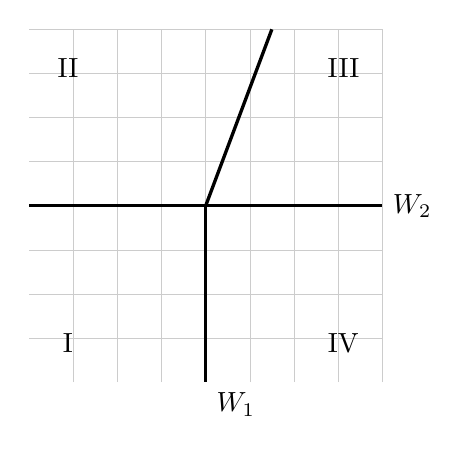
\begin{tikzpicture}[scale=0.7]

  % light square grid
  \draw[step=0.8cm,very thin,color=gray!40] (-3.2,-3.2) grid (3.2,3.2);

  % coordinate axes = walls
  \draw[very thick] (-3.2,0) -- (3.2,0) node[right] {$W_2$};
  \draw[very thick] (0,0) -- (0,-3.2) node[below right] {$W_1$};

  % slanted wall (ray) in quadrant III
  \draw[very thick] (0,0) -- (1.2,3.2);

  % chamber labels
  \node at (-2.5,-2.5) {$\mathrm{I}$};
  \node at (-2.5, 2.5) {$\mathrm{II}$};
  \node at ( 2.5, 2.5) {$\mathrm{III}$};
  \node at ( 2.5,-2.5) {$\mathrm{IV}$};

\end{tikzpicture}
\end{center}

\begin{itemize}
\item Let
\[
\cV = \cO_{\P^2_x\times\P^2_y}(-2,0)\oplus
      \cO_{\P^2_x\times\P^2_y}(-1,-3),
\]
and consider $\mathrm{tot}(\cV)$ as a toric variety given as a GIT
quotient of $\A^8$ by a torus $T\cong(\C^\ast)^2$ with weight matrix
$(t, s) \mapsto (t, t, t, s, s, s, t^{-2}, t^{-1}s^{-3})$.

\item For each wall $W_i$ there is a Kirwan-Ness stratification near
$W_i$ (Table~1 in \cite{HLS}).  The least unstable stratum has fixed
locus $Z_i$ and Levi quotient $L_i$, so that the local GIT quotient for
the wall is $Z_i/L_i$.

\item One introduces a Landau-Ginzburg potential
\[
W = p f + q g \in \C[x_i,y_j,p,q]_{\deg=2},
\]
where $f$ has bidegree $(2,0)$ and $g$ has bidegree $(1,3)$, and $f$ cuts out a smooth rational curve on $\P^2_x$.
  The LG
pair $(\cV,W)$ carries a second $\C^\ast$-grading (the LG grading, "R-charge") so that the variables $p,q$ have weight
$2$ and the $x_i,y_j$ have weight $0$, so that $W$ has weight
$2$; the associated category $D^b(\cV,W)$ is equivalent to $D^b(X)$.

  The key point is that, although $Z_i/L_i$ is \emph{non-compact} as a
  usual GIT quotient, the restriction $W|_{Z_i}$ makes the LG quotient
  $(Z_i/L_i,W|_{Z_i})$ effectively compact.  Concretely:
  \begin{itemize}
  \item Near $W_1$ one has $Z_1/L_1 \cong \P^2/\C^\ast$; the LG
        category $D^b(Z_1/L_1,W|_{Z_1})$ is equivalent to
        $D^b(\P^2)$, which admits the full exceptional collection
        $\langle \cO,\cO(1),\cO(2)\rangle$.
  \item Near $W_2$ one has $Z_2/L_2 \cong \mathrm{tot}\,\cO_{\P^2}(-2)/\C^\ast$;
        the potential restricts to $pf$. Then
        $D^b(Z_2/L_2,W|_{Z_2})\simeq D^b(C)$, and for each window this is
        equivalent to $D^b(\P^1)$ with its exceptional pair
        $\langle\cO,\cO(1)\rangle$.
  \end{itemize}

\item One finds:
  \begin{itemize}
  \item the window shift across $W_1$ is a composition of spherical
        twists around the line bundles
        \[
        \cO_X(0,i),\ \cO_X(0,i+1),\ \cO_X(0,i+2),
        \]
  \item the window shift across $W_2$ is a composition of spherical
        twists around
        \[
        \cO_X(i,0),\ \cO_X(i+1,0),
        \]
  for suitable integers $i$ (depending on the chosen windows).
  \end{itemize}
\end{itemize}

Thus, in this example the abstract window-shift autoequivalences
arising from VGIT of $(\cV,W)$ are identified explicitly with
compositions of spherical twists by line bundles on the K3 surface $X$.
\end{example}

\section{Derived categories}
In this appendix we collect some definitions and facts about derived categories. We prove the classical reconstruction theorem of Bondal-Orlov \cite{BondalOrlov2001} for varieties with ample or anti-ample canonical bundle.
\subsection{Basic definitions}
Let $\mathcal{A}$ be an abelian category. The derived category $D(\mathcal{A})$ is constructed in several steps. Consider the category $C(\mathcal{A})$ of complexes in $\mathcal{A}$, whose objects are cochain complexes and morphisms are chain maps that commute with the differentials.  

Form the homotopy category $K(\mathcal{A})$ whose objects are the same as $C(\mathcal{A})$. The morphisms are chain maps modulo homotopy equivalence. Two chain maps \[f,g:A^\bullet\to B^\bullet\] are homotopic if there exist morphisms $h^i:A^i\to B^{i-1}$ such that \[f^i - g^i = d_B^{i-1} \circ h^i + h^{i+1} \circ d_A^i\] It is a routine check that two maps which are homotopic induce the same map on cohomology.

Finally form $D(\mathcal{A})$ by formally inverting all quasi-isomorphisms in $K(\mathcal{A})$. The morphisms in $D(\mathcal{A})$ are a little subtle. For example, one cannot just introduce formal inverses to quasi-isomorphisms. If $X$ is not an injective object in $\mathcal{A}$, then the inclusion map $X[0] \to I^\bullet$ into an injective resolution is a quasi-isomorphism. If we formally invert by introducing $p: I^\bullet \to X[0]$ with \begin{align*}
    [p] \circ [i] = [\mathrm{id}_{X[0]}] \quad \text{in } K(\mathcal{A}) \\
    [i] \circ [p] = [\mathrm{id}_{I^\bullet}] \quad \text{in } K(\mathcal{A})
  \end{align*} then by definition, we impose that $i,p$ are homotopy equivalences.  This is too strong, since not every quasi-isomorphism is a homotopy equivalence.

Abstractly, let $S$ be the set of quasi-isomorphisms in $K(\mathcal{A})$. The derived category \[D(\mathcal{A}) = K(\mathcal{A})[S^{-1}]\] is characterized by a universal property: there is a functor
  \[
  Q : K(\mathcal{A}) \longrightarrow D(\mathcal{A})
  \]
  sending every $s \in S$ to an isomorphism, and universal with that property (any other functor inverting all quasi-isomorphisms factors uniquely through $Q$). One can also describe morphisms in $D(\mathcal{A})$ concretely as "roofs" via Verdier localization. The bounded derived category $D^b(\mathcal{A})$ is the full subcategory of complexes with bounded cohomology.

  \begin{definition}
    [Mapping cone] For a chain map $s:X^\bullet\to I^\bullet$ (cohomological grading), the \textbf{mapping cone} $\mathrm{Cone}(s)$ is the complex
    \[
    \mathrm{Cone}(s)^n = I^n \oplus X^{n+1}, \qquad d(b,a) = \big(d_I b + s(a),\; -d_X a\big).
    \]
  \end{definition} 
  There's a short exact sequence of complexes
    \[
    0\to I^\bullet \xrightarrow{\iota} \mathrm{Cone}(s) \xrightarrow{\pi} X^\bullet[1]\to 0,
    \]
  giving rise to a long exact sequence in cohomology
    \[\cdots \to H^{n}(I^\bullet) \xrightarrow{H^n(\iota)} H^{n}(\mathrm{Cone}(s)) \xrightarrow{H^n(\pi)} H^{n+1}(X^\bullet) \xrightarrow{H^{n+1}(s)} H^{n+1}(I^\bullet) \to \cdots\]

    \begin{proposition}
      Let $s:X^\bullet\to I^\bullet$ be a chain map in $C(\mathcal{A})$. Then:
      \begin{enumerate}
        \item $s$ is a quasi-isomorphism if and only if $\mathrm{Cone}(s)$ is acyclic (all cohomology groups vanish).

        \item $s$ is an isomorphism in $K(\mathcal{A})$ (i.e., a homotopy equivalence) if and only if $\mathrm{Cone}(s)$ is contractible (chain-homotopic to 0).
      \end{enumerate}
    \end{proposition}

\begin{proof}
  \leavevmode
\begin{enumerate}
  \item ($\Rightarrow$) If $s$ is a quasi-isomorphism, then each $H^{n+1}(s)$ is an isomorphism. In the exact segment 
  \[
  H^n(I)\to H^n(\mathrm{Cone}(s))\to H^{n+1}(X)\xrightarrow{H^{n+1}(s)} H^{n+1}(I),
  \]
  the image of $H^n(\mathrm{Cone}(s))\to H^{n+1}(X)$ is $\ker H^{n+1}(s)=0$, so $H^n(I)\to H^n(\mathrm{Cone}(s))$ is surjective. Looking one step earlier,
  \[
  H^{n}(X)\xrightarrow{H^{n}(s)} H^{n}(I)\to H^n(\mathrm{Cone}(s)),
  \]
  the image of $H^{n}(s)$ is all of $H^{n}(I)$, so the map $H^{n}(I)\to H^n(\mathrm{Cone}(s))$ has zero kernel. Combining "surjective" and "zero kernel" forces $H^n(\mathrm{Cone}(s))=0$ for all $n$. So $\mathrm{Cone}(s)$ is acyclic.

  ($\Leftarrow$) If $\mathrm{Cone}(s)$ is acyclic, then $H^n(\mathrm{Cone}(s))=0$ for all $n$. The exact segment becomes
  \[
  0\to H^{n+1}(X)\xrightarrow{H^{n+1}(s)} H^{n+1}(I)\to 0,
  \]
  so each $H^{n+1}(s)$ is an isomorphism. Hence $s$ is a quasi-isomorphism.


  \item If $s$ has a homotopy inverse $t$ (so $ts\simeq \mathrm{id}_X$, $st\simeq \mathrm{id}_I$), then the triangle
  \[
  X^\bullet \xrightarrow{s} I^\bullet \to \mathrm{Cone}(s) \to X^\bullet[1]
  \]
  is isomorphic (in $K$) to
  \[
  X^\bullet \xrightarrow{\mathrm{id}} X^\bullet \to \mathrm{Cone}(\mathrm{id}_X) \to X^\bullet[1].
  \]

  For any complex $X^\bullet$, $\mathrm{Cone}(\mathrm{id}_X)$ is contractible with contracting homotopy
  \[
  H^n : X^n \oplus X^{n+1} \longrightarrow X^{n-1} \oplus X^{n},\qquad
  H^n(x,y)=(0,x).
  \]
  One can check that $dH+Hd=\mathrm{id}$. Thus $\mathrm{Cone}(s)$ is contractible. \qedhere
  \end{enumerate}
\end{proof}
\begin{example}
  Let $\mathcal{A}=\mathbf{Ab}$. Take the injective resolution of $\mathbb{Z}$:
  \[
  0 \to \mathbb{Z} \xrightarrow{i} \mathbb{Q} \xrightarrow{q} \mathbb{Q}/\mathbb{Z} \to 0
  \]
  and regard $I^\bullet$ as $I^0=\mathbb{Q}$, $I^1=\mathbb{Q}/\mathbb{Z}$ with $d^0=q$, and $X^\bullet=\mathbb{Z}[0]$. The resolution map $s:\mathbb{Z}[0]\to I^\bullet$ has $s^0=i$.

  Compute the cone. By the definition above,
  \[
  \mathrm{Cone}(s)^{-1}=\mathbb{Z},\quad
  \mathrm{Cone}(s)^0=\mathbb{Q},\quad 
  \mathrm{Cone}(s)^1=\mathbb{Q}/\mathbb{Z}
  \]
  with differentials $d^{-1}=i:\mathbb{Z}\to\mathbb{Q}$ and $d^{0}=q:\mathbb{Q}\to\mathbb{Q}/\mathbb{Z}$. So $\mathrm{Cone}(s)$ is exactly the three-term complex sitting in degrees $-1,0,1$.
  \[
  \mathbb{Z} \xrightarrow{i} \mathbb{Q} \xrightarrow{q} \mathbb{Q}/\mathbb{Z}
  \]
  The cone is acyclic: the short exact sequence $0\to \mathbb{Z} \to \mathbb{Q} \to \mathbb{Q}/\mathbb{Z} \to 0$ is exact, so the cone's cohomology vanishes. However, it is not contractible: contractibility of this 3-term exact complex is equivalent to the short exact sequence splitting (a contracting homotopy gives splittings and vice versa). But $0\to \mathbb{Z} \to \mathbb{Q} \to \mathbb{Q}/\mathbb{Z} \to 0$ does not split: if it did, $\mathbb{Z}$ would be a direct summand of the divisible group $\mathbb{Q}$, hence divisible itself, which is false.

  Therefore $s$ is a quasi-isomorphism whose cone is acyclic but not contractible; hence $s$ is not a homotopy equivalence and cannot be inverted in $K(\mathcal{A})$.
\end{example}

\begin{definition}
  [Triangulated category] A \textbf{triangulated category} is an additive category $\mathcal{T}$ equipped with an autoequivalence $[1]:\mathcal{T}\to\mathcal{T}$ (the shift functor) and a class of distinguished triangles
  \[X \xrightarrow{f} Y \xrightarrow{g} Z \xrightarrow{h} X[1]\]
  satisfying the following axioms:
  \begin{itemize}
    \item (TR1) For every morphism $f:X\to Y$ in
          $\mathcal{T}$, there exists a distinguished triangle
          \[
            X \xrightarrow{f} Y \longrightarrow Z \longrightarrow X[1].
          \]
          Moreover, for every object $X\in\mathcal{T}$, the triangle
          \[
            X \xrightarrow{\mathrm{id}_X} X \longrightarrow 0 \longrightarrow X[1]
          \]
          is distinguished, and any triangle isomorphic to a distinguished triangle is distinguished.
    \item (TR2) A triangle
          \[X \xrightarrow{f} Y \xrightarrow{g} Z \xrightarrow{h} X[1]\]
          is distinguished if and only if the rotated triangle
          \[Y \xrightarrow{g} Z \xrightarrow{h} X[1] \xrightarrow{-f[1]} Y[1]\]
          is distinguished.
    \item (TR3) Given two distinguished triangles
          \[X \xrightarrow{f} Y \xrightarrow{g} Z \xrightarrow{h} X[1]\]
                and
                \[U \xrightarrow{p} V \xrightarrow{q} W \xrightarrow{r} U[1],\]
                and morphisms $a:X\to U$, $b:Y\to V$ such that $b\circ f = p \circ a$, there exists a morphism $c:Z\to W$ making the following diagram commute:
                \[
\begin{tikzcd}
X \arrow[r,"f"] \arrow[d,"a"'] 
  & Y \arrow[r,"g"] \arrow[d,"b"'] 
  & Z \arrow[r,"h"] \arrow[d,"c"'] 
  & X[1] \arrow[d,"{a[1]}"] \\
U \arrow[r,"p"'] 
  & V \arrow[r,"q"'] 
  & W \arrow[r,"r"'] 
  & U[1]
\end{tikzcd}
\]
          
    \item (TR4) (Octahedral axiom) Given morphisms $X \xrightarrow{f} Y \xrightarrow{g} Z$ in $\mathcal{T}$, there exist distinguished triangles
          \[X \xrightarrow{f} Y \xrightarrow{u} C(f) \xrightarrow{v} X[1],\]
          \[Y \xrightarrow{g} Z \xrightarrow{u'} C(g) \xrightarrow{v'} Y[1],\]
          and
          \[X \xrightarrow{g\circ f} Z \xrightarrow{u"} C(g\circ f) \xrightarrow{v"} X[1],\]
          along with morphisms $C(f) \xrightarrow{w} C(g\circ f)$ and $C(g) \xrightarrow{w'} C(g\circ f)$ such that the following diagram commutes and the rows and columns are distinguished triangles:
          \[\begin{tikzcd}
            & Y \arrow[rr, "u"] \arrow[dd, "g"'] & & C(f) \arrow[dd, "w"] \\
            X \arrow[ur, "f"] \arrow[dr, "g\circ f"'] & & & \\
            & Z \arrow[rr, "u'"'] & & C(g)
          \end{tikzcd}\]
  \end{itemize}
\end{definition}

\begin{proposition}
  This construction gives $D(\mathcal{A})$ the structure of a triangulated category, where:
\begin{itemize}
  \item The shift functor $[1]$ moves complexes one place to the left:
  \[X^\bullet[1]^n = X^{n+1}, \quad d_{X[1]}^n = -d_X^{n+1}\]
  \item Distinguished triangles come from mapping cones of chain maps, in particular, for any chain map $f:X^\bullet\to Y^\bullet$, the triangle
  \[X^\bullet \xrightarrow{f} Y^\bullet \to \mathrm{Cone}(f) \to X^\bullet[1]\]
  is distinguished
  \item The cohomology functors are first defined on the homotopy category as functors \[H^i_K: K(\mathcal{A}) \to \mathcal{A}\] Since these functors send quasi-isomorphisms to isomorphisms, they descend through the localization map $Q: K(\mathcal{A}) \to D(\mathcal{A})$. In particular, there exists a unique functor \[H^i_D: D(\mathcal{A}) \to \mathcal{A}\] such that $H^i_K = H^i_D \circ Q$.
\end{itemize}
\end{proposition}

In the Bondal-Orlov paper, they work with more relaxed categories known as graded categories. In particular every triangulated category is a graded category.
\begin{definition}[Graded categories and exact functors]
A \textbf{graded category} is a pair $(\mathcal{D}, T_{\mathcal{D}})$ consisting of a category $\mathcal{D}$ and a fixed autoequivalence
\[
T_{\mathcal{D}} : \mathcal{D} \longrightarrow \mathcal{D},
\]
called the \textbf{translation functor}.


A functor
\[
F : \mathcal{D} \longrightarrow \mathcal{D}'
\]
between graded categories is called \textbf{graded} if it commutes with the translation functors.
More precisely, there is a fixed natural isomorphism of functors
\[
t_F : F \circ T_{\mathcal{D}} \;\xrightarrow{\sim}\; T_{\mathcal{D}'} \circ F.
\]
A natural transformation $\mu : F \Rightarrow G$ between graded functors is called \textbf{graded}
if the following diagram commutes:
\[
\begin{tikzcd}
F \circ T \arrow[r, "t_F"] \arrow[d, "\mu T"'] & T \circ F \arrow[d, "T\mu"] \\
G \circ T \arrow[r, "t_G"'] & T \circ G.
\end{tikzcd}
\]


A graded functor
\[
F : \mathcal{D} \longrightarrow \mathcal{D}'
\]
between triangulated categories is called \textbf{exact} if it sends exact triangles
to exact triangles in the following sense.

If
\[
X \xrightarrow{f} Y \xrightarrow{g} Z \xrightarrow{h} T X
\]
is an exact triangle in $\mathcal{D}$, then one replaces the segment
\[
F T(X)
\]
by
\[
T F(X)
\]
via the natural isomorphism $t_F : F T \xrightarrow{\sim} T F$,
and requires that the resulting sequence
\[
F X \xrightarrow{F f} F Y \xrightarrow{F g} F Z \xrightarrow{t_F(Fh)} T F X
\]
be an exact triangle in $\mathcal{D}'$.

Finally, a \textbf{morphism between exact functors} is, by definition,
a graded natural transformation.
\end{definition}

\begin{proposition}
Let $F : \mathcal{D} \longrightarrow \mathcal{D}'$ be a graded functor between graded categories, and let
$G : \mathcal{D}' \longrightarrow \mathcal{D}$
be its left adjoint, so that the unit and counit of the adjunction are the natural transformations
\[
\operatorname{id}_{\mathcal{D}'} \xrightarrow{\ \alpha\ } F \circ G, 
\qquad
G \circ F \xrightarrow{\ \beta\ } \operatorname{id}_{\mathcal{D}}.
\]
Then \(G\) can be canonically endowed with the structure of a graded functor, so that the unit and counit of the adjunction become morphisms of graded functors. If, in addition, \(F\) is an exact functor between triangulated categories, then \(G\) also becomes an exact functor.
\end{proposition}


\begin{definition}
  
Let $\mathcal{D}$ be a $k$-linear category with finite-dimensional $\mathrm{Hom}$'s.
A covariant additive functor
\[
S : \mathcal{D} \longrightarrow \mathcal{D}
\]
is called a \textbf{Serre functor} if it is a category equivalence and there are given bifunctorial isomorphisms
\[
\varphi_{A,B} : \mathrm{Hom}_{\mathcal{D}}(A,B) \;\xrightarrow{\ \sim\;}\; \mathrm{Hom}_{\mathcal{D}}(B,SA)^{*}
\]
for all $A,B \in \mathcal{D}$, such that the following diagram is commutative:
\[
\begin{tikzcd}
\mathrm{Hom}_{\mathcal{D}}(A,B)
  \arrow[r,"\varphi^{A,B}"]
  \arrow[d]
  & \mathrm{Hom}_{\mathcal{D}}(B,SA)^{*}
  \arrow[d] \\
\mathrm{Hom}_{\mathcal{D}}(SA,SB)
  \arrow[r,"\varphi^{SA,SB}"']
  & \mathrm{Hom}_{\mathcal{D}}(SB,S^{2}A)^{*}
\end{tikzcd}
\]
The vertical isomorphisms in this diagram are those induced by $S$.

\end{definition}

\begin{proposition}
Any autoequivalence
\[
\Phi : \mathcal{D} \longrightarrow \mathcal{D}
\]
commutes with a Serre functor, i.e.\ there exists a natural graded isomorphism of functors
\[
\Phi \circ S \;\xrightarrow{\;\sim\;}\; S \circ \Phi.
\]
\end{proposition}

\begin{proof}
For any pair of objects $A,B \in \mathcal{D}$, we have a system of natural isomorphisms:
\[
\mathrm{Hom}(\Phi A, \Phi SB)
  \;\cong\;
\mathrm{Hom}(A, SB)
  \;\cong\;
\mathrm{Hom}(B, A)^{*}
  \;\cong\;
\mathrm{Hom}(\Phi B, \Phi A)^{*}
  \;\cong\;
\mathrm{Hom}(\Phi A, S\Phi B).
\]
Since $\Phi$ is an equivalence, the essential image of $\Phi$ covers all of $\mathcal{D}$; that is,
every object is isomorphic to some $\Phi A$.
Hence we have isomorphisms of contravariant functors represented by the objects
$\Phi SB$ and $S\Phi B$.
By Brown's representability lemma, morphisms between representable functors correspond
bijectively to morphisms between their representing objects.
This yields a canonical isomorphism
\[
\Phi SB \;\xrightarrow{\;\sim\;}\; S\Phi B,
\]
which is in fact natural in $B$.
\end{proof}
A Serre functor in a category $\mathcal{D}$, if it exists, is unique up to a graded natural isomorphism. By definition it is intrinsically related to the structure of the category.
We shall use this later to reconstruct a variety from its derived category and to find
the group of exact autoequivalences for algebraic varieties with ample either canonical
or anticanonical sheaf.

\subsection{Reconstruction theorem}
Let $X$ be a smooth projective variety over a field $k$ with either ample or antiample canonical sheaf $\omega_X$. Let $n = \dim X$, $\cD = D^b_{\mathrm{coh}}(X)$ be the bounded derived category of coherent sheaves on $X$.

\begin{proposition}
  $\cD$ has a Serre functor $S$ given by
  \[S(-) = - \otimes \omega_X [n]\]
\end{proposition}

\begin{proof}
  Grothendieck-Serre duality gives bifunctorial isomorphisms
  \[\Ext^i_X(F,G) \cong \Ext^{n-i}_X(G, F \otimes \omega_X)^*\]
  for all coherent sheaves $F,G$ on $X$. This extends to complexes in $\cD$ by taking injective resolutions. Thus $S$ is a Serre functor.
\end{proof}
  \begin{definition}[Point object]
An object $P \in \mathcal{D}$ is called a \textbf{point object of codimension $n(P)$} if
\begin{enumerate}
    \item $S_{\mathcal{D}}(P) \simeq P[n(P)]$,
    \item $\Hom^{<0}(P,P) = 0$,
    \item $\Hom^0(P,P) = k(P)$,
\end{enumerate}
where $k(P)$ is a field (automatically a finite extension of the base field $k$).
\end{definition}

\begin{proposition}
Let $X$ be a smooth algebraic variety of dimension $n$ with ample canonical or anticanonical sheaf.  
Then an object $P \in D^b_{\mathrm{coh}}(X)$ is a point object if and only if
\[
P \cong \mathcal{O}_x[r], \qquad r \in \mathbb{Z},
\]
where $\mathcal{O}_x$ is the skyscraper sheaf of a closed point $x \in X$ (up to translation).
\end{proposition}

\begin{proof}
  Since $X$ has an ample invertible sheaf, it is projective. Any skyscraper sheaf of a closed point obviously satisfies the conditions of a point object
with codimension equal to the dimension of the variety.

Suppose now that for some $P \in D^b_{\mathrm{coh}}(X)$ we have that $P$ is a point object of codimension $s$. 
Let $\mathcal{H}^i$ be the cohomology sheaves of $P$.


From (i) we obtain $s = n$. From the Serre functor formula, we have
\[P \otimes \omega_X [n] \;\simeq\; P[s]\]
Because tensoring with an invertible sheaf is an exact functor on the abelian category of coherent sheaves, we can take cohomlogy sheaves
\[\cH^i(P\otimes\omega_X) \cong \cH^i(P)\otimes\omega_X \cong \cH^{i+t}(P)\]
If $t = s - n \neq 0$, then for any $i$ we can iterate this isomorphism to get that infinitely many $\cH^j(P)$ are nonzero, contradicting the boundedness of $P$. Thus $t=0$.


We also get that $\mathcal{H}^i \otimes \omega_X \cong \mathcal{H}^i$.
Since $\omega_X$ is either ample or antiample, it follows that
each $\mathcal{H}^i$ is a finite-length sheaf, i.e.\ its support consists of isolated points. 

\begin{remark}
  In general, if $\mathcal{F}$ is a coherent sheaf on a projective variety $X$ such that $\mathcal{F} \otimes \mathcal{L} \cong \mathcal{F}$ for an ample line bundle $\mathcal{L}$, then $\mathcal{F}$ is supported at finitely many points. Examining the Hilbert polynomial of $\mathcal{H}^i \otimes \omega_X^{\otimes m}$ for $m \gg 0$ shows that the dimension of the support of $\mathcal{F}$ must be zero.
\end{remark}


Sheaves supported at different points are homologically orthogonal, so $P$ decomposes into a direct sum of components supported at single points. This is because Ext groups are computed locally, i.e. for every open $U\subset X$,
\[
\mathcal{E}xt^p_X(\mathcal{F},\mathcal{G})|_U
\;\cong\;
\mathcal{E}xt^p_U(\mathcal{F}|_U,\mathcal{G}|_U),
\]
and the support of $\mathcal{E}xt^p_X(\mathcal{F},\mathcal{G})$ is contained in $\operatorname{Supp}(\mathcal{F}) \cap \operatorname{Supp}(\mathcal{G})$.



By (iii), $P$ is indecomposable. In particular, if $P = P_1 \oplus P_2$ with $P_1,P_2$ supported at different points, then $\End(P)$ would contain nontrivial idempotents, contradicting (iii). 

There is a standard spectral sequence (coming from the stupid filtration on $P$ and the $t$-structure) computing self-Exts of $P$ from Exts between its cohomology sheaves:
\[
E_2^{p,q}
= \bigoplus_{i\in\Z}
\Ext^p\bigl(\cH^i,\ \cH^{i+q}\bigr)
\;\Longrightarrow\;
\Hom^{p+q}(P,P).
\]
\begin{remark}
The spectral sequence used above arises instead from the general fact that any filtered complex carries a canonical spectral sequence. General spectral sequence theory for filtered complexes says if $(K^\bullet, F^\bullet)$ is a filtered complex in an abelian category (or more generally in a suitable derived context), there is a spectral sequence
\[
E_1^{p,q} = H^{p+q}\bigl(\operatorname{Gr}^p_F K^\bullet\bigr)
\;\Longrightarrow\;
H^{p+q}(K^\bullet)
\]
Here the associated graded pieces are the complexes $\operatorname{Gr}^p_F K^\bullet = F^p K^\bullet / F^{p-1}K^\bullet$ obtained by taking successive quotients of the filtration. The differentials in the spectral sequence come from the differentials in the original complex $K^\bullet$ and from the filtration structure.  

Let $D^b(\Coh X)$ carry its standard $t$--structure, with truncations
$\tau_{\le i},\tau_{\ge i}$ and cohomology sheaves $\cH^i(-)$.

Fix $P\in D^b(\Coh X)$, and consider the stupid filtration of $P$:
\[
\cdots \subset P_{\le i-1} \subset P_{\le i} \subset P_{\le i+1} \subset \cdots
\]
where
\[
P_{\le i} = 
\cdots \to P^{n-2} \to P^{n-1} \to P^{n} \to 0 \to 0 \to \cdots
\]
and each successive quotient fits into a triangle
\[
\cH^i(P)[-i] \longrightarrow P_{\le i} \longrightarrow P_{\le i-1} \longrightarrow \cH^i(P)[-i+1].
\]
Thus the \emph{associated graded} of this filtration is
\[
\Gr^i P \;\simeq\; \cH^i(P)[-i].
\]

Now apply the derived functor
\[
\mathbf R\Hom(-,P): D^b(\Coh X)^{op}\longrightarrow D^b(\mathrm{Vect}_k)
\]
to this filtered object.  We obtain a decreasing filtration
\[
\cdots \subset F^{i+1}C \subset F^i C \subset F^{i-1}C \subset \cdots
\]
on the complex
\[
C := \mathbf R\Hom(P,P)
\]
defined by
\[
F^i C := \mathbf R\Hom(P_{\le i},P).
\]
The successive quotients of this filtration are
\[
\Gr^i C
:= F^iC/F^{i+1}C
\simeq \mathbf R\Hom(\Gr^i P,P)
\simeq \mathbf R\Hom(\cH^i(P)[-i],P)
\simeq \mathbf R\Hom(\cH^i(P),P)[-i].
\]
In our situation,
\[
E_1^{p,q}
  = H^{p+q}\bigl(\Gr^p C\bigr)
  \cong
  H^{p+q}\bigl(\mathbf R\Hom(\cH^p(P),P)[-p]\bigr)
  \cong
  H^{p+q-p}\bigl(\mathbf R\Hom(\cH^p(P),P)\bigr).
\]
But
\[
H^{r}\bigl(\mathbf R\Hom(\cH^p(P),P)\bigr)
  \;\cong\;
  \Ext^r\bigl(\cH^p(P),P\bigr),
\]
so we get
\[
E_1^{p,q}
  \;\cong\;
  \Ext^{q}\bigl(\cH^p(P),P\bigr).
\]
To compute the $E_2$ page, we take cohomology with respect
to the first differential \(d_1 : E_1^{p,q} \to E_1^{p+1,q}\), i.e.
cohomology along the \(p\)-direction.

Let \(A\in\mathcal A\) and \(B^\bullet\in D^b(\mathcal A)\) be bounded.
Filter \(B^\bullet\) by its stupid truncations
\[
B_{\le i}^\bullet,\qquad
\Gr^i B^\bullet \simeq \cH^i(B^\bullet)[-i].
\]
Apply \(\mathbf R\Hom(A,-)\). This gives a decreasing filtration
\[
G^i K
:= \mathbf R\Hom\bigl(A,B_{\le i}^\bullet\bigr)\subset
   \mathbf R\Hom\bigl(A,B^\bullet\bigr)=:K
\]
of the complex \(K = \mathbf R\Hom(A,B^\bullet)\).
The associated graded pieces are
\[
\Gr^i K
:= G^iK/G^{i-1}K
\simeq \mathbf R\Hom\bigl(A,\Gr^i B^\bullet\bigr)
\simeq \mathbf R\Hom\bigl(A,\cH^i(B^\bullet)[-i]\bigr)
\simeq \mathbf R\Hom\bigl(A,\cH^i(B^\bullet)\bigr)[-i].
\]

The spectral sequence of this filtered complex has
\[
{}^{(A,B)}E_1^{i,j}
  = H^{i+j}(\Gr^i K)
  \cong
  H^{j}\mathbf R\Hom\bigl(A,\cH^i(B^\bullet)\bigr)
  \cong
  \Ext^{j}\bigl(A,\cH^i(B^\bullet)\bigr),
\]
and converges to
\[
H^{i+j}(K) \cong \Ext^{i+j}(A,B^\bullet).
\]

Reindexing by writing \(j = q\) and \(i = r\), the \(E_2\)-page of this
spectral sequence is (by definition: cohomology of \({}^{(A,B)}E_1\) with
respect to its first differential)
\[
{}^{(A,B)}E_2^{r,s}
  \;\cong\;
  \Ext^{r}\bigl(A,\cH^{s}(B^\bullet)\bigr),
\]
and it converges to
\(\Ext^{r+s}(A,B^\bullet)\).

Now fix \(p\). For the column
\[
E_1^{p,\bullet}
  = \Ext^\bullet\bigl(\cH^p(P^\bullet),P^\bullet\bigr)
\]
take \(A = \cH^p(P^\bullet)\), \(B^\bullet = P^\bullet\) in the above
construction. We get a spectral sequence
\[
{}^{(p)}E_2^{r,s}
  \;\cong\;
  \Ext^r\bigl(\cH^p(P^\bullet),\cH^{s}(P^\bullet)\bigr)
  \;\Longrightarrow\;
  \Ext^{r+s}\bigl(\cH^p(P^\bullet),P^\bullet\bigr)
  = E_1^{p,r+s}.
\]

Thus, for each fixed \(p\), the graded group
\(E_1^{p,\bullet} = \Ext^\bullet(\cH^p(P),P)\) is itself computed by a
second spectral sequence whose \(E_2\)-page consists of the groups
\(\Ext^r(\cH^p(P),\cH^s(P))\).

The spectral sequence attached to the filtration \(F^\bullet C\) is
built from the bigraded object
\[
E_1^{p,q} = \Ext^q\bigl(\cH^p(P^\bullet),P^\bullet\bigr)
\]
together with the differentials \(d_1 : E_1^{p,q}\to E_1^{p+1,q}\).
By general spectral sequence formalism, the \(E_2\)-page is obtained by
taking cohomology of this \(E_1\) with respect to \(d_1\). Equivalently,
it is the page you get after “resolving” each \(E_1^{p,q}\) via the
hyper--\(\Ext\) spectral sequence of Step~1 and keeping track of the
total degree.

Concretely, the total degree of the original spectral sequence is
\(p+q\). The contribution in bidegree \((p,q)\) on the \(E_2\)-page
comes from all classes of total degree \(p+q\) in the various
\(\Ext^\bullet(\cH^i(P),P)\) that survive to the \(E_2\)-page of their
internal hyper--\(\Ext\) spectral sequences. For each cohomological
index \(i\), these internal \(E_2\)-terms are
\[
{}^{(i)}E_2^{p,\,i+q}
  \;\cong\;
  \Ext^p\bigl(\cH^i(P^\bullet),\cH^{i+q}(P^\bullet)\bigr),
\]
and they land in total degree
\[
p + (i+q) - i = p+q.
\]
Summing over all \(i\in\mathbb Z\) gives precisely
\[
E_2^{p,q}
  \;\cong\;
  \bigoplus_{i\in\mathbb Z}
  \Ext^p_{\mathcal A}\bigl(\cH^i(P^\bullet),\cH^{i+q}(P^\bullet)\bigr),
\]
which is the claimed description of the \(E_2\)-page.

Since \(P^\bullet\) is bounded, only finitely many \(i\) contribute for
each \((p,q)\); the filtrations involved are finite, and hence both the
inner hyper--\(\Ext\) spectral sequences and the outer one for
\(C = \mathbf R\Hom(P,P)\) are bounded and converge. Thus we have proved the following:

\begin{proposition}\label{prop:hyper-ext-spectral-sequence}
Let \(\mathcal A\) be an abelian category, and let
\(P^\bullet \in D^b(\mathcal A)\) be a bounded complex.
There is a convergent spectral sequence with $E_1$--page
\[E_1^{p,q}
  \;\cong\;
  \Ext^q_{\mathcal A}\bigl(\cH^p(P^\bullet),P^\bullet\bigr)
\]
and $E_2$--page
\[E_2^{p,q}
  \;\cong\;
  \bigoplus_{i\in\mathbb Z}
  \Ext^p_{\mathcal A}\bigl(\cH^i(P^\bullet),\cH^{i+q}(P^\bullet)\bigr)
\]
converging to
\(\Hom^{p+q}(P^\bullet,P^\bullet)\).
\end{proposition}
\end{remark}

If two cohomology sheaves are nonzero, a negative-degree class appears.
Assume for contradiction that $\cH^i$ and $\cH^j$ are both nonzero for
some $i<j$.  Since all $\cH^k$ are supported at the same closed point,
the sheaves $\cH^i$ and $\cH^j$ are finite--length $\cO_{X,x}$--modules.
For such modules it is standard that
\[
\Hom(\cH^j,\cH^i)\neq 0,
\]
because any nonzero finite--length module possesses a simple quotient,
and any nonzero finite--length module contains a copy of that simple
module.

Such a map $\phi:\cH^j\to\cH^i$ determines a nonzero class
\[
0\neq [\phi] \in E_2^{0,\;i-j},
\]
where $i-j<0$.  
Among all nonzero classes in $E_2^{0,q}$ with $q<0$, choose one with
$q_0$ \emph{minimal} (i.e.\ the most negative possible).

This class cannot be killed by any differential.
The possible outgoing differentials from $E_r^{0,q_0}$ have targets
\[
E_r^{r,\;q_0-r+1},\qquad r\ge 2.
\]
But $q_0-r+1 < q_0$, and by minimality of $q_0$ there are \emph{no}
nonzero entries with $q<q_0$ at the $E_2$--page, hence none at any
later page.  Therefore all outgoing differentials vanish.

The possible incoming differentials come from
\[
E_r^{-r,\;q_0+r-1},
\]
but $p=-r<0$ forces $\Ext^p(-,-)=0$, so these groups are always zero.
Thus there are no incoming differentials either. Hence the class $[\phi]$ survives to the limit:
\[
0\neq[\phi]\in E_\infty^{0,\;q_0}.
\]

Since the spectral sequence abuts to
$\Hom^{m}(P,P)$ with $m=p+q$, our surviving class contributes
\[
0\neq[\phi]\in \Hom^{\,q_0}(P,P).
\]
But $q_0<0$, contradicting the assumption that
$\Hom^m(P,P)=0$ for all negative $m$.

Thus it is impossible for two distinct cohomology sheaves $\cH^i$ and
$\cH^j$ to be nonzero.  Therefore $P$ has a single nonzero
cohomology sheaf:
\[
P \simeq \cH^r(P)[-\,r].
\]
Since $\End(P)=\End(\cH^r)$ is a field, the sheaf $\cH^r$ must be an
indecomposable finite--length $\cO_{X,x}$--module whose endomorphism
ring has no nontrivial idempotents.  The only such modules are the
simple ones.  Thus $\cH^r \cong k(x)$ is a skyscraper sheaf at a closed
point.
\end{proof}

\begin{definition}[Invertible object]\label{def:invertible-object}
An object \(L\in \mathcal D\) is called \emph{invertible} if for any point
object \(P\in\mathcal D\) there exists an \(s\in\mathbb Z\) such that
\begin{enumerate}
  \item[(i)] \(\Hom^{s}(L,P)=k(P)\),
  \item[(ii)] \(\Hom^{i}(L,P)=0\) for \(i\ne s\).
\end{enumerate}
\end{definition}

\begin{proposition}\label{prop:invertible-objects-are-shifts}
Let \(X\) be a smooth irreducible algebraic variety.  Assume that all
point objects have the form \(\mathcal O_{x}[s]\) for some \(x\in X\),
\(s\in\mathbb Z\).  Then an object \(L\in\mathcal D\) is invertible if
and only if \(L\simeq \mathcal L[t]\) for some invertible sheaf
\(\mathcal L\) on \(X\) and some \(t\in\mathbb Z\).
\end{proposition}

\begin{proof}
For an invertible sheaf \(\mathcal L\) we have
\[
  \Hom(\mathcal L,\mathcal O_{x}) = k(x),\qquad
  \Ext^{i}(\mathcal L,\mathcal O_{x}) = 0,\quad \text{if } i\ne 0.
\]
Therefore, if \(L=\mathcal L[s]\), then it is an invertible object.

Suppose $L$ is an invertible object in $D^b(X)$ and let $m$ be maximal
 such that $\mathcal H^m := \mathcal H^m(L)\neq 0$.   

From the truncation triangle
\[\tau_{\le m-1}L \longrightarrow L \longrightarrow \mathcal H^{m}[-m]\]
and the assumption that $m$ is maximal with $\mathcal H^{m}(L)\neq 0$, one knows that $\tau_{\le m-1}L$ has cohomology only in degrees $< m$. Thus applying \(\Hom(-,\mathcal O_{x_0})\) shows that \(\Hom(\tau_{\le m-1}L, k(x_0)[t])=0\) for $t\ge -m$ and in particular the map $L \longrightarrow \mathcal H^{m}[-m]$ induces isomorphisms on all \(\Hom(-,k(x_0)[t])\) for $t\ge -m$.



Pick a point $x_0\in \operatorname{supp}(\mathcal H^m)$.  
Then there exists a nontrivial homomorphism
\[
   \mathcal H^m \longrightarrow k(x_0).
\]
This is because the stalk
$M := \mathcal H^m_{x_0}$ is a nonzero finitely generated
$\mathcal O_{X,x_0}$–module. Let $R := \mathcal O_{X,x_0}$, with maximal
ideal $\mathfrak m_{x_0}$ and residue field $k(x_0)=R/\mathfrak m_{x_0}$.
By Nakayama, $M/\mathfrak m_{x_0}M\neq 0$, so $M/\mathfrak m_{x_0}M$ is a
nonzero finite–dimensional $k(x_0)$–vector space. Choose a nonzero
$k(x_0)$–linear functional
\[
\ell : M/\mathfrak m_{x_0}M \to k(x_0),
\]
and compose with the natural surjection $M\twoheadrightarrow
M/\mathfrak m_{x_0}M$ to obtain a nonzero $R$–linear map
$M\to k(x_0)$. Using the identification
\[
\Hom_X(\mathcal H^m,k(x_0))\cong \Hom_R(M,k(x_0)),
\]
this gives a nontrivial homomorphism of sheaves
$\mathcal H^m\to k(x_0)$.

Hence
\[
  0 \neq \Hom\bigl(\mathcal H^m, k(x_0)\bigr)
    = \Hom\bigl(L, k(x_0)[-m]\bigr),
\]
and the nonvanishing of this group forces the codimension of this point object $n_{k(x_0)} = -m$. Apply the same spectral sequence (Proposition~\ref{prop:hyper-ext-spectral-sequence})
to deduce
\[
E_{2}^{1,-m}
 = \Hom(\mathcal H^{m}, k(x_{0})[1])
 = \Hom\bigl(L, k(x_{0})[1+n_{k(x_{0})}]\bigr)
 = 0.
\]
Thus, as soon as $x_{0}\in X$ is in the support of $\mathcal H^{m}$, we obtain
\[
\Ext^{1}(\mathcal H^{m}, k(x_{0})) = 0.
\]
Next, we shall apply the following standard result in commutative algebra:
Any finite module $M$ over an arbitrary noetherian local ring $(A,\mathfrak m)$
with $\Ext^{1}_{A}(M, A/\mathfrak m)=0$ is free.

The local-to-global spectral sequence
\[
E_{2}^{p,q} = H^{p}\left(X, \cE xt^{q}(\mathcal H^{m}, k(x_{0}))\right)
  \;\Longrightarrow\;
  \Ext^{p+q}(\mathcal H^{m}, k(x_{0}))
\]
allows us to pass from the global vanishing $\Ext^{1}(\mathcal H^{m}, k(x_{0}))=0$
to the local one $\cE xt^{1}(\mathcal H^{m}, k(x_{0}))=0$.  
More precisely, as $\cE xt^{0}(\mathcal H^{m}, k(x_{0}))$ is concentrated at
$x_{0}\in X$, one has
\[
E_{2}^{2,0}
 = H^{2}\left(X, \cE xt^{0}(\mathcal H^{m}, k(x_{0}))\right)
 = 0.
\] since sheaves with zero-dimensional support have vanishing higher cohomology.
  Hence, there are no nontrivial differentials and so
\[
E_{2}^{0,1} = E_{\infty}^{0,1}
\]
Moreover, since $\cE xt^{1}(\mathcal H^{m}, k(x_{0}))$ is also concentrated at $x_{0}\in X$,
it is a globally generated sheaf because it is precisely the data of its stalk at $x_{0}$.
Hence,
\[
H^{0}\left(X, \cE xt^{1}(\mathcal H^{m}, k(x_{0}))\right)
  = E_{2}^{0,1}
  = 0
\]
implies $\cE xt^{1}(\mathcal H^{m}, k(x_{0})) = 0$. But then the aforementioned
result from commutative algebra shows that $\mathcal H^{m}$ is free in a
neighbourhood of $x_{0}\in X$.

Since $X$ is irreducible, we have in particular
$\operatorname{supp}(\mathcal H^{m}) = X$.  
Thereby, there exists for any $x\in X$ a surjection
$\mathcal H^{m} \twoheadrightarrow k(x)$. Hence,
\[
\Hom(L, k(x)[-m]) = \Hom(\mathcal H^{m}, k(x)) \neq 0.
\]
In particular, $n_{k(x)}$ does not depend on $x$. As by assumption,
\[
k(x)
 = \Hom\bigl(L, k(x)[-m]\bigr)
 = \Hom(\mathcal H^{m}, k(x)),
\]
the sheaf $\mathcal H^{m}$ has constant fibre dimension one. Hence
$\mathcal H^{m}$ is a line bundle.
\end{proof}


We are now ready to state and prove the reconstruction theorem.
\begin{theorem}[Reconstruction theorem \cite{BondalOrlov2001}]
Let $X$ and $Y$ be smooth projective varieties over a field $k$
with either ample or antiample canonical sheaf. If there is an exact equivalence of triangulated categories
\[D^b_{\mathrm{coh}}(X) \xrightarrow{\sim} D^b_{\mathrm{coh}}(Y),\]
then $X$ is isomorphic to $Y$.
\end{theorem}

\begin{proof}
Assume that under an equivalence 
\[
F : D^{b}(X) \;\xrightarrow{\;\sim\;}\; D^{b}(Y)
\]
the structure sheaf $\mathcal O_{X}$ is mapped to $\mathcal O_{Y}$.
Since any equivalence is compatible with Serre functors 
and $\dim(X)=\dim(Y)=:n$, this proves
\[
F(\omega_{X}^{k})
 = F\bigl(S_{X}^{k}(\mathcal O_{X})[-kn]\bigr)
 \;\simeq\;
 S_{Y}^{k}\bigl(F(\mathcal O_{X})\bigr)[-kn]
 \;\simeq\;
 S_{Y}^{k}(\mathcal O_{Y})[-kn]
 = \omega_{Y}^{k}.
\]
Using that $F$ is fully faithful, we conclude from this that
\[
H^{0}(X,\omega_{X}^{k})
 = \Hom(\mathcal O_{X},\omega_{X}^{k})
 \simeq \Hom(F(\mathcal O_{X}),F(\omega_{X}^{k}))
 = \Hom(\mathcal O_{Y},\omega_{Y}^{k})
 = H^{0}(Y,\omega_{Y}^{k})
\]
for all $k$.

The product in $\bigoplus H^{0}(X,\omega_{X}^{k})$ can be expressed as follows: for $s_{i}\in H^{0}(X,\omega_{X}^{k_{i}})
= \Hom(\mathcal O_{X},\omega_{X}^{k_{i}})$ one has
\[
s_{1}\cdot s_{2}
 = S_{X}^{k_{1}}\bigl(s_{2}\bigr)[-k_{1}n]\circ s_{1}
\]
and similarly for sections on~$Y$.  
Hence, the induced bijection
\[
\bigoplus_{k} H^{0}(X,\omega_{X}^{k})
 \;\simeq\;
\bigoplus_{k} H^{0}(Y,\omega_{Y}^{k})
\]
is a ring isomorphism.  If the (anti-)canonical bundle of $Y$ is also ample,
then this shows
\[
X \simeq \Proj\left(\bigoplus\nolimits_{k} H^{0}(X,\omega_{X}^{k})\right)
 \;\simeq\;
\Proj\left(\bigoplus\nolimits_{k} H^{0}(Y,\omega_{Y}^{k})\right)
 \;\simeq\; Y.
\]

Thus, under the two assumptions that $F(\mathcal O_{X})\simeq\mathcal O_{Y}$
and that $\omega_{Y}$ (or $\omega_{Y}^{*}$) is ample, we have proved the
assertion.  

We now explain how to reduce to this situation. As the notions of pointlike and invertible objects in $D^{b}$ are intrinsic,
an exact equivalence
\[
F : D^{b}(X) \longrightarrow D^{b}(Y)
\]
induces bijections
\[
\{\text{pointlike objects in $D^{b}(X)$}\}
 \;\xleftrightarrow{(*)}\;
\{\text{pointlike objects in $D^{b}(Y)$}\}
\]
\[
\big\| \qquad\qquad\qquad\qquad\qquad\qquad\quad\ \rotatebox{90}{$\hookrightarrow$}
\]
\[
\{\,k(x)[m]\mid x\in X,\, m\in\mathbb Z\,\}
 \qquad\qquad\qquad
\{\,k(y)[m]\mid y\in Y,\, m\in\mathbb Z\,\}
\]
and
\[
\{\text{invertible objects in $D^{b}(X)$}\}
 \;\xleftrightarrow{(**)}\;
\{\text{invertible objects in $D^{b}(Y)$}\}
\]
\[
\big\| \qquad\qquad\qquad\qquad\qquad\qquad\quad\ \rotatebox{-90}{$\hookrightarrow$}
\]
\[
\{\,L[m]\mid L\in \Pic(X)\,\}
 \qquad\qquad\qquad
\{\,M[m]\mid M\in \Pic(Y)\,\}.
\]

The pointlike objects in $D^{b}(X)$ are all
of the form $k(x)[m]$ for $x\in X$ a closed point and $m\in\mathbb Z$. Any line bundle $L$, in particular $L=\mathcal O_{X}$,
defines an invertible object in $D^{b}(X)$.  Thus, by $(**)$ also
$F(\mathcal O_{X})$ is an invertible object in $D^{b}(Y)$ and hence of the form $M[m]$ for some line bundle $M$ on~$Y$.

Compose $F$ with the two equivalences given by $M^\ast\otimes(\,)$,
respectively by the shift $T^{-m}$.  The new equivalence, which we
continue to call $F$, satisfies
\[
F(\mathcal O_X) \simeq \mathcal O_Y.
\]
In order to prove the ampleness of the (anti-)canonical bundle
$\omega_Y$, we shall first prove that point like objects in
$D^b(Y)$ are of the form $k(y)[m]$.  We will conclude this, without
assuming any positivity of $\omega_Y$, simply from the existence of the
equivalence $F$.

Due to $(\ast)$, one finds for any closed point $y\in Y$ a closed point
$x_y\in X$ and an integer $m_y$ such that
\[
k(y)\;\simeq\; F\bigl(k(x_y)[m_y]\bigr).
\]

Suppose there exists a point like object $P\in D^b(Y)$ which is not of
the form $k(y)[m]$ and denote by $x_P\in X$ the closed point with
\[
F\bigl(k(x_P)[m_P]\bigr)\;\simeq\; P
\]
for a certain $m_P\in\mathbb Z$.  Note that $x_P\neq x_y$ for all
$y\in Y$.  Hence we have for all $y\in Y$ and all $m\in\mathbb Z$
\begin{align*}
\Hom\bigl(P,k(y)[m]\bigr)
  &= \Hom\bigl(F(k(x_P))[m_P],\,F(k(x_y))[m_y+m]\bigr) \\
  &= \Hom\bigl(k(x_P),k(x_y)[m_y+m-m_P]\bigr) \\
  &= 0.
\end{align*}
This implies that $P \simeq 0$ because the objects $k(y)[m]$ form a spanning class in $D^b(Y)$.
This is a contradiction so point like objects in $D^b(Y)$ are exactly the objects of the form
$k(y)[m]$.

\begin{remark}
Recall that we say a set $\Omega$ is a \textbf{spanning class} if for any $E\in D^b(Y)$,
\begin{enumerate}
\item if $\Hom(A,E[i])=0$ for all $A\in\Omega$ and all $i\in\mathbb Z$, then $E=0$;
\item if $\Hom(E[i],A)=0$ for all $A\in\Omega$ and all $i\in\mathbb Z$, then $E=0$.
\end{enumerate}
We show both for $\Omega=\{k(y)[m]\}$.
Assume $\Hom\bigl(k(y)[m],E\bigr)=0$ for all $y,m$. Let $i$ be minimal such that $\mathcal H^i(E)\neq 0$ (if no such $i$ exists, then the natural map $E \to 0$ is an isomorphism). Choose a closed point $y\in \operatorname{Supp}\mathcal H^i(E)$.

For coherent sheaves there is a standard identification
\[
\Hom_Y(k(y),\mathcal H^i(E))
\;\cong\; \Hom_{\mathcal O_{Y,y}}\bigl(k(y),\mathcal H^i(E)_y\bigr).
\]
Since $\mathcal H^i(E)_y\neq 0$ over the local ring $\mathcal O_{Y,y}$, the simple module $k(y)$ occurs as a quotient of some submodule, so $\Hom_Y(k(y),\mathcal H^i(E))\neq 0$. Now use the natural map $\mathcal H^i(E)[-i]\to E$: composing $k(y)[-i]\longrightarrow \mathcal H^i(E)[-i]\longrightarrow E$ gives a nonzero element of $\Hom(k(y)[-i],E)$, contradicting the assumption. Hence no such $i$ exists and $E=0$.

Assume $\Hom\bigl(E,k(y)[m]\bigr)=0$ for all $y,m$. Let $i$ be maximal such that $\mathcal H^i(E)\neq 0$. Consider the truncation triangle
\[
\tau_{<i}E \longrightarrow E \longrightarrow \mathcal H^i(E)[-i]
\xrightarrow{+1}.
\]
Apply $\Hom(-,k(y)[m])$. Using the long exact sequence of $\Hom$'s and the hypothesis, we get \[\Hom\bigl(\mathcal H^i(E)[-i],k(y)[m]\bigr) = 0\] for all $y,m$. Taking $m=i$, we have
\[
\Hom\bigl(\mathcal H^i(E),k(y)\bigr) = 0
\quad\text{for all }y.
\]

Now use the elementary sheaf-theoretic lemma: if $F$ is a coherent sheaf with $\Hom(F,k(y))=0$ for all closed $y$, then $F=0$. 

To see this, suppose $F\neq0$ and choose $y$ in $\operatorname{Supp}F$. Then $F_y\neq0$ as an $\mathcal O_{Y,y}$-module. Since $\mathcal O_{Y,y}$ is local Noetherian, there is a surjection $F_y\twoheadrightarrow k(y)$, which corresponds exactly to a nonzero morphism $F\to k(y)$, a contradiction. Applying this to $F=\mathcal H^i(E)$, we conclude $\mathcal H^i(E)=0$, contradicting the choice of $i$. Hence all cohomology sheaves vanish and $E=0$.
\end{remark}

Note that together with $F(\mathcal O_X)\simeq\mathcal O_Y$ this also
implies that for any closed point $x\in X$ there exists a closed point
$y\in Y$ such that $F(k(x))\simeq k(y)$. 

This is because in $D^b(\Coh Y)$, for any complex $E$, we have
\[
\Hom_{D^b(Y)}(\mathcal O_Y,E[m]) \cong H^m(Y,E),
\]
where the right-hand side denotes the $m$-th sheaf cohomology group of $E$. This follows from the fact that $\Hom(\mathcal O_Y,E) = \Gamma(E)$.

Now $k(y)$ is a skyscraper sheaf at a single closed point. Thus its sheaf cohomology is
\[
\Hom(\mathcal O_Y,k(y)[m]) \cong H^m(Y,k(y))
=
\begin{cases}
k & m=0,\\
0 & m\neq 0.
\end{cases}
\]
This gives us
\[
\Hom(\mathcal O_Y,k(y)[m])\neq 0 \quad\Longleftrightarrow\quad m=0.
\]

From the point-object discussion above, we already know that for each closed point $x\in X$ there exist a closed point $y\in Y$ and an integer $m$ such that $F(k(x)) \simeq k(y)[m]$.

Now assume additionally that $F(\mathcal O_X) \simeq \mathcal O_Y$. Because $F$ is an equivalence, it preserves $\Hom$-spaces. In particular, for each $x$, we have
\[
\Hom(\mathcal O_X, k(x)) \cong \Hom(F(\mathcal O_X),F(k(x))) \cong \Hom(\mathcal O_Y, k(y)[m]).
\]

The left-hand side is clearly nonzero: there is a nonzero surjective map $\mathcal O_X \twoheadrightarrow k(x)$ obtained by taking the quotient by the maximal ideal at $x$. Therefore the right-hand side is also nonzero:
\[
\Hom(\mathcal O_Y, k(y)[m])\neq 0.
\]By the computation above, this can only happen if $m=0$.


We will show that some power $\omega_Y^k$ separates points and
tangents and thus $\omega_Y$ is ample.

We continue to use that for any $k(y)$, with $y\in Y$ a closed point,
there exists a closed point $x_y\in X$ with $F(k(x_y))=k(y)$ and that
$F(\omega_X^k)=\omega_Y^k$ for all $k\in\mathbb Z$. The line bundle $\omega_Y^k$ separates points if for any two points
$y_1\neq y_2\in Y$ the restriction map
\[
r_{y_1,y_2} : \omega_Y^k \longrightarrow
\omega_Y^k(y_1)\oplus\omega_Y^k(y_2)
\simeq k(y_1)\oplus k(y_2)
\]
induces a surjection
\[
H^0(r_{y_1,y_2}) : H^0(Y,\omega_Y^k)
   \longrightarrow H^0\bigl(k(y_1)\oplus k(y_2)\bigr).
\]
Let us denote $x_i := x_{y_i}$, $i=1,2$.  Then
\begin{align*}
r_{y_1,y_2}
  &\in \Hom\bigl(\omega_Y^k,\,k(y_1)\oplus k(y_2)\bigr) \\
  &\simeq \Hom\bigl(F(\omega_X^k),\,F(k(x_1)\oplus k(x_2))\bigr) \\
  &\simeq \Hom\bigl(\omega_X^k,\,k(x_1)\oplus k(x_2)\bigr).
\end{align*}
It indeed corresponds to the restriction map
\[
r_{x_1,x_2} : \omega_X^k \longrightarrow k(x_1)\oplus k(x_2)
\]
(up to isomorphism, which we will ignore), as there is only one
non-trivial homomorphism $\omega_X^k \to k(x_i)$ (up to scaling). Altogether this yields the commutative diagram:
\[
\begin{tikzcd}[row sep=3.4em, column sep=4.5em]
H^{0}(Y,\omega_{Y}^{k})
  \arrow[r,"H^{0}(r_{y_{1},y_{2}})"]
  \arrow[d, equal]
&
H^{0}\bigl(Y,\,k(y_{1})\oplus k(y_{2})\bigr)
  \arrow[d, equal]
\\[0.2em]
\Hom(\mathcal O_{Y},\omega_{Y}^{k})
  \arrow[r,"r_{y_{1},y_{2}}^{0}"]
  \arrow[d, equal]
&
\Hom\bigl(\mathcal O_{Y},\,k(y_{1})\oplus k(y_{2})\bigr)
  \arrow[d, equal]
\\[0.2em]
\Hom(\mathcal O_{X},\omega_{X}^{k})
  \arrow[r,"r_{x_{1},x_{2}}^{0}"]
  \arrow[d, equal]
&
\Hom\bigl(\mathcal O_{X},\,k(x_{1})\oplus k(x_{2})\bigr)
  \arrow[d, equal]
\\[0.2em]
H^{0}(X,\omega_{X}^{k})
  \arrow[r,"H^{0}(r_{x_{1},x_{2}})"]
&
H^{0}\bigl(X,\,k(x_{1})\oplus k(x_{2})\bigr).
\end{tikzcd}
\]

As, by assumption, the line bundle $\omega_{X}^{k}$ is very ample for
$k\gg 0$ (or $k\ll 0$) and, in particular, separates points, the map
\[
H^{0}(r_{x_{1},x_{2}})
\]
is surjective.  The commutativity of the diagram allows us to conclude
that also $H^{0}(r_{y_{1},y_{2}})$ is surjective.

One proceeds in a similar fashion to prove that $\omega_{Y}^{k}$
separates tangent directions if $\omega_{X}^{k}$ does. Thus, we have
proved that $\omega_{Y}$ (or $\omega_{Y}^{*}$) is ample and this completes
the proof of the theorem.
\end{proof}


\section{Appendix: Semiorthogonal decompositions}
Roughly speaking, a semiorthogonal decomposition of a triangulated category $\cD$ is a way of breaking $\cD$ into smaller pieces (full triangulated subcategories) such that the pieces are disjoint and semiorthogonal
(there are no $\mathbf R\Hom$'s pointing to the left), and that every object has a functorial filtration whose associated graded pieces lie in these subcategories (ordered from right to left). We follow the exposition given by \cite{Bondal1990}.
\begin{definition}
  A \textbf{semiorthogonal decomposition} of a triangulated category $\mathcal{D}$ is a sequence of full triangulated subcategories $\mathcal{A}_1, \ldots, \mathcal{A}_n$ of $\mathcal{D}$ such that:
  \begin{enumerate}
    \item For all $1 \leq i < j \leq n$, we have
          \[\mathrm{Hom}_{\mathcal{D}}(A_j, A_i) = 0 \quad \text{for all } A_i \in \mathcal{A}_i, A_j \in \mathcal{A}_j.\]
    \item  The smallest triangulated subcategory of $\cD$ containing $\cA_1, \ldots, \cA_n$ coincides with $\cD$. This is equivalent (under the orthogonality hypothesis) to the condition that for every object $D \in \mathcal{D}$, there exists a sequence of morphisms  
          \[
            0 = D_n \to D_{n-1} \to \cdots \to D_1 \to D_0 = D
          \]
          such that the cone of the morphism $D_i \to D_{i-1}$ is an object of $\mathcal{A}_i$ for each $1 \leq i \leq n$. 
  \end{enumerate}
  We denote such a semiorthogonal decomposition by
  \[\mathcal{D} = \langle \mathcal{A}_1, \mathcal{A}_2, \ldots, \mathcal{A}_n \rangle.\]
\end{definition}


\begin{definition}
  A full triangulated subcategory $\mathcal{A} \subset \mathcal{D}$ is called \textbf{left admissible} if the inclusion functor $i: \mathcal{A} \hookrightarrow \mathcal{D}$ has a left adjoint $i^*: \mathcal{D} \to \mathcal{A}$. Similarly, $\mathcal{A}$ is called \textbf{right admissible} if the inclusion functor has a right adjoint $i^!: \mathcal{D} \to \mathcal{A}$. A subcategory is called \textbf{admissible} if it is both left and right admissible.
\end{definition}

It is a general fact that if $\cD$ is the bounded derived category of coherent sheaves on a smooth projective variety, then a full triangulated subcategory is left or right admissible if and only if it is admissible. An admissible subcategory $\mathcal{A} \subset \mathcal{D}$ gives rise to two semiorthogonal decompositions:
\[\mathcal{D} = \langle \mathcal{A}^\perp, \mathcal{A} \rangle = \langle \mathcal{A}, {}^\perp \mathcal{A} \rangle,\]
where
\[\mathcal{A}^\perp = \{D \in \mathcal{D} \mid \mathrm{Hom}_{\mathcal{D}}(A[t],D) = 0 \text{ for all } A \in \mathcal{A}, t\in \Z\}\]
and
\[{}^\perp \mathcal{A} = \{D \in \mathcal{D} \mid \mathrm{Hom}_{\mathcal{D}}(D,A[t]) = 0 \text{ for all } A \in \mathcal{A}, t \in \Z\}\]

\begin{remark}
  In the older literature, authors often asked that the terms in a semiorthogonal decomposition be admissible subcategories. However, this is not necessary in modern treatments, and the name "weak semiorthogonal decomposition" is sometimes used to refer to semiorthogonal decompositions where the terms are not required to be admissible.
\end{remark}

The simplest example of an admissible subcategory is the one generated
by an exceptional object. 
\begin{definition}
An object $E$ is \textbf{exceptional} if
\[
\Hom(E,E) = k \quad\text{and}\quad \Hom(E,E[t]) = 0 \text{ for } t \neq 0.
\]
An exceptional collection is a collection of exceptional objects
$E_1,E_2,\dots,E_m$ such that
\[
\Hom(E_i,E_j[t]) = 0 \quad\text{for all } i>j \text{ and all } t\in\Z.
\]
\end{definition}
An exceptional collection in $\mathcal T$ gives rise to a
semiorthogonal decomposition
\begin{equation}\label{eq:exc-sod}
  \mathcal T = \langle \mathcal A, E_1,\dots,E_m\rangle
  \quad\text{with}\quad
  \mathcal A = \langle E_1,\dots,E_m\rangle^\perp.
\end{equation}
Here $E_i$ denotes the subcategory generated by the exceptional object
with the same name. If the category $\mathcal A$ in
\eqref{eq:exc-sod} is zero, the exceptional collection is called
\textbf{full}.

\begin{definition}
  Let $(E,F)$ be an exceptional pair in a triangulated category $\mathcal{D}$. The \textbf{left mutation} of $F$ through $E$ is the object $L_E F$ defined by the distinguished triangle
  \[L_E F \to \mathrm{Hom}^\bullet(E,F) \otimes E \xrightarrow{\mathrm{ev}} F \to L_E F[1],\]
  where $\mathrm{ev}$ is the evaluation map. Similarly, the \textbf{right mutation} of $E$ through $F$ is the object $R_F E$ defined by the distinguished triangle
  \[R_F E[-1] \to E \xrightarrow{\mathrm{coev}} \mathrm{Hom}^\bullet(E,F)^* \otimes F \to R_F E,\]
  where $\mathrm{coev}$ is the coevaluation map.

  A mutation of an exceptional collection $\sigma = (E_0,\dots,E_n)$ is defined by applying left or right mutations to adjacent pairs of objects in the collection.
  \[R_i\sigma = (E_0,\dots,E_{i-1}, E_{i+1}, R_{E_{i+1}} E_i, E_{i+2},\dots,E_n),\]
  \[L_i\sigma = (E_0,\dots,E_{i-1}, L_{E_i} E_{i+1}, E_i, E_{i+2},\dots,E_n).\]
\end{definition}

When $\cD$ is the derived category of an abelian category $\mathcal{A}$, the object $\mathrm{Hom}^\bullet(E,F)$ is precisely $R\Hom_{\mathcal{A}}(E,F)$. 

\begin{theorem}[Properties of mutations, {\cite{Bondal1990}}]
  \leavevmode
  \begin{enumerate}
    \item The mutation of an exceptional collection is again an exceptional collection. In particular, the triangulated subcategory generated by the original collection coincides with the subcategory generated by any of its mutations: if $\sigma$ is an exceptional collection and $\sigma'$ is obtained from $\sigma$ by a sequence of left or right mutations, then $\langle\sigma\rangle=\langle\sigma'\rangle$.

  \item For an adjacent pair $(E_i,E_{i+1})$ the left and right mutation functors $L_{i}$ and $R_{i}$ (short for $L_{E_i}$ and $R_{E_{i+1}}$) are inverse to each other on the subcategory generated by that pair. In particular, on $\langle E_i,E_{i+1}\rangle$ one has $R_i\circ L_i\cong\mathrm{id}$ and $L_i\circ R_i\cong\mathrm{id}$.

  \item The mutations satisfy the braid relations: for all relevant indices,
  \[
  R_iR_{i+1}R_i \cong R_{i+1}R_iR_{i+1},\qquad
  L_iL_{i+1}L_i \cong L_{i+1}L_iL_{i+1},
  \]
  and nonadjacent mutations commute:
  \[
  R_iR_j \cong R_jR_i,\qquad L_iL_j \cong L_jL_i\qquad\text{for }|i-j|>1.
  \]

  Consequently the operators $R_i$ (resp.\ $L_i$) induce an action of the braid group on the set of exceptional collections: compositions of mutations give well-defined braid-group elements acting by producing new exceptional collections which generate the same admissible subcategory.
  \end{enumerate}
  
\end{theorem}

\section{Appendix: Algebraic Geometry}
We collect some definitions and facts from algebraic geometry that are used in the main text. In particular, we discuss sheaf cohomology and Serre's affineness criterion. We also include a proof of the Ext-computation for closed immersions used in the spherical twist example. Finally, we review some of the technical definitions around stacks.

\subsection{Cohomology and affineness}
If $X = \Spec A$ is an affine scheme, then every quasi-coherent sheaf $\mathcal{F}$ on $X$ has no higher cohomology
\begin{align*}
H^p(X,\mathcal{F}) = 0 \quad \text{for } p > 0.
\end{align*} This is because quasi-coherent sheaves on affine schemes correspond to $A$-modules, and taking global sections corresponds to taking the module itself, which is an exact functor. In general, whenever a quasiseparated scheme $X$ has an open cover by affine schemes $U_i$, the \v{C}ech complex associated to this cover can be used to compute the cohomology of quasi-coherent sheaves on $X$. In particular, if $X$ can be covered by $m$ open affine sets then \begin{align*}
H^p(X,\mathcal{F}) = 0 \quad \text{for } p \geq m.
\end{align*}
It turns out that the vanishing of higher cohomology for all quasi-coherent sheaves characterizes affineness. This is known as Serre's affineness criterion.
\begin{theorem}[Serre's affineness criterion]
\label{theorem:serre-affine}
Let $X$ be a scheme. Assume that
\begin{enumerate}
\item $X$ is quasi-compact, and
\item for every quasi-coherent sheaf of ideals $\mathcal{I}\subset\mathcal{O}_X$ we have $H^1(X,\mathcal{I})=0$.
\end{enumerate}
Then $X$ is affine.
\end{theorem}

\begin{proof}
Let $x\in X$ be a closed point. Let $U\subset X$ be an affine open neighbourhood of $x$. 
Write $U=\Spec(A)$ and let $\mathfrak m\subset A$ be the maximal ideal corresponding to $x$. 
Set $Z = X\setminus U$ and $Z' = Z\cup\{x\}$. 
There are quasi-coherent sheaves of ideals $\mathcal{I},\mathcal{I}'$ cutting out the reduced closed subschemes $Z$ and $Z'$ respectively. 
Consider the short exact sequence
\[
0 \longrightarrow \mathcal{I}' \longrightarrow \mathcal{I} \longrightarrow \mathcal{I}/\mathcal{I}' \longrightarrow 0.
\]
Since $x$ is a closed point of $X$ and $x\notin Z$, we see that $\mathcal{I}/\mathcal{I}'$ is supported at $x$. 
In fact, the restriction of $\mathcal{I}/\mathcal{I}'$ to $U$ corresponds to the $A$-module $A/\mathfrak m$. 
Hence
\[
\Gamma(X,\mathcal{I}/\mathcal{I}') = A/\mathfrak m.
\]
Since by assumption $H^1(X,\mathcal{I}')=0$, there exists a global section 
$f\in\Gamma(X,\mathcal{I})$ mapping to the element $1\in A/\mathfrak m$ as a section of 
$\mathcal{I}/\mathcal{I}'$. 

Let $X_f = D_X(f)$ be the open subset of $X$ where $f$ is invertible.
Since the image of $f$ in $A / \mathfrak m$ equals 1, we have $f(x) \notin \mathfrak m_x$, equivalently, $f$ is invertible in the local ring $\mathcal O_{X, x}$ and so $x \in X_f$.

Moreover $X_f\subset U$ because on $Z = X\setminus U$, the section sheaf $\mathcal{I}$ vanishes because it cuts out $Z$. So $f\vert_Z = 0$, and hence $f$ is not invertible on $Z$. Thus $X_f\subset U$. This clearly implies that $X_f = D(f_A)$ where $f_A$ is the image of $f$ in $A$.

Consider the union
\[
W = \bigcup_{f\in\Gamma(X,\mathcal{O}_X)} X_f
\]
over all $f$ such that $X_f$ is affine. 
Obviously $W$ is open in $X$. 
By the arguments above, every closed point of $X$ is contained in $W$. 
The closed subset $X\setminus W$ of $X$ is also quasi-compact and so it has a closed point if it is nonempty. This would contradict the fact that all closed points are in $W$. Hence we conclude $X=W$.

Choose finitely many $f_1,\dots,f_n\in\Gamma(X,\mathcal{O}_X)$ such that 
\[
X = X_{f_1}\cup\cdots\cup X_{f_n},
\]
and such that each $X_{f_i}$ is affine. The finite cover above exists because $X$ is quasi-compact. First we argue that it suffices to show that 
$f_1,\dots,f_n$ generate the unit ideal in $\Gamma(X,\mathcal{O}_X)$. 

Suppose $X=\bigcup_i X_{f_i}$ and each $X_{f_i}$ affine, and
$(f_1,\dots,f_n)=\Gamma(X,\mathcal O_X)$. Let $A:=\Gamma(X,\mathcal O_X)$ and let $\varphi:X\to \operatorname{Spec} A$ be the canonical map. For any $f\in A$, $\varphi^{-1}(D(f))=X_f$.

If $(f_1,\dots,f_n)=A$, then $\{D(f_i)\}$ covers $\operatorname{Spec} A$. Since $\{X_{f_i}\}$ covers $X$ and each $X_{f_i}$ is affine, the restrictions $A_{f_i}\to \Gamma(X_{f_i},\mathcal O_X)$ are isomorphisms and they agree on overlaps $X_{f_if_j}$ (compatibility comes from functoriality of restriction). Therefore $\varphi$ is an isomorphism Zariski-locally on the cover $\{X_{f_i}\}$ and on the target cover $\{D(f_i)\}$. Since these cover $X$ and $\operatorname{Spec} A$, $\varphi$ is an isomorphism globally. Hence $X\simeq \operatorname{Spec} A$ is affine.

Now we show that $f_1,\dots,f_n$ generate the unit ideal in $\Gamma(X,\mathcal{O}_X)$. Consider the short exact sequence
\[
0 \longrightarrow \mathcal{F} \longrightarrow 
\mathcal{O}_X^{\oplus n} 
\xrightarrow{(f_1,\ldots,f_n)} 
\mathcal{O}_X \longrightarrow 0.
\]
The arrow defined by $f_1,\ldots,f_n$ is surjective since the opens $X_{f_i}$ cover $X$. 
Let $\mathcal{F}$ be the kernel of this surjective map. 
Observe that $\mathcal{F}$ has a filtration
\[
0 = \mathcal{F}_0 \subset \mathcal{F}_1 \subset \cdots \subset \mathcal{F}_n = \mathcal{F}
\]
such that each subquotient $\mathcal{F}_i/\mathcal{F}_{i-1}$ 
is isomorphic to a quasi-coherent sheaf of ideals. 
Namely, we can take $\mathcal{F}_i$ to be the intersection of $\mathcal{F}$ 
with the first $i$ direct summands of $\mathcal{O}_X^{\oplus n}$. 
The assumption of the lemma implies that 
$H^1(X,\mathcal{F}_i/\mathcal{F}_{i-1})=0$ for all $i$. 
This implies $H^1(X,\mathcal{F}_2)=0$, because it is sandwiched between 
$H^1(X,\mathcal{F}_1)$ and $H^1(X,\mathcal{F}_2/\mathcal{F}_1)$. 
Continuing in this way, we deduce that $H^1(X,\mathcal{F})=0$. 
Therefore, we conclude that the map
\[
\bigoplus_{i=1}^n \Gamma(X,\mathcal{O}_X)
\xrightarrow{(f_1,\ldots,f_n)} 
\Gamma(X,\mathcal{O}_X)
\]
is surjective, as desired.
\end{proof}

The statement can actually be upgraded to a relative affineness criterion. Recall that a morphism of schemes $f:X\to Y$ is \textbf{affine} if for every affine open subset $V\subset Y$, the preimage $f^{-1}(V)$ is an affine scheme. Equivalently, $f$ is affine if and only if the direct image sheaf $f_*\mathcal{O}_X$ is a quasi-coherent sheaf of algebras on $Y$ and $X$ is isomorphic to the relative Spec $\underline{\mathrm{Spec}}_Y(f_*\mathcal{O}_X)$.
\begin{theorem}
[Relative affineness criterion]
\label{theorem:relative-affine}
Let $f:X\to Y$ be a quasi-compact and quasi-separated morphism of schemes. Then the following are equivalent:
\begin{enumerate}
\item The morphism $f$ is affine.
\item For every quasi-coherent sheaf of ideals $\mathcal{I}\subset\mathcal{O}_X$, we have $R^1f_*\mathcal{I}=0$.
\end{enumerate}
\end{theorem}

\begin{theorem}[Hilbert polynomial and ampleness]
Let $X$ be projective over an algebraically closed field, $L$ an ample line bundle, and $0\neq\mathcal F$ a coherent sheaf with $d=\dim \operatorname{Supp}\mathcal F$.
Then the Hilbert function
\[
P_{\mathcal F}(m)\;:=\;\chi\big(\mathcal F\otimes L^{\otimes m}\big)
\]
agrees for $m\gg 0$ with a polynomial of degree exactly $d$, with positive leading coefficient.

In particular, for $m\gg 0$ one has $P_{\mathcal F}(m+1)>P_{\mathcal F}(m)$ if $d\ge 1$. Consequently, if $\mathcal F\simeq \mathcal F\otimes L$, then $d=0$ (so $\mathcal F$ has finite length).
\end{theorem}

\begin{proof}
By Grothendieck's theorem on Hilbert polynomials (or asymptotic Riemann--Roch),
$P_{\mathcal F}(m)$ is a polynomial for $m\gg 0$ whose degree equals
$\dim \operatorname{Supp}\mathcal F=d$.
More precisely, with $H=c_1(L)$ and writing $\operatorname{ch}(\mathcal F)=\sum_{i} \operatorname{ch}_i(\mathcal F)$,
\[
P_{\mathcal F}(m)
\;=\;
\int_X \operatorname{ch}(\mathcal F)\, e^{mH}\,\operatorname{td}(X)
\;=\;
\frac{m^{d}}{d!}\,\big(H^{d}\cdot \operatorname{ch}_{\dim X-d}(\mathcal F)\big)
\;+\;\text{lower powers of }m,
\]
and ampleness gives $H^{d}>0$ on $d$-dimensional cycles; since $\mathcal F\neq 0$,
the leading coefficient is positive.


A polynomial of degree $\ge 1$ with positive leading coefficient is eventually strictly increasing, hence
$P_{\mathcal F}(m+1)>P_{\mathcal F}(m)$ for all $m\gg 0$.

If $\mathcal F\simeq\mathcal F\otimes L$, then for all $m$
\[
\chi(\mathcal F\otimes L^{\otimes m})
\;=\;
\chi(\mathcal F\otimes L^{\otimes (m+1)})
\]
i.e. $P_{\mathcal F}(m)=P_{\mathcal F}(m+1)$.
By the monotonicity just proved, this forces $d=0$.
\end{proof}





\subsection{Koszul resolutions and Ext along a closed immersion}
Let $i: Z \hookrightarrow X$ be a closed immersion of smooth varieties of codimension $c$.
If $N_{Z/X}$ denotes the normal bundle, then for any coherent sheaves $F, G$ on $Z$,
there is a natural isomorphism
\[
\Ext^i_X(i_*F,\, i_*G)
\;\cong\;
\bigoplus_{p=0}^{c} \Ext^{i-p}_Z\big(F,\, G\otimes \wedge^p N_{Z/X}\big).
\]
We check this Zariski locally. Assume $X=\Spec A$, $Z=\Spec A/I$ where $I=(f_1,\dots,f_c)$ is a regular sequence since $Z$ is a smooth subvariety of codimension $c$. The conormal module is $I/I^2$, and $N^\vee\simeq I/I^2$, so $N\simeq (I/I^2)^\vee$. The Koszul complex $K(f_\bullet)$ is a free $A$-resolution of $A/I$:
\[
0\to \wedge^{c}A^{\oplus c}\xrightarrow{d}\cdots\xrightarrow{d}A^{\oplus c}\xrightarrow{(f_1,\dots,f_c)}A\to A/I\to 0.
\]

If $F,G$ are coherent on $Z$ (i.e. $A/I$-modules), then $i_*F,i_*G$ are the same modules regarded as $A$-modules with $I$ acting trivially.

We want to compute
\[
\Ext^i_A(i_*F,i_*G).
\]

First we need to resolve $i_*F$ by a free $A$-resolution using the Koszul complex. The Koszul complex for $f_1,\ldots,f_c$ is:
\[
K(f_\bullet):\qquad
0\to \wedge^{c}A^{c}\xrightarrow{d_c}\cdots
\xrightarrow{d_1}A\to 0,
\]
where $d_p$ acts by contraction with $f_1e_1+\cdots+f_ce_c$.

Tensor it with $i_*F$ (which is killed by $I$):
\[
K(f_\bullet)\otimes_A i_*F:
\quad
0\to i_*F\otimes\wedge^{c}A^{c}
\to \cdots
\to i_*F
\to 0.
\]
This is a projective resolution of $i_*F$ as an $A$-module. Now we apply $\Hom_A(-,\,i_*G)$.

Compute the cochain complex:
\[
\Hom_A(K(f_\bullet)\otimes i_*F,\;i_*G).
\]
whose $p$-th term is
\[
\Hom_A(i_*F\otimes\wedge^{p}A^{c},\;i_*G)
\cong
\Hom_{A/I}\big(F,\;G\otimes (\wedge^{p}A^{c})^{\vee}\big)
\]
because $I$ acts trivially on both sides, so we can reduce mod $I$.
Here $(\wedge^{p}A^{c})^{\vee}\cong \wedge^{p}(A^{c})^{\vee}$, which geometrically is $\wedge^{p}N_{Z/X}$.

So we have constructed a cochain complex $C^{\bullet}$ with terms
\[
C^{p} = \Hom_{A/I}\big(F,\,G\otimes \wedge^{p}N\big),
\qquad N=(I/I^{2})^{\vee}.
\]
The differential $d$ in the Koszul complex $K(f_\bullet): \wedge^{p}A^{c}\to\wedge^{p-1}A^{c}$ induces, after applying $\Hom$, a map $d^{*}: C^{p-1}\to C^{p}$. Now $d_p\otimes1$ itself is "multiplication by the $f_i$" acting on the $\wedge^pA^c$-factor. But both $i_*F$ and $i_*G$ are annihilated by $I=(f_1,\dots,f_c)$, so multiplying by any $f_i$ on their modules gives zero. Hence $d_p\otimes1$ is zero after applying $\Hom_A(-,i_*G)$ and so in fact this differential $d^*$ is zero.

So the complex $C^{\bullet}$ has zero differential, i.e. it is just a direct sum of its terms:
\[C^{\bullet} \cong \bigoplus_{p=0}^{c} C^{p}[-p]\]
Replacing $F,G$ by injective (or projective) resolutions over $A/I$,
you can promote this chain-level equality to an equality of derived objects:
\[
R\Hom_A(i_*F,i_*G)
\;\simeq\;
\bigoplus_{p=0}^c
R\Hom_{A/I}\big(F,\,G\otimes\wedge^p N\big)[-p].
\]
Taking $H^i$ of both sides gives the desired formula:

\begin{proposition}[Ext along a closed immersion]\label{prop:ext-closed-immersion}
Let $i: Z \hookrightarrow X$ be a closed immersion of smooth varieties of codimension $c$, and let $N_{Z/X}$ be the normal bundle. For any coherent sheaves $F, G$ on $Z$, there is a natural isomorphism
\[
\Ext_X^{\,i}(i_*F,i_*G)
\;\cong\;
\bigoplus_{p=0}^c
\Ext_{Z}^{\,i-p}\big(F,\,G\otimes\wedge^pN_{Z/X}\big).
\]
\end{proposition}



\begin{remark}[Spectral sequence version]
In general, each $C^{p}$ can have its own internal derived functor $\Ext^q_{A/I}(F,G\otimes\wedge^{p}N)$ if we replace $F$ or $G$ by injective resolutions over $A/I$. Hence we really have a double complex
\[
C^{p,q} = \Ext^q_{A/I}(F,G\otimes\wedge^{p}N),
\]
with horizontal differential (Koszul) and vertical differential (Exts). There is a spectral sequence of a double complex:
\[
E_1^{p,q}
=\Ext^q_{A/I}(F,\,G\otimes\wedge^{p}N)
\;\Longrightarrow\;
\Ext^{p+q}_A(i_*F,i_*G).
\]
However, in our case the horizontal differential is zero, so the spectral sequence degenerates at $E_1$ and we get the direct sum formula above.
\end{remark}

\subsection{Quotient stack}
We recall some definitions around stacks and quotient stacks, following \cite{alper_moduli}. Let $\mathcal{S}$ be a category and $p:\mathcal{X}\to\mathcal{S}$ be a functor of categories.
We visualize this data as
\[
  \begin{tikzcd}
    \mathcal{X} \arrow[d, "p"'] & a \arrow[r, "\alpha"] \arrow[d] & b \arrow[d] \\
    \mathcal{S} & S \arrow[r, "f"'] & T
  \end{tikzcd}
\]
where the lower case letters $a,b$ are objects of $\mathcal{X}$ and the upper case letters $S,T$
are objects of $\mathcal{S}$. We say that $a$ is over $S$ and that a morphism $\alpha: a\to b$ is
over $f:S\to T$.

\begin{definition}[Prestacks]\label{def:prestacks}
  A functor $p:\mathcal{X}\to\mathcal{S}$ is a \textbf{prestack over a category $\mathcal{S}$} if
  \begin{enumerate}
    \item[(1)] (\textbf{pullbacks exist}) for every diagram
          \[
            \begin{tikzcd}
              a \arrow[d] \arrow[r, dashed] & b \arrow[d] \\
              S \arrow[r] & T
            \end{tikzcd}
          \]
          of solid arrows, there exists a morphism $a\to b$ over $S\to T$; and

    \item[(2)] (\textbf{universal property for pullbacks}) for every diagram
          \[
            \begin{tikzcd}
              a \arrow[d]
              \arrow[r, dashed]
              \arrow[rr, bend left=15] &
              b \arrow[d] \arrow[r] &
              c \arrow[d] \\
              R \arrow[r] & S \arrow[r] & T
            \end{tikzcd}
          \]
          of solid arrows, there exists a unique arrow $a\to b$ over $R\to S$ filling in the diagram.
  \end{enumerate}
  Prestacks are also referred to as \textbf{categories fibered in groupoids}.
\end{definition}

\begin{definition}[Fiber categories]\label{def:fibercat}
  If $\mathcal{X}$ is a prestack over $\mathcal{S}$, the \textbf{fiber category}
  $\mathcal{X}(S)$ over $S\in\mathcal{S}$ is the category of objects in $\mathcal{X}$ over $S$
  with morphisms over $\mathrm{id}_S$.
\end{definition}

Given an action of an algebraic group $G$ on a scheme $X$, the \textbf{quotient prestack} $[X/G]^{\mathrm{pre}}$ is the prestack whose fiber category
$[X/G]^{\mathrm{pre}}(S)$ over a scheme $S$ is the quotient groupoid (or the moduli groupoid of orbits) $[X(S)/G(S)]$
This will not satisfy the gluing axioms of a stack; even when the action is free,
the quotient functor $\mathrm{Sch} \to \mathrm{Sets}$ defined by $S \mapsto X(S)/G(S)$ is not a sheaf
in general. Put another way, we define:
\begin{definition}[Quotient prestacks]
  Let $G \to S$ be a smooth affine group scheme acting on a scheme $U$ over $S$.
  The \textbf{quotient prestack} $[U/G]^{\mathrm{pre}}$ of an action of a smooth affine group scheme $G \to S$
  on an $S$-scheme $U$ is the category over $\mathrm{Sch}/S$ consisting of pairs $(T,u)$ where $T$ is an $S$-scheme
  and $u \in U(T)$. An element $g \in G(T')$ acts by $(T',u') \to (T,u)$ via the data of a map $f:T'\to T$ of
  $S$-schemes and an element $g \in G(T')$ such that $f^*u = g \cdot u'$. Note that the fiber category
  $[U(T)/G(T)]$ is identified with the quotient groupoid.
\end{definition}
It turns out that the stackification of $[U/G]^{\mathrm{pre}}$ is the quotient stack $[U/G]$, hence the name is justified.

\begin{definition}[Quotient stacks]
  The \textbf{quotient stack} $[U/G]$ is the prestack over $\mathrm{Sch}/S$ consisting of diagrams
  \[
    \begin{tikzcd}
      P \arrow[r] \arrow[d] & U \\
      T
    \end{tikzcd}
  \]
  where $P \to T$ is a principal $G$-bundle and $P \to U$ is a $G$-equivariant morphism of $S$-schemes.

  A morphism
  \[
    (T' \;\longleftarrow\; P' \;\longrightarrow\; U) \;\longrightarrow\;
    (T \;\longleftarrow\; P \;\longrightarrow\; U)
  \]
  consists of a morphism $T' \to T$ and a $G$-equivariant morphism $P' \to P$ of schemes such that the diagram
  \[
    \begin{tikzcd}
      P' \arrow[r] \arrow[d] \arrow[rr, bend left=20] &
      P \arrow[r] \arrow[d] &
      U \\
      T' \arrow[r] & T &
      \arrow[from=1-1, to=2-1]
      \arrow[from=1-2, to=2-2]
    \end{tikzcd}
  \]
  is commutative and the left square is cartesian.
\end{definition}

\begin{remark}[General dictionary for quotient stacks and equivariant geometry]
  There is a general dictionary relating the stack-theoretic concepts and the equivariant geometry of $X$. Here $G$ is a reductive algebraic group acting on a scheme $X$ and $[X/G]$ is the quotient stack.
  \begin{center}
    \begin{tabular}{|l|l|}
      \hline
      \textbf{Geometry of $[X/G]$} & \textbf{$G$-equivariant geometry of $X$}                   \\[1ex]
      \hline
      $\mathbb{C}$-point $\bar{x} \in [X/G]$
                                   & orbit $Gx$ of $\mathbb{C}$-point $x \in X$                 \\
                                   & (with $\bar{x}$ the image of $x$ under $X \to [X/G]$)      \\[1ex]
      \hline
      automorphism group $\mathrm{Aut}(\bar{x})$
                                   & stabilizer $G_x$                                           \\[1ex]
      \hline
      function $f \in \Gamma([X/G],\mathcal{O}_{[X/G]})$
                                   & $G$-equivariant function $f \in \Gamma(X,\mathcal{O}_X)^G$ \\[1ex]
      \hline
      map $[X/G] \to Y$ to a scheme $Y$
                                   & $G$-equivariant map $X \to Y$                              \\[1ex]
      \hline
      line bundle
                                   & $G$-equivariant line bundle (or $G$-linearization)         \\[1ex]
      \hline
      quasi-coherent sheaf
                                   & $G$-equivariant quasi-coherent sheaf                       \\[1ex]
      \hline
      tangent space $T_{[X/G],\bar{x}}$
                                   & normal space $T_{X,x}/T_{Gx,x}$ to the orbit               \\[1ex]
      \hline
      coarse moduli space $[X/G] \to Y$
                                   & geometric quotient $X \to Y$                               \\[1ex]
      \hline
      good moduli space $[X/G] \to Y$
                                   & good GIT quotient $X \to Y$                                \\[1ex]
      \hline
    \end{tabular}
  \end{center}
\end{remark}

A stack over a site $\mathcal{S}$ is a prestack $\mathcal{X}$ where the objects and morphisms glue uniquely in the Grothendieck topology of $\mathcal{S}$.

\begin{definition}
  [Stack] \label{def:stack}
  A \textbf{stack} $\mathcal{X}$ over a site $\mathcal{C}$ is a prestack over $\mathcal{C}$ satisfying the following descent conditions:
  \begin{itemize}
    \item (Descent for morphisms) For any $U\in\mathcal{C}$, any covering $\{f_i:U_i\to U\}$, and any $x,y\in\mathcal{X}(U)$, the presheaf
          \[
            \underline{\mathrm{Hom}}(x,y): (V\to U) \mapsto \mathrm{Hom}_{\mathcal{X}(V)}(f^*x,f^*y)
          \]
          is a sheaf on $\mathcal{C}/U$.
    \item (Descent for objects) For any $U\in\mathcal{C}$, any covering $\{f_i:U_i\to U\}$, and any descent datum $(x_i,\phi_{ij})$ relative to $\{f_i:U_i\to U\}$, there exists an object $x\in\mathcal{X}(U)$ and isomorphisms $\psi_i:f_i^*x\xrightarrow{\sim} x_i$ such that $\phi_{ij}\circ f_j^*\psi_j = f_i^*\psi_i$.
  \end{itemize}
\end{definition}

\begin{definition}[Substack]
  A \textbf{substack} $\mathcal{Y}\subseteq \mathcal{X}$ is given by:
  \begin{itemize}
    \item For each $U\in\mathcal{C}$, a full subcategory $\mathcal{Y}(U)\subseteq \mathcal{X}(U)$.
    \item Stability under restriction:
          If $y\in \mathcal{Y}(U)$ and $f:V\to U$ is a morphism in the site, then the pullback $f^*y \in \mathcal{X}(V)$ must lie in $\mathcal{Y}(V)$.
    \item Stack condition:
          The collection $\mathcal{Y}$ is itself a stack (i.e. satisfies descent for objects and morphisms).
  \end{itemize}
\end{definition}

\begin{definition}[Open and closed substacks]\label{def:open-closed-substacks}
  A substack $\mathcal{T} \subseteq \mathcal{X}$ of a stack over $\mathrm{Sch}_{\mathrm{\acute{e}t}}$
  is called an \textbf{open substack} (resp.\ \textbf{closed substack}) if the inclusion
  $\mathcal{T} \to \mathcal{X}$ is representable by schemes and an open immersion (resp.\ closed immersion).
\end{definition}

\begin{thebibliography}{99}

\bibitem{alper_moduli}
J.~Alper, \emph{Stacks and moduli (notes)}, available online. \url{https://sites.math.washington.edu/~jarod/moduli.pdf}.

\bibitem{Bondal1990}
A.~I.~Bondal, \emph{Representation of associative algebras and coherent sheaves}, Math. USSR-Izv. \textbf{34} (1990), 23--42.

\bibitem{BondalOrlov2001}
A.~Bondal and D.~Orlov, \emph{Reconstruction of a variety from the derived category and groups of autoequivalences}, Compositio Math. \textbf{125} (2001), no.~3, 327--344. DOI:10.1023/a:1002470302976.

\bibitem{HalpernLeistner2014}
D.~Halpern-Leistner, \emph{The derived category of a GIT quotient}, 2014, arXiv:1203.0276. \url{https://arxiv.org/abs/1203.0276}.

\bibitem{HalpernLeistnerShipman2016}
D.~Halpern-Leistner and I.~Shipman, \emph{Autoequivalences of derived categories via geometric invariant theory}, 2016, arXiv:1303.5531. \url{https://arxiv.org/abs/1303.5531}.

\bibitem{Segal2011}
E.~Segal, \emph{Equivalences Between GIT Quotients of Landau-Ginzburg B-Models}, Comm. Math. Phys. \textbf{304} (2011), no.~2, 411--432. DOI:10.1007/s00220-011-1232-y.

\bibitem{SeidelThomas2000}
P.~Seidel and R.~P.~Thomas, \emph{Braid group actions on derived categories of coherent sheaves}, 2000, arXiv:math/0001043. \url{https://arxiv.org/abs/math/0001043}.

\bibitem{thomas2006}
R.~P.~Thomas, \emph{Notes on GIT and symplectic reduction for bundles and varieties}, 2006, arXiv:math/0512411. \url{https://arxiv.org/abs/math/0512411}.

\end{thebibliography}

\end{document}